% LRAA manuscript. Converted from the Google Doc (LRAA-2026-draft.docx) on 2026-10-19;
% the .tex files are now the source of truth. Build: make  (see README.md)
\documentclass[11pt]{article}

\usepackage{iftex}
\ifPDFTeX  % pdflatex (Overleaf default)
  \usepackage[T1]{fontenc}
  \usepackage[utf8]{inputenc}
  \usepackage{lmodern}
  \usepackage{textcomp}
\else      % xelatex / lualatex (tectonic, the local build)
  \usepackage{fontspec}
\fi
\usepackage[margin=1in,letterpaper]{geometry}
\usepackage{amsmath,amssymb}
\usepackage{graphicx}
\usepackage{caption}  % \captionof: figure legends run in the text
\usepackage{longtable,array,calc}
\usepackage[round,authoryear]{natbib}
\usepackage{url}

% Optional packages: used when installed (Overleaf has them all); a minimal TeX Live still builds.
\IfFileExists{xcolor.sty}{\usepackage{xcolor}}{\usepackage{color}}
\IfFileExists{booktabs.sty}{\usepackage{booktabs}}{%
  \newcommand{\toprule}{\hline}\newcommand{\midrule}{\hline}\newcommand{\bottomrule}{\hline}}
\IfFileExists{microtype.sty}{\usepackage{microtype}}{}
\IfFileExists{xurl.sty}{\usepackage{xurl}}{}
\IfFileExists{parskip.sty}{\usepackage{parskip}}{%
  \setlength{\parindent}{0pt}\setlength{\parskip}{6pt plus 2pt minus 1pt}}
\IfFileExists{lineno.sty}{\usepackage{lineno}\linenumbers}{}

\usepackage[hidelinks]{hyperref}
\urlstyle{same}

\setcounter{secnumdepth}{0}
\setlength{\emergencystretch}{3em}
\providecommand{\tightlist}{\setlength{\itemsep}{0pt}\setlength{\parskip}{0pt}}

% Characters in the text that the default fonts lack
\ifPDFTeX
  \DeclareUnicodeCharacter{2713}{\ensuremath{\checkmark}}
  \DeclareUnicodeCharacter{2265}{\ensuremath{\geq}}
  \DeclareUnicodeCharacter{2264}{\ensuremath{\leq}}
  \DeclareUnicodeCharacter{03BC}{\ensuremath{\mu}}
  \DeclareUnicodeCharacter{03A9}{\ensuremath{\Omega}}
  \DeclareUnicodeCharacter{2032}{\ensuremath{'}}
  \DeclareUnicodeCharacter{00B0}{\ensuremath{^\circ}}
  \DeclareUnicodeCharacter{00BA}{\textordmasculine}
  \DeclareUnicodeCharacter{00D7}{\ensuremath{\times}}
\else
  \usepackage{newunicodechar}
  \newunicodechar{✓}{\ensuremath{\checkmark}}
  \newunicodechar{≥}{\ensuremath{\geq}}
  \newunicodechar{≤}{\ensuremath{\leq}}
  \newunicodechar{′}{\ensuremath{'}}
  \newunicodechar{º}{\textordmasculine}
  \newunicodechar{μ}{\ensuremath{\mu}}
\fi

% Figures scale to the text width and 90% of the text height (pandoc's \pandocbounded).
\makeatletter
\newsavebox\pandoc@box
\newcommand*\pandocbounded[1]{%
  \sbox\pandoc@box{#1}%
  \Gscale@div\@tempa{0.9\textheight}{\dimexpr\ht\pandoc@box+\dp\pandoc@box\relax}%
  \Gscale@div\@tempb{\linewidth}{\wd\pandoc@box}%
  \ifdim\@tempb\p@<\@tempa\p@\let\@tempa\@tempb\fi
  \ifdim\@tempa\p@<\p@\scalebox{\@tempa}{\usebox\pandoc@box}%
  \else\usebox{\pandoc@box}%
  \fi}
\def\fps@figure{tbp}
\makeatother

% Editing marks carried over from the Google Doc.
%   \pending{...}           text that was highlighted (open items)
%   \doccomment{who}{date}{text}  a reviewer comment; \showcommentsfalse hides them all
\newif\ifshowcomments \showcommentstrue
\newcommand{\pending}[1]{\textcolor{orange}{#1}}
\newcommand{\doccomment}[3]{\ifshowcomments{\footnotesize\textcolor{red}{[#1, #2: #3]}}\fi}

\begin{document}

% Title, authors and affiliations (from LRAA-2026-draft.docx, 2026-10-19)
\begin{center}
{\LARGE\bfseries Accurate strand-specific long-read transcript isoform discovery and quantification at bulk, single-cell, and single-nucleus resolution\par}
\end{center}

Houlin Yu\textsuperscript{1}, Christophe H. Georgescu\textsuperscript{1}, Akanksha Khorgade\textsuperscript{1}, Ghamdan Al-Eryani\textsuperscript{1}, Daniel A. Bartlett\textsuperscript{1}, Allison Brookhart\textsuperscript{1}, Can Kockan\textsuperscript{1}, James T. Webber\textsuperscript{1}, Asa Shin\textsuperscript{1}, Emily White\textsuperscript{1}, Xylena Reed\textsuperscript{2}, Fangle Hu\textsuperscript{2}, Sarah Bromberek\textsuperscript{2}, Sandra Ndayambaje\textsuperscript{2}, Sandeep Aryal\textsuperscript{1,4}, Dennis W. Dickson\textsuperscript{3}, Mercedes Prudencio\textsuperscript{3}, Clotilde Lagier-Tourenne\textsuperscript{1,4}, Michael E. Ward\textsuperscript{2}, Paul C. Blainey\textsuperscript{1,5}, Victoria Popic\textsuperscript{1}, Brian J. Haas\textsuperscript{1}*, and Aziz M. Al'Khafaji\textsuperscript{1}*

1. Broad Institute of MIT and Harvard, Cambridge, Massachusetts, 02142, USA

2. Center for Alzheimer\textquotesingle s and Related Dementias, National Institute on Aging and National Institute of Neurological Disorders and Stroke, National Institutes of Health, Bethesda, MD, 20892, USA

3. Department of Neuroscience, Neuroscience Graduate Program, Mayo Clinic Graduate School of Biomedical Sciences, Jacksonville, FL, USA.

4. Department of Neurology, Massachusetts General Hospital, Harvard Medical School, Boston, MA, USA.

5. Department of Biological Engineering, MIT, Cambridge, MA 02142, USA; Koch Institute for Integrative Cancer Research at MIT, Cambridge, MA 02142, USA.

* corresponding authors: \href{mailto:bhaas@broadinstitute.org}{\nolinkurl{bhaas@broadinstitute.org}}, \href{mailto:aalkhafa@broadinstitute.org}{\nolinkurl{aalkhafa@broadinstitute.org}}

\section*{Abstract}
Recent advances in long-read transcriptome sequencing enable isoform-resolved profiling in bulk, single-cell and single-nucleus samples, but partial transcripts and ambiguous read-to-isoform assignments continue to limit accurate isoform discovery and quantification, particularly when transcript annotations are incomplete. These challenges are amplified in single-cell and single-nucleus data, where coverage is sparse and biologically relevant isoforms may be restricted to specific cell populations.

We present the Long Read Alignment Assembler (LRAA), a unified framework that integrates splice-graph-based structural modeling with expectation-maximization inference to couple isoform discovery and abundance estimation. LRAA supports quantification-only, reference-guided and annotation-free modes across bulk, single-cell and single-nucleus datasets.

We benchmarked LRAA using simulated and genuine PacBio and Oxford Nanopore long-read datasets spanning sequencing standards and whole transcriptomes. We further introduced an innovative benchmark based on the Multiplexed Overexpression of Regulatory Factors (MORF) library, which provides 3k biologically expressed, barcoded isoforms with unambiguous read-level ground truth, including for partial reads. Across these evaluations, LRAA consistently outperformed most existing methods in isoform identification and quantification.

A cluster-guided single-cell workflow recovered isoforms that were low abundance in pseudobulk but enriched within specific immune and brain cell populations. In peripheral blood mononuclear cells, LRAA revealed cell-type-specific isoform usage. In frontal cortex tissue from an individual with frontotemporal dementia, LRAA detected the pathogenic cryptic spliced STMN2 isoform and differences in its prevalence across neuronal populations. Transcript-derived open reading frame predictions suggested that approximately 13\% of predicted PBMC proteoforms and 5\% of those from frontal cortex arose exclusively from unannotated splice junctions or intron retention.

% % Short abstract ("shortest version for NBT" in the Google Doc); not included by main.tex
\section*{Abstract}
Long-read transcriptome sequencing enables isoform profiling in bulk, single-cell and single-nucleus samples, but partial transcripts and ambiguous read assignments impede accurate isoform discovery and quantification, particularly when transcript annotations are incomplete. We present the Long Read Alignment Assembler (LRAA), which integrates splice-graph-based structural modeling with expectation-maximization inference to discover isoforms and estimate their abundance. LRAA supports quantification-only, reference-guided and annotation-free modes within a unified framework. Across simulated and experimental PacBio and Oxford Nanopore benchmarks, including an innovative benchmark based on 3k biologically expressed, barcoded isoforms with read-level ground truth, LRAA ranked among the top-performing methods for isoform identification and quantification. Applied to single-cell and single-nucleus data, a cluster-guided workflow recovered cell-type-restricted isoforms in peripheral blood immune cells and detected a disease-associated cryptic STMN2 isoform in frontal cortex tissue from an individual with frontotemporal dementia. Transcript-derived open reading frame predictions suggested that approximately 13\% of predicted PBMC proteoforms and 5\% of those from frontal cortex arose exclusively from unannotated splice junctions or intron retention.

\section{Introduction}\label{introduction}

Transcriptome sequencing is a foundational biological assay that enables detailed phenotypic characterization by measuring gene expression, RNA splicing, and transcript diversity. This technology provides critical insights into cellular state and function across various tissues and biological contexts, including health, development, and disease \citep{wang2009, stark2019}. Accurate resolution of transcript isoforms is essential for understanding gene regulation and function, as the vast majority of genes undergo alternative splicing, producing multiple RNA isoforms with distinct biological functions \citep{keren2010, nilsen2010}. Additionally, transcriptome profiling also underpins genome annotation, particularly in complex tissues and non-model organisms where reference annotations remain incomplete \citep{haas2002, pertea2018, grabherr2011}.

Historically, transcriptomics has relied on short-read sequencing technologies, which offer high throughput and accurate gene expression quantification but provide only fragmented views of RNA molecules \citep{mortazavi2008}. Reconstruction of full-length transcripts from short reads requires computational assembly or inference, which is inherently ambiguous for genes with complex splicing patterns, alternative transcription start sites, or alternative polyadenylation \citep{garber2011, martin2011}. As a result, accurate resolution of transcript structure has remained a persistent bottleneck, limiting both isoform discovery and reliable quantification \citep{steijger2013, teng2016}.

Long-read sequencing technologies, including platforms from Pacific Biosciences (PacBio) and Oxford Nanopore Technologies (ONT), have fundamentally changed this landscape by enabling sequencing of full-length RNA molecules \citep{tilgner2014, sharon2013}. These approaches allow transcript structures to be observed directly, reducing reliance on computational reconstruction and revealing extensive isoform diversity that is systematically missed by short-read methods. Recent improvements in throughput, accuracy, and cost effectiveness, including high-throughput long-read protocols applicable to bulk, single-cell, and single-nucleus RNA sequencing, have made isoform-resolved transcriptomics broadly accessible across biological and clinical applications \citep{amarasinghe2020, volden2018, alkhafaji2024}.

Despite these advances, computational analysis remains a major limiting factor. Long-read RNA sequencing datasets frequently contain partial or truncated transcripts, heterogeneous error profiles, and extensive ambiguity in read-to-isoform compatibility, particularly for isoforms with shared exons or incomplete coverage \citep{amarasinghe2020, tardaguila2018}. These challenges are compounded in single-cell and single-nucleus settings, where coverage is sparse and transcriptional heterogeneity is high \citep{hardwick2022, gupta2018}. As a result, accurate isoform identification and quantification from long-read data remains an unsolved problem, particularly in contexts where reference annotations are incomplete or biased.

To address these challenges, a diverse ecosystem of computational tools for long-read transcriptome analysis has emerged, reflecting different design priorities and trade-offs \citep{amarasinghe2020}. Several methods emphasize accurate reconstruction of transcript structure from genome-aligned long reads. Tools such as FLAIR \citep{tang2020}, TALON \citep{wyman2019}, Mandalorion \citep{volden2023}, ESPRESSO \citep{gao2023}, and IsoQuant \citep{prjibelski2023} have demonstrated strong performance for isoform identification, often prioritizing precision through conservative modeling, explicit splice junction validation, or robust handling of sequencing errors. These approaches have been instrumental in establishing reliable long-read isoform catalogs, particularly in reference-guided or high-coverage settings \citep{reese2023, workman2018, workman2019, glinos2022}. Other methods have focused on transcript abundance estimation in the presence of ambiguous read-to-isoform compatibility. Probabilistic frameworks based on expectation maximization, including Oarfish \citep{zarejousheghani2025} and Isosceles \citep{kabza2024}, explicitly model uncertainty in read assignment and can achieve accurate quantification when transcript models are known or partially reconstructed. Similarly, Bambu \citep{chen2023} integrates reference-guided transcript discovery with statistical modeling to improve quantification under incomplete annotations. The capabilities and scope of representative long-read isoform analysis methods, including support for bulk, single-cell, and single-nucleus data, are summarized in \textbf{Table 1}. While these methods provide important advances in abundance estimation, they typically assume an externally defined set of isoforms and do not fully integrate de novo isoform discovery and quantification within a single inference framework.

As a result, existing tools tend to excel either at isoform structure reconstruction or at probabilistic abundance estimation, but rarely address both problems simultaneously within a unified framework, particularly in annotation-free settings and in datasets dominated by partial or truncated transcripts. This separation becomes especially limiting for single-cell and single-nucleus long-read transcriptomics, where sparse coverage, heterogeneous transcript boundaries, and extensive read ambiguity further exacerbate the coupling between isoform discovery and quantification.

Rigorous benchmarking of long-read isoform identification and quantification methods is another major challenge, typically involving evaluations using synthetic or genuine sequencing data \citep{su2024, pardopalacios2024b, dong2023}. A recent community-led effort, the Long-read RNA-Seq Genome Annotation Assessment Project (LRGASP), evaluated the accuracy of computational approaches for isoform identification and quantification across a broad range of methods, datasets, and long-read sequencing protocols \citep{pardopalacios2024b}. This study revealed substantial variability in performance across tools, with no single method consistently achieving strong results across all evaluation settings, highlighting both progress in the field and continued room for methodological improvement. Importantly, LRGASP also underscored limitations of existing benchmarking substrates, particularly those relying exclusively on simulated data or on genuine transcriptomes lacking definitive read-level ground truth, motivating the development of additional benchmarking datasets and evaluation strategies.

An ideal benchmark would combine well-defined transcript structures, expression within a cellular context, unambiguous read-level ground truth and the complexity of alternative splicing. However, no commonly used benchmarking strategy satisfies all four criteria. Synthetic spike-in controls, such as SIRVs and Sequins, provide predefined transcript structures and nominal abundance ratios but lack endogenous transcriptional regulation and RNA processing. Moreover, isoform-specific differences in molecule integrity, reverse transcription, amplification, library recovery and sequencing efficiency can shift the observed composition away from the specified input mixture. Consequently, discrepancies between estimated and expected abundances may reflect experimental or sampling variation rather than computational error. Because individual molecules are not isoform-barcoded, the true origin of partial or ambiguous reads also remains unknown. Conversely, benchmarks derived from biological samples preserve native cellular context but lack definitive isoform-level ground truth, often requiring proxy evaluations such as cross-method consensus that cannot establish the complete set of true isoforms present in the sample \citep{steijger2013, pardopalacios2024b}.

Critically, existing benchmarks rarely provide read-level truth assignments for partial or ambiguous reads, despite such reads being pervasive in long-read RNA sequencing datasets. This limitation hinders principled assessment of both isoform reconstruction and quantification accuracy, particularly in complex genes where multiple isoforms share substantial sequence overlap. Together, these considerations underscore the need for benchmarking frameworks that combine biological realism with absolute, read-resolved ground truth.

In this work, we address both methodological and benchmarking gaps. First, we introduce the Long Read Alignment Assembler (LRAA), a unified framework for isoform identification and quantification from long-read RNA sequencing data. LRAA combines splice-graph--based structural modeling with an expectation-maximization optimization framework, enabling probabilistic resolution of ambiguous read assignments while retaining sensitivity to novel isoforms. Second, to support rigorous evaluation under biologically realistic conditions, we introduce a benchmarking strategy based on Multiplexed Overexpression of Regulatory Factors (MORFs) \citep{joung2023}, which yields biologically expressed, barcoded isoforms with unambiguous read-level ground truth.

We apply LRAA across simulated and genuine long-read datasets spanning bulk, single-cell, and single-nucleus transcriptomes, and demonstrate its utility in resolving cell-type-specific isoform usage in peripheral blood immune cells as well as disease-associated cryptic splicing in neuronal cells of a human frontal cortex tissue sample from an individual with frontotemporal dementia (FTD).

\begin{longtable}[]{@{}
  >{\raggedright\arraybackslash}p{(\linewidth - 10\tabcolsep) * \real{0.1544}}
  >{\raggedright\arraybackslash}p{(\linewidth - 10\tabcolsep) * \real{0.1673}}
  >{\raggedright\arraybackslash}p{(\linewidth - 10\tabcolsep) * \real{0.1673}}
  >{\raggedright\arraybackslash}p{(\linewidth - 10\tabcolsep) * \real{0.1769}}
  >{\raggedright\arraybackslash}p{(\linewidth - 10\tabcolsep) * \real{0.1802}}
  >{\raggedright\arraybackslash}p{(\linewidth - 10\tabcolsep) * \real{0.1539}}@{}}
\caption{Capabilities of Related Methods for Long Read-based Isoform Identification and Quantification}\label{tab:1}\tabularnewline
\toprule\noalign{}
\begin{minipage}[b]{\linewidth}\centering
Tools
\end{minipage} & \begin{minipage}[b]{\linewidth}\centering
Reference-

guided

Identification
\end{minipage} & \begin{minipage}[b]{\linewidth}\centering
\emph{De novo} Identification
\end{minipage} & \begin{minipage}[b]{\linewidth}\centering
Expression Quantification
\end{minipage} & \begin{minipage}[b]{\linewidth}\centering
Single-cell Transcriptome Applications
\end{minipage} & \begin{minipage}[b]{\linewidth}\centering
Reference
\end{minipage} \\
\begin{minipage}[b]{\linewidth}\centering
LRAA
\end{minipage} & \begin{minipage}[b]{\linewidth}\centering
✓
\end{minipage} & \begin{minipage}[b]{\linewidth}\centering
✓
\end{minipage} & \begin{minipage}[b]{\linewidth}\centering
✓
\end{minipage} & \begin{minipage}[b]{\linewidth}\centering
✓
\end{minipage} & \begin{minipage}[b]{\linewidth}\centering
This study
\end{minipage} \\
\begin{minipage}[b]{\linewidth}\centering
IsoSeq
\end{minipage} & \begin{minipage}[b]{\linewidth}\centering
✓
\end{minipage} & \begin{minipage}[b]{\linewidth}\centering
✓
\end{minipage} & \begin{minipage}[b]{\linewidth}\centering
✓
\end{minipage} & \begin{minipage}[b]{\linewidth}\centering
✓
\end{minipage} & \begin{minipage}[b]{\linewidth}\centering
\citep{isoseqnd}
\end{minipage} \\
\begin{minipage}[b]{\linewidth}\centering
IsoQuant
\end{minipage} & \begin{minipage}[b]{\linewidth}\centering
✓
\end{minipage} & \begin{minipage}[b]{\linewidth}\centering
✓
\end{minipage} & \begin{minipage}[b]{\linewidth}\centering
✓
\end{minipage} & \begin{minipage}[b]{\linewidth}\centering
**
\end{minipage} & \begin{minipage}[b]{\linewidth}\centering
\citep{prjibelski2023}
\end{minipage} \\
\begin{minipage}[b]{\linewidth}\centering
Bambu
\end{minipage} & \begin{minipage}[b]{\linewidth}\centering
✓
\end{minipage} & \begin{minipage}[b]{\linewidth}\centering
✓
\end{minipage} & \begin{minipage}[b]{\linewidth}\centering
✓
\end{minipage} & \begin{minipage}[b]{\linewidth}\centering
**
\end{minipage} & \begin{minipage}[b]{\linewidth}\centering
\citep{chen2023}
\end{minipage} \\
\begin{minipage}[b]{\linewidth}\centering
Mandalorion
\end{minipage} & \begin{minipage}[b]{\linewidth}\centering
✓
\end{minipage} & \begin{minipage}[b]{\linewidth}\centering
✓
\end{minipage} & \begin{minipage}[b]{\linewidth}\centering
✓
\end{minipage} & \begin{minipage}[b]{\linewidth}\centering
\end{minipage} & \begin{minipage}[b]{\linewidth}\centering
\citep{volden2023}
\end{minipage} \\
\begin{minipage}[b]{\linewidth}\centering
StringTie
\end{minipage} & \begin{minipage}[b]{\linewidth}\centering
✓
\end{minipage} & \begin{minipage}[b]{\linewidth}\centering
✓
\end{minipage} & \begin{minipage}[b]{\linewidth}\centering
✓
\end{minipage} & \begin{minipage}[b]{\linewidth}\centering
\end{minipage} & \begin{minipage}[b]{\linewidth}\centering
\citep{kovaka2019}
\end{minipage} \\
\begin{minipage}[b]{\linewidth}\centering
ESPRESSO
\end{minipage} & \begin{minipage}[b]{\linewidth}\centering
✓
\end{minipage} & \begin{minipage}[b]{\linewidth}\centering
✓
\end{minipage} & \begin{minipage}[b]{\linewidth}\centering
✓
\end{minipage} & \begin{minipage}[b]{\linewidth}\centering
*
\end{minipage} & \begin{minipage}[b]{\linewidth}\centering
\citep{gao2023}
\end{minipage} \\
\begin{minipage}[b]{\linewidth}\centering
Isosceles
\end{minipage} & \begin{minipage}[b]{\linewidth}\centering
✓
\end{minipage} & \begin{minipage}[b]{\linewidth}\centering
\end{minipage} & \begin{minipage}[b]{\linewidth}\centering
✓
\end{minipage} & \begin{minipage}[b]{\linewidth}\centering
✓
\end{minipage} & \begin{minipage}[b]{\linewidth}\centering
\citep{kabza2024}
\end{minipage} \\
\begin{minipage}[b]{\linewidth}\centering
FLAMES
\end{minipage} & \begin{minipage}[b]{\linewidth}\centering
✓
\end{minipage} & \begin{minipage}[b]{\linewidth}\centering
\end{minipage} & \begin{minipage}[b]{\linewidth}\centering
✓
\end{minipage} & \begin{minipage}[b]{\linewidth}\centering
✓,**
\end{minipage} & \begin{minipage}[b]{\linewidth}\centering
\citep{tian2021}
\end{minipage} \\
\begin{minipage}[b]{\linewidth}\centering
FLAIR
\end{minipage} & \begin{minipage}[b]{\linewidth}\centering
✓
\end{minipage} & \begin{minipage}[b]{\linewidth}\centering
\end{minipage} & \begin{minipage}[b]{\linewidth}\centering
✓
\end{minipage} & \begin{minipage}[b]{\linewidth}\centering
\end{minipage} & \begin{minipage}[b]{\linewidth}\centering
\citep{tang2020}
\end{minipage} \\
\begin{minipage}[b]{\linewidth}\centering
TALON
\end{minipage} & \begin{minipage}[b]{\linewidth}\centering
✓
\end{minipage} & \begin{minipage}[b]{\linewidth}\centering
\end{minipage} & \begin{minipage}[b]{\linewidth}\centering
✓
\end{minipage} & \begin{minipage}[b]{\linewidth}\centering
\end{minipage} & \begin{minipage}[b]{\linewidth}\centering
\citep{wyman2019}
\end{minipage} \\
\begin{minipage}[b]{\linewidth}\centering
Oarfish
\end{minipage} & \begin{minipage}[b]{\linewidth}\centering
\end{minipage} & \begin{minipage}[b]{\linewidth}\centering
\end{minipage} & \begin{minipage}[b]{\linewidth}\centering
✓
\end{minipage} & \begin{minipage}[b]{\linewidth}\centering
\end{minipage} & \begin{minipage}[b]{\linewidth}\centering
\citep{zarejousheghani2025}
\end{minipage} \\
\midrule\noalign{}
\endfirsthead
\toprule\noalign{}
\begin{minipage}[b]{\linewidth}\centering
Tools
\end{minipage} & \begin{minipage}[b]{\linewidth}\centering
Reference-

guided

Identification
\end{minipage} & \begin{minipage}[b]{\linewidth}\centering
\emph{De novo} Identification
\end{minipage} & \begin{minipage}[b]{\linewidth}\centering
Expression Quantification
\end{minipage} & \begin{minipage}[b]{\linewidth}\centering
Single-cell Transcriptome Applications
\end{minipage} & \begin{minipage}[b]{\linewidth}\centering
Reference
\end{minipage} \\
\begin{minipage}[b]{\linewidth}\centering
LRAA
\end{minipage} & \begin{minipage}[b]{\linewidth}\centering
✓
\end{minipage} & \begin{minipage}[b]{\linewidth}\centering
✓
\end{minipage} & \begin{minipage}[b]{\linewidth}\centering
✓
\end{minipage} & \begin{minipage}[b]{\linewidth}\centering
✓
\end{minipage} & \begin{minipage}[b]{\linewidth}\centering
This study
\end{minipage} \\
\begin{minipage}[b]{\linewidth}\centering
IsoSeq
\end{minipage} & \begin{minipage}[b]{\linewidth}\centering
✓
\end{minipage} & \begin{minipage}[b]{\linewidth}\centering
✓
\end{minipage} & \begin{minipage}[b]{\linewidth}\centering
✓
\end{minipage} & \begin{minipage}[b]{\linewidth}\centering
✓
\end{minipage} & \begin{minipage}[b]{\linewidth}\centering
\citep{isoseqnd}
\end{minipage} \\
\begin{minipage}[b]{\linewidth}\centering
IsoQuant
\end{minipage} & \begin{minipage}[b]{\linewidth}\centering
✓
\end{minipage} & \begin{minipage}[b]{\linewidth}\centering
✓
\end{minipage} & \begin{minipage}[b]{\linewidth}\centering
✓
\end{minipage} & \begin{minipage}[b]{\linewidth}\centering
**
\end{minipage} & \begin{minipage}[b]{\linewidth}\centering
\citep{prjibelski2023}
\end{minipage} \\
\begin{minipage}[b]{\linewidth}\centering
Bambu
\end{minipage} & \begin{minipage}[b]{\linewidth}\centering
✓
\end{minipage} & \begin{minipage}[b]{\linewidth}\centering
✓
\end{minipage} & \begin{minipage}[b]{\linewidth}\centering
✓
\end{minipage} & \begin{minipage}[b]{\linewidth}\centering
**
\end{minipage} & \begin{minipage}[b]{\linewidth}\centering
\citep{chen2023}
\end{minipage} \\
\begin{minipage}[b]{\linewidth}\centering
Mandalorion
\end{minipage} & \begin{minipage}[b]{\linewidth}\centering
✓
\end{minipage} & \begin{minipage}[b]{\linewidth}\centering
✓
\end{minipage} & \begin{minipage}[b]{\linewidth}\centering
✓
\end{minipage} & \begin{minipage}[b]{\linewidth}\centering
\end{minipage} & \begin{minipage}[b]{\linewidth}\centering
\citep{volden2023}
\end{minipage} \\
\begin{minipage}[b]{\linewidth}\centering
StringTie
\end{minipage} & \begin{minipage}[b]{\linewidth}\centering
✓
\end{minipage} & \begin{minipage}[b]{\linewidth}\centering
✓
\end{minipage} & \begin{minipage}[b]{\linewidth}\centering
✓
\end{minipage} & \begin{minipage}[b]{\linewidth}\centering
\end{minipage} & \begin{minipage}[b]{\linewidth}\centering
\citep{kovaka2019}
\end{minipage} \\
\begin{minipage}[b]{\linewidth}\centering
ESPRESSO
\end{minipage} & \begin{minipage}[b]{\linewidth}\centering
✓
\end{minipage} & \begin{minipage}[b]{\linewidth}\centering
✓
\end{minipage} & \begin{minipage}[b]{\linewidth}\centering
✓
\end{minipage} & \begin{minipage}[b]{\linewidth}\centering
*
\end{minipage} & \begin{minipage}[b]{\linewidth}\centering
\citep{gao2023}
\end{minipage} \\
\begin{minipage}[b]{\linewidth}\centering
Isosceles
\end{minipage} & \begin{minipage}[b]{\linewidth}\centering
✓
\end{minipage} & \begin{minipage}[b]{\linewidth}\centering
\end{minipage} & \begin{minipage}[b]{\linewidth}\centering
✓
\end{minipage} & \begin{minipage}[b]{\linewidth}\centering
✓
\end{minipage} & \begin{minipage}[b]{\linewidth}\centering
\citep{kabza2024}
\end{minipage} \\
\begin{minipage}[b]{\linewidth}\centering
FLAMES
\end{minipage} & \begin{minipage}[b]{\linewidth}\centering
✓
\end{minipage} & \begin{minipage}[b]{\linewidth}\centering
\end{minipage} & \begin{minipage}[b]{\linewidth}\centering
✓
\end{minipage} & \begin{minipage}[b]{\linewidth}\centering
✓,**
\end{minipage} & \begin{minipage}[b]{\linewidth}\centering
\citep{tian2021}
\end{minipage} \\
\begin{minipage}[b]{\linewidth}\centering
FLAIR
\end{minipage} & \begin{minipage}[b]{\linewidth}\centering
✓
\end{minipage} & \begin{minipage}[b]{\linewidth}\centering
\end{minipage} & \begin{minipage}[b]{\linewidth}\centering
✓
\end{minipage} & \begin{minipage}[b]{\linewidth}\centering
\end{minipage} & \begin{minipage}[b]{\linewidth}\centering
\citep{tang2020}
\end{minipage} \\
\begin{minipage}[b]{\linewidth}\centering
TALON
\end{minipage} & \begin{minipage}[b]{\linewidth}\centering
✓
\end{minipage} & \begin{minipage}[b]{\linewidth}\centering
\end{minipage} & \begin{minipage}[b]{\linewidth}\centering
✓
\end{minipage} & \begin{minipage}[b]{\linewidth}\centering
\end{minipage} & \begin{minipage}[b]{\linewidth}\centering
\citep{wyman2019}
\end{minipage} \\
\begin{minipage}[b]{\linewidth}\centering
Oarfish
\end{minipage} & \begin{minipage}[b]{\linewidth}\centering
\end{minipage} & \begin{minipage}[b]{\linewidth}\centering
\end{minipage} & \begin{minipage}[b]{\linewidth}\centering
✓
\end{minipage} & \begin{minipage}[b]{\linewidth}\centering
\end{minipage} & \begin{minipage}[b]{\linewidth}\centering
\citep{zarejousheghani2025}
\end{minipage} \\
\midrule\noalign{}
\endhead
\bottomrule\noalign{}
\endlastfoot
\end{longtable}

* read to isoform assignments can allow for cell barcode identification

**recently developed Bambu-Clump \citep{sim2025}, Flames-v2 \citep{wang2025}, and Spl-IsoQuant-2 \citep{michielsen2025} support single-cell and/or spatial long-read transcriptomics and were not evaluated here.

\section{Results}\label{results}

\subsection{Long Read Alignment Assembler (LRAA) for isoform identification and quantification}\label{long-read-alignment-assembler-lraa-for-isoform-identification-and-quantification}

LRAA was designed as a unified framework for reference-guided and reference-free isoform discovery and quantification from spliced genome alignments of long-read RNA sequencing data. The method explicitly addresses two pervasive challenges in long-read transcriptomics: incomplete transcript coverage that yields partial isoform fragments, and ambiguity in read compatibility across overlapping transcript isoform structures. To resolve these challenges, LRAA integrates splice-graph based structural modeling with probabilistic isoform quantification using expectation maximization (EM), allowing isoform discovery and abundance estimation to be tightly coupled within a single inference framework (\textbf{Fig.~\ref{fig:1}} and \textbf{Supplementary Fig.~\ref{sfig:1}}).

LRAA operates on strand-specific spliced alignments of long reads to the reference genome. For each chromosome and transcriptional orientation, LRAA constructs a splice graph whose nodes represent partitioned exon segments, splice junctions, and transcript boundary features including transcription start sites (TSS) and transcription end sites (TES), typically corresponding to polyadenylation sites. Separate splice graphs are constructed for multi-exonic and single-exon alignments to prevent inappropriate coupling of spliced and unspliced read structures (\textbf{Supplementary Fig.~\ref{sfig:1}}).

Each read alignment is decomposed into its corresponding path through the splice graph and encoded as an ordered sequence of labeled graph elements. Reads that cannot be assigned a compatible splice-graph path are evaluated for transcriptome-based rescue. In this step, candidate failed reads are aligned directly to transcript cDNA sequences, and accepted transcriptome alignments are projected back onto genomic coordinates and converted into splice-graph paths. In reference-guided runs, this rescue procedure allows reads supporting multi-exon annotated transcripts to contribute during guided isoform assembly, improving retention of annotation-supported isoforms whose genome alignments are especially challenging, including cases involving locally repetitive sequences or microexon-containing isoforms.

Read alignments are grouped into read compatibility classes (RCCs), which represent sets of reads that are structurally indistinguishable with respect to exon--intron architecture and transcript boundaries according to paths traversed in the splice graph. This representation provides a compact description of read support while explicitly capturing ambiguity arising from partial transcript coverage and shared exons.

Candidate isoforms are assembled by hierarchically merging transcriptionally compatible RCCs based on shared splice patterns, transcript boundaries, and genomic overlap. Shorter RCCs that are fully contained within multiple longer, mutually splice-incompatible RCCs are treated as shared evidence for those longer candidates rather than as independent isoforms, reflecting partial reads whose observed structure does not distinguish among the longer transcript models. Assembled isoforms are grouped into gene-level components based on shared splice graph structure and overlap thresholds, yielding a set of candidate isoforms and their supporting RCCs.

Isoform abundance estimation is performed independently within each gene-level component using an EM algorithm that fractionally assigns reads from shared RCCs to compatible isoforms based on maximum likelihood. Reads that are uniquely compatible with a single isoform contribute entirely to its abundance estimate, whereas reads compatible with multiple isoforms are probabilistically allocated according to current isoform proportion estimates. To mitigate over-fragmentation of isoform models and suppress low-confidence transcripts, LRAA applies iterative filtering during quantification. Isoforms whose estimated abundance falls below a minimum fraction of corresponding gene expression (default minimum of 1\% presumed biologically relevant) are removed, and remaining isoforms are re-quantified. This process effectively reabsorbs read support from filtered isoforms into remaining compatible models and continues until all retained isoforms exceed the minimum gene-fractional expression threshold.

To further improve robustness under conditions of high read ambiguity, the EM-based quantification incorporates additional modeling constraints informed by long-read sequencing characteristics. These include regularization to stabilize abundance estimates when reads are compatible with multiple isoforms, as well as weighting of ambiguous read assignments based on agreement with transcript 3′ termini, reflecting the increased reliability of read evidence near polyadenylation sites based on 3' poly-A primed cDNA synthesis. This approach prioritizes biologically informative read support while mitigating overconfidence arising from partial or weakly informative alignments.

LRAA supports three execution modes within the same algorithmic framework. In quantification-only mode, isoform discovery is bypassed and reads are assigned directly to a provided reference annotation using EM-based abundance estimation. In reference-guided mode, known transcript structures are incorporated into splice graph construction to guide discovery of additional isoforms while retaining sensitivity to novel transcript variants. In annotation-free (de novo) mode, isoform discovery and quantification rely solely on long-read alignments and the reference genome sequence, without requiring any prior transcript annotation. Across all modes, the same splice-graph representation, read compatibility modeling, and EM-based quantification strategy are used.

\begin{center}
\pandocbounded{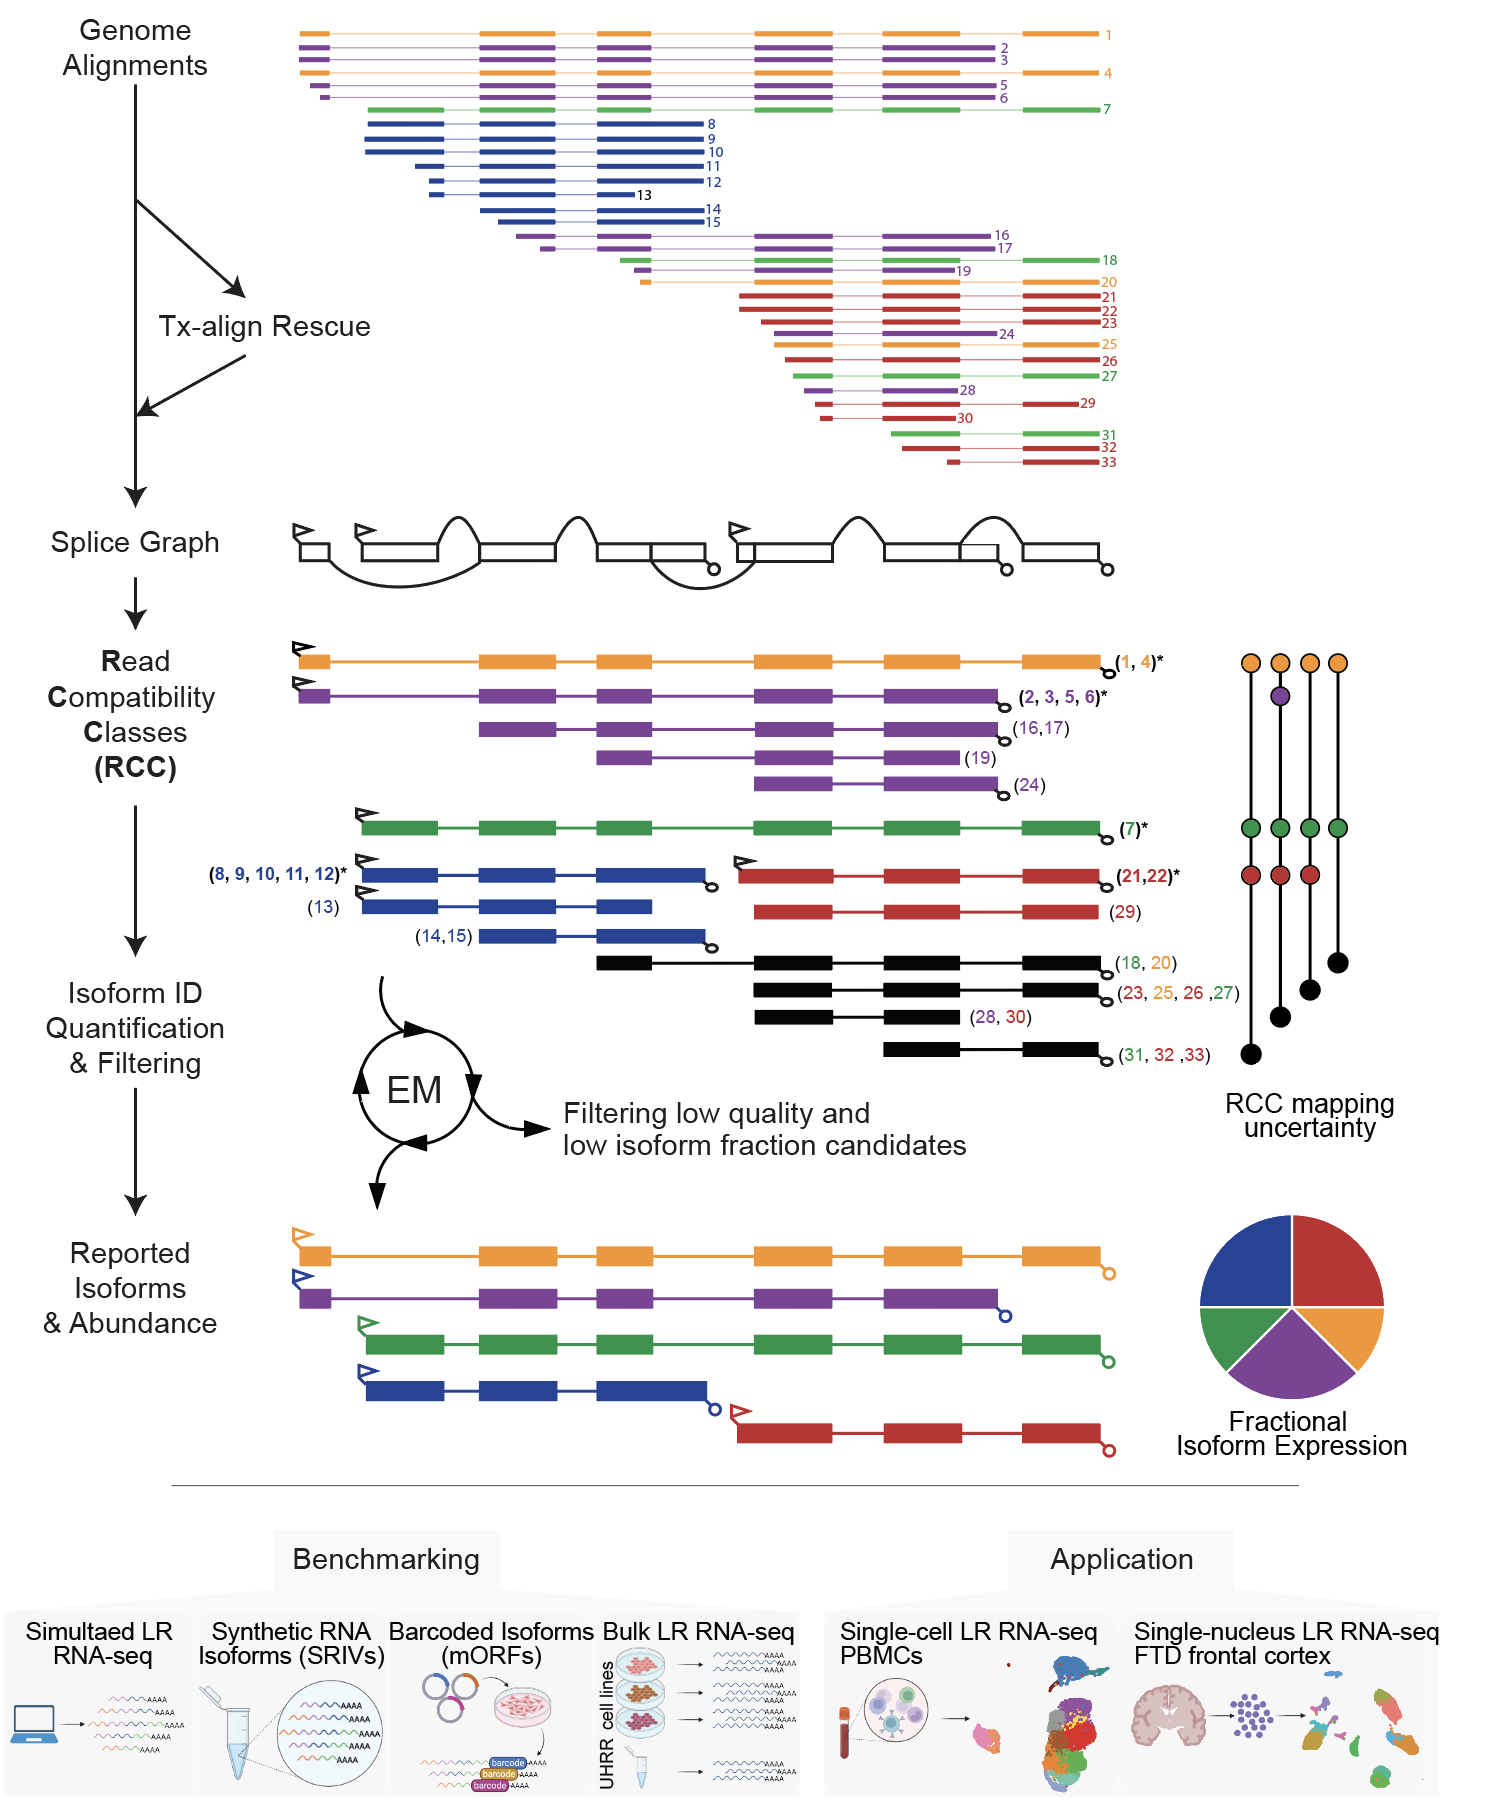
\includegraphics{figures/docx_export/Fig1.png}}
\end{center}

\captionof{figure}{\textbf{Conceptual overview of the LRAA algorithm for isoform identification and quantification in bulk and single-cell long-read transcriptomics.} A simplified overview of the LRAA workflow is shown, beginning with splice-aligned long-read isoform data and encompassing splice-graph construction, assignment of spliced read alignments or rescued direct-to-transcriptome (Tx-align) alignments to genome-based splice graph path nodes and grouping into read compatibility classes (RCC), assembly of candidate isoforms via compatible RCC collapse, and iterative quantification and filtering to define final isoform structures and abundance estimates. For illustrative purposes, read alignments are colored according to the isoforms from which they were derived and numbered to enable visual tracking through the splice graph and RCC relationships; in real RNA-seq data, the transcript of origin for each read is unknown a priori and must be fully inferred from alignment structures and compatibility relationships. Reads are numbered to allow tracking to the splice graph-based RCCs that they define. Top-level RCCs not compatible and contained by other RCCs are labeled with *. \doccomment{Houlin Yu}{2026-07-27}{Here, the sentence says "RCCs found compatible and contained by other top-level RCCs are colored black", my understanding is that here, RCCs are compatible with multiple other top-level RCCs.\\
Maybe I am missing something; If that is the case, I was thinking read 19 may also be black?}\doccomment{Houlin Yu}{2026-07-27}{Also read 29, are we missing a "polyA mark"?}\doccomment{Brian Haas}{2026-07-30}{good catch!~ I added " \textquotesingle splice-incompatible\textquotesingle{} RCCs" to differentiate the black ones.\\
Also, good catch with read 29. That exon should have been shorter than it is. Will update that in the fig.}RCCs found compatible and contained by other top-level splice-incompatible RCCs are colored black and the RCC mapping uncertainty matrix indicates the multiple compatibilities. RCCs with top-level RCC mapping uncertainty have read support fractionally assigned according to the EM. For clarity, several implementation details are abstracted in this schematic; a complete description of the algorithmic workflow is provided in \textbf{Supplementary Figure~\ref{sfig:1}}, which illustrates the construction of separate splice graphs for multi-exon and single-exon read alignments, their subsequent merging, and the downstream quantification and filtering steps. In the schematic, 5′ pointed triangles denote candidate transcription start sites (TSS), and 3′ trailing lollipops denote candidate transcription end sites (TES) or sites of polyadenylation. The LRAA identified isoforms were leveraged for multiple benchmarking and applications as shown (bottom).\doccomment{Houlin Yu}{2026-07-27}{For consistency, RCC mapping uncertainty shall be "RCC Mapping Uncertainty" - the first letter of the word being capitalized}\doccomment{Houlin Yu}{2026-07-27}{Also, "Filtering low qua.." and "FTD frontal.." (not sure about these)}\doccomment{Houlin Yu}{2026-07-27}{mORF, the original cell paper uses all capital letters. MORF}}\label{fig:1}

\subsection{Benchmarking isoform identification and quantification accuracy and study design}\label{benchmarking-isoform-identification-and-quantification-accuracy-and-study-design}

Benchmarking long-read isoform identification and quantification methods is challenging because no single dataset simultaneously provides complete ground truth and the complexity of real biological data. Different benchmarking substrates therefore offer complementary advantages, with each addressing distinct aspects of the problem.

Simulated long-read datasets provide complete knowledge of the isoform from which each read was generated, enabling unambiguous evaluation of isoform identification and abundance estimation even when reads are partial or compatible with multiple isoforms. However, simulated data lack many features of real sequencing experiments, including heterogeneous degradation patterns and the full complexity of transcript processing observed in biological samples, while platform-specific error profiles are necessarily modeled rather than directly observed.

Conversely, genuine long-read RNA sequencing data capture the biological and technical complexity that isoform analysis methods are designed to address, including variable transcript boundaries, partial transcripts, and technology-specific error characteristics. These datasets are therefore essential for evaluating practical performance in biologically relevant settings, but they lack definitive isoform-level ground truth. In particular, it is generally not possible to determine with certainty which isoform a partial read originated from, nor to enumerate all true full-length transcript structures present in a complex sample.

Synthetic spike-in standards, such as SIRVs and Sequins, occupy an intermediate position. These controls consist of real sequence data with defined transcript structures, enabling assessment under controlled conditions. However, because individual reads are not barcoded, the transcript of origin for each read is not directly observable, and these molecules are not expressed within native cellular contexts, limiting their ability to capture biological processing and degradation.

To bridge these gaps, we propose a new benchmarking framework based on Multiplexed Overexpression of Regulatory Factors (MORFs), which provides biologically expressed, barcoded isoforms for which the transcript of origin is known for every sequenced read. MORFs combine key advantages of simulated and real datasets by enabling unambiguous read-level truth assignment while preserving endogenous transcription, degradation patterns, and sequencing error characteristics. This framework allows direct evaluation of isoform discovery, read assignment, and abundance estimation under conditions that closely resemble real experimental data.

Across these benchmarks, definitions of true positives, false positives, and false negatives necessarily depend on both the properties of the dataset and the execution mode being evaluated. For simulated and MORF-based benchmarks, isoform- and read-level truth is explicitly defined, enabling direct assessment of identification and quantification accuracy. In contrast, for genuine whole-transcriptome datasets lacking definitive ground truth, evaluation focuses on structure-based comparisons and quantitative concordance rather than absolute correctness. For reference-guided analyses, isoforms provided as input are excluded from discovery-based performance metrics to ensure that evaluation is restricted to transcripts unknown to the method a priori. Below, we apply all these benchmarking strategies to enable evaluation of isoform identification and quantification performance across the diverse data types and analytical modes.

\subsubsection{Benchmarking isoform identification and quantification accuracy using simulated and genuine PacBio and ONT long isoform reads and reference data sets}\label{benchmarking-isoform-identification-and-quantification-accuracy-using-simulated-and-genuine-pacbio-and-ont-long-isoform-reads-and-reference-data-sets}

To evaluate isoform identification and quantification performance across diverse experimental conditions, we benchmarked LRAA and related methods using PacBio and ONT long-read reference datasets analyzed in the following progression. We first examined simulated long-read datasets, which provide complete knowledge of transcript structures and read origins, enabling direct evaluation of isoform identification and abundance estimation under controlled error models. We next assessed performance using SIRV spike-in controls, consisting of real long-read sequencing data generated from defined transcript mixtures that capture platform-specific error characteristics while retaining known reference structures. Finally, we analyzed MORF datasets, which provide biologically expressed reference transcripts with read-level origin information through isoform barcoding.

\textbf{Simulated long RNA-seq at variable sequencing error}

We evaluated isoform identification and quantification accuracy using simulated long-read strand-specific RNA-seq datasets, which provide a complete and unambiguous ground truth and enable controlled assessment of the impact of sequencing error and read truncation on performance. Long-read data were simulated for mouse and \emph{Arabidopsis thaliana} transcriptomes with platform-specific 3' and 5' end variable truncation at error-free conditions and at increasing total error rates of 1.6\%, 5.0\%, and 8.5\%. Across all simulations and execution modes, LRAA consistently ranked among the top-performing methods for both quantification and isoform identification (\textbf{Figure~\ref{fig:2}, Supplementary Figure~\ref{sfig:2}}). In quantification-only mode, most methods performed well with few exceptions, and LRAA was consistently among the most accurate. For reference-guided and annotation-free isoform identification, LRAA consistently yielded highest overall accuracy (F1 score) across error profiles with the exception of simulated error-free reads where ESPRESSO outperformed all methods in annotation-free isoform discovery. Most methods demonstrated resilience to higher error rates except for ESPRESSO, which continued to perform well but with degraded performance at higher error rates, Mandalorion, and most notably for IsoSeq, which is specifically tuned to PacBio high fidelity (HiFi) reads (\textbf{Supplementary Figure~\ref{sfig:2}}). While informative for contrasting method performance on tractable inputs, simulated data are imperfect models of genuine sequencing data and do not substitute for benchmarking on real datasets.

\paragraph{Spike-In RNA Variants (SIRVs)}\label{spike-in-rna-variants-sirvs}

We next evaluated isoform identification and quantification accuracy using Spike-In RNA Variants (SIRVs), which provide a defined set of transcript structures and relative abundances while retaining real sequencing and alignment characteristics. We analyzed PacBio Kinnex sequencing data for the SIRV mixes E0, E1, and E2, spanning equimolar to highly skewed expression distributions (\url{https://www.lexogen.com/store/sirv-set1/}). Across all three execution modes, LRAA consistently ranked as a top-performing method (\textbf{Figure~\ref{fig:2}, Supplementary Figure~\ref{sfig:3}}), achieving the highest combined precision and recall, as measured by F1 score, in most reference-guided and annotation-free isoform-identification settings. In quantification-only mode, LRAA achieved high accuracy across all SIRV mixes, with other probabilistic approaches including Oarfish, Isosceles, ESPRESSO, and Bambu also performing strongly. For isoform identification, performance varied by execution mode and expression mix. LRAA exhibited top accuracy for ref-guided and de novo isoform identification except for the SIRV E2 mix where ESPRESSO showed marginally higher accuracy in the reference-guided and de novo E2 evaluation. Methods such as IsoSeq and TALON exhibited high sensitivity but lower precision, resulting in reduced overall accuracy. While SIRVs provide a useful intermediate benchmark, they remain synthetic constructs and do not fully reflect native cellular processing of transcripts, which motivated us to explore MORFs as benchmarks described below.

\paragraph{MORFs}\label{morfs}

To benchmark isoform identification and quantification using genuine biological transcripts with unambiguous ground truth, we leveraged the (MORF library \citep{joung2023}. This resource comprises 3,548 human transcription factor isoforms representing 1,836 genes, expressed as lentiviral clones and each containing a unique isoform-specific barcode embedded at the 3′ end of the transcript (\textbf{Supplementary Figure~\ref{sfig:4}a}). These barcodes enable definitive assignment of every sequenced read, including partial reads, to its isoform of origin, thereby overcoming a central limitation of synthetic spike-in controls and genuine transcriptome data. After expressing the MORF library in HEK293 cells, we sequenced it using PacBio Kinnex and ONT MinION. The PacBio dataset represented 2,913 expressed isoforms from 1,560 MORF genes, whereas the ONT dataset represented 2,892 isoforms from 1,553 genes. We used these datasets to evaluate isoform identification and quantification in quantification-only, reference-guided, and annotation-free de novo modes (\textbf{Figure~\ref{fig:2} and Supplementary Figure~\ref{sfig:4}b}). LRAA achieved the highest overall accuracy for both isoform identification and quantification, except for de novo isoform identification mode with ONT where LRAA performed nearly identically to StringTie and ESPRESSO marginally outperformed both. As observed for SIRVs, IsoSeq and TALON exhibited high recall but substantially lower precision, resulting in reduced overall accuracy. Altogether, MORFs provided a more biologically informed benchmark that revealed shifts in relative method performance compared with SIRVs, most notably for Mandalorion, while also confirming that a subset of methods, including LRAA, consistently ranked among the top performers.

\begin{center}
\pandocbounded{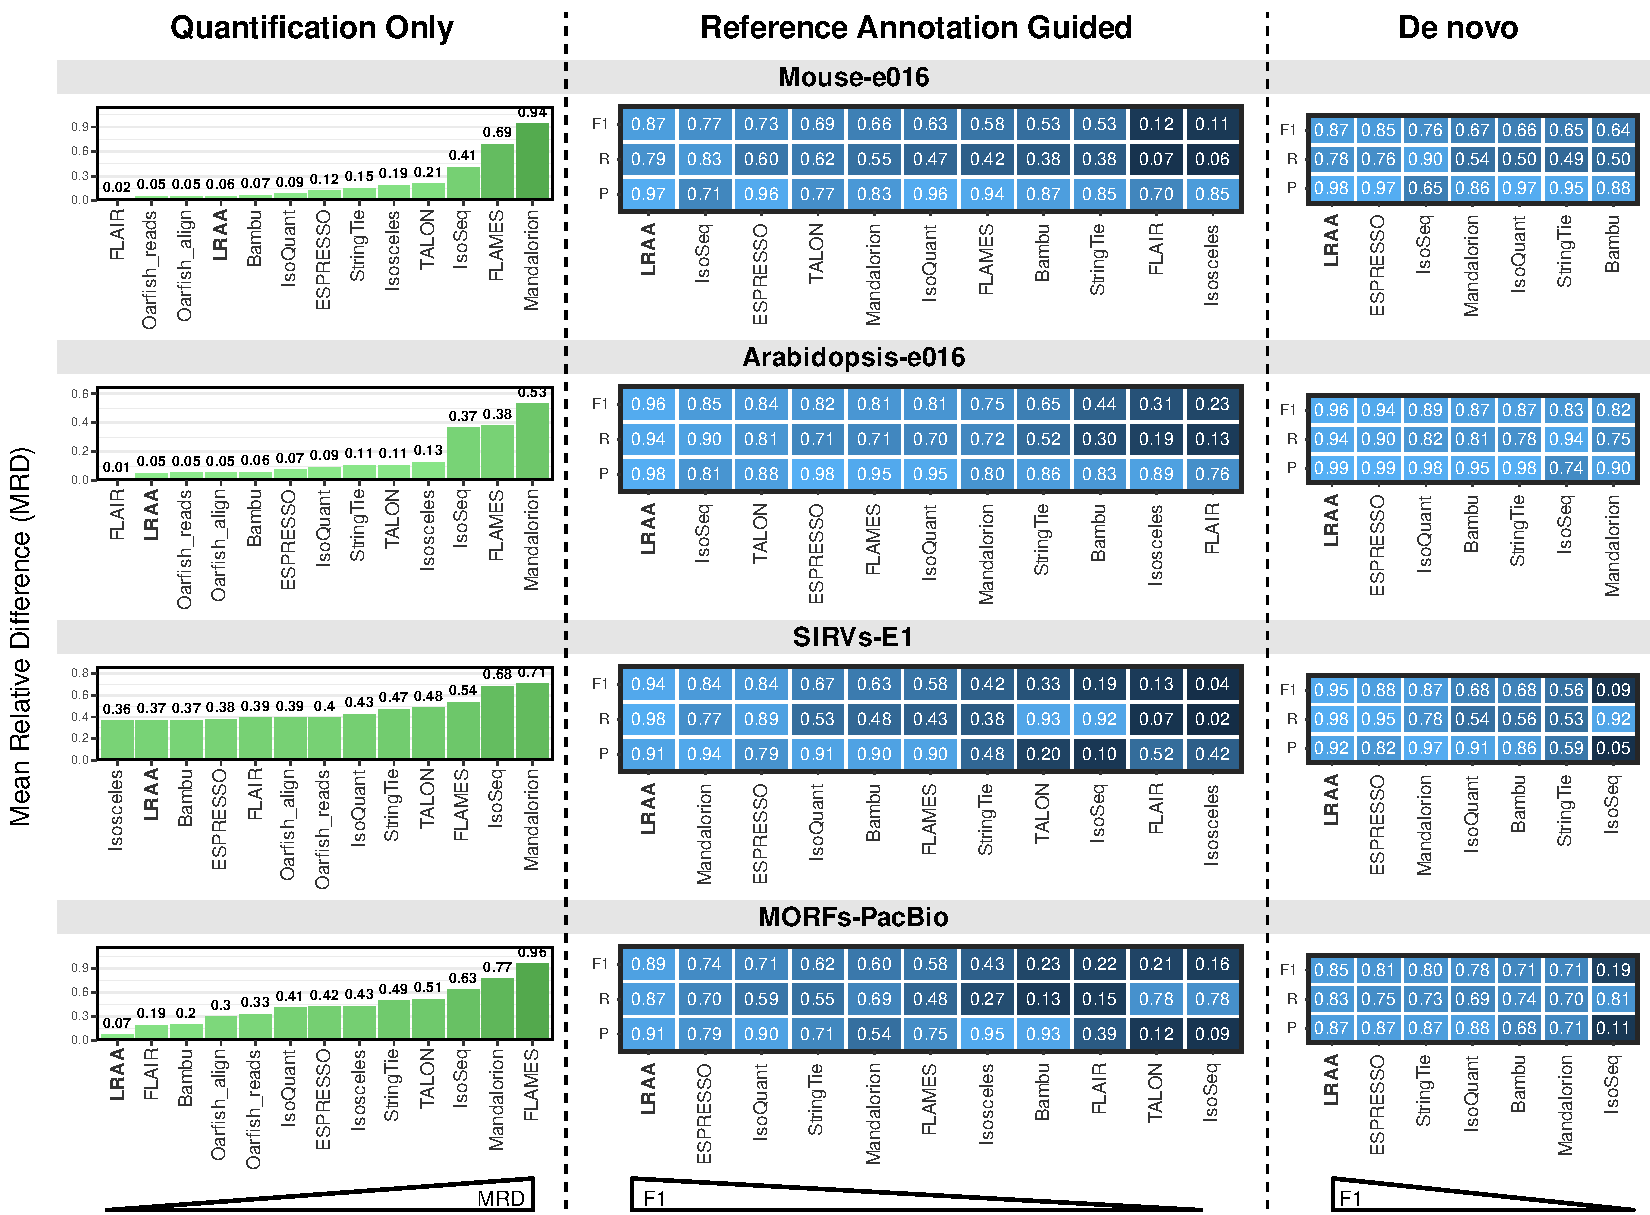
\includegraphics{figures/benchmark/Fig2_benchmarks_sims_SIRVs_MORFs.pdf}}
\end{center}

\captionof{figure}{\textbf{Isoform identification and quantification accuracy based on long read RNA-seq derived from simulated reads (Mouse and Arabidopsis) or genuine RNA-seq for sequencing standards}. Quantification (left column), reference annotation-guided isoform identification (center column), and reference annotation-free (de novo) isoform identification (right column) accuracies are indicated for evaluated methods based on the following data sets (top-to-bottom): simulated mouse and simulated Arabidopsis PacBio reads with 1.6\% error (e016 samples), and genuine PacBio Kinnex sequencing for SIRVs (E1 sample) and MORFs. Methods are ranked from left to right according to top accuracy based on mean relative difference for quantification and F1 score for isoform identification. See \textbf{Supplementary Figures~\ref{sfig:2}-4} for extended sample benchmarks for these targets.}\label{fig:2}

\paragraph{Whole transcriptome sequencing of cell lines and reference standards}\label{whole-transcriptome-sequencing-of-cell-lines-and-reference-standards}

While simulations, SIRVs, and MORFs enable benchmarking against defined truth sets, the primary use case for long-read isoform analysis methods is whole-transcriptome sequencing, where ground truth isoform structures and expression levels are not known. To evaluate performance in this setting, we analyzed bulk long-read transcriptomes generated using PacBio Kinnex for the BT474 and K562 cell lines, the lymphoblastoid sample GM24385 provided as Genome in a Bottle RNA reference sample for individual HG002 (\url{https://www.nist.gov/programs-projects/genome-bottle}), the Universal Human RNA Reference (UHRR) \citep{xu2014}, and Oxford Nanopore strand-specific cDNA sequencing for the A549 and MCF7 cell lines from the SG-NEx project \citep{chen2025}. Isoform identification accuracy was assessed using both reference-guided and annotation-free \emph{de novo} execution modes, with proxy truth sets defined based on agreement across methods and known reference annotations (see \textbf{Methods}). Across all PacBio Kinnex and both ONT datasets, LRAA ranked as the top-performing method for isoform identification in reference-guided execution mode. In de novo mode, ESPRESSO slightly outperformed LRAA on the PacBio Kinnex data sets to be top-ranked (\textbf{Figure~\ref{fig:3}}). In contrast, LRAA demonstrated highest accuracy on both ONT data sets and ESPRESSO was least accurate, suffering from especially low recall while retaining high precision (\textbf{Figure~\ref{fig:3}}).

Because no absolute expression ground truth is available for these datasets, we evaluated quantification consistency by comparing isoform-level expression profiles across methods using Pearson correlation. LRAA-derived expression profiles clustered closely with those from methods that performed best in quantification benchmarks with defined truth sets, including Oarfish, Isosceles, and Bambu. Overall, these results demonstrate that LRAA performs robustly across whole-transcriptome datasets and sequencing platforms, positioning LRAA as a highly effective approach for long-read transcriptome analysis.

\begin{center}
\pandocbounded{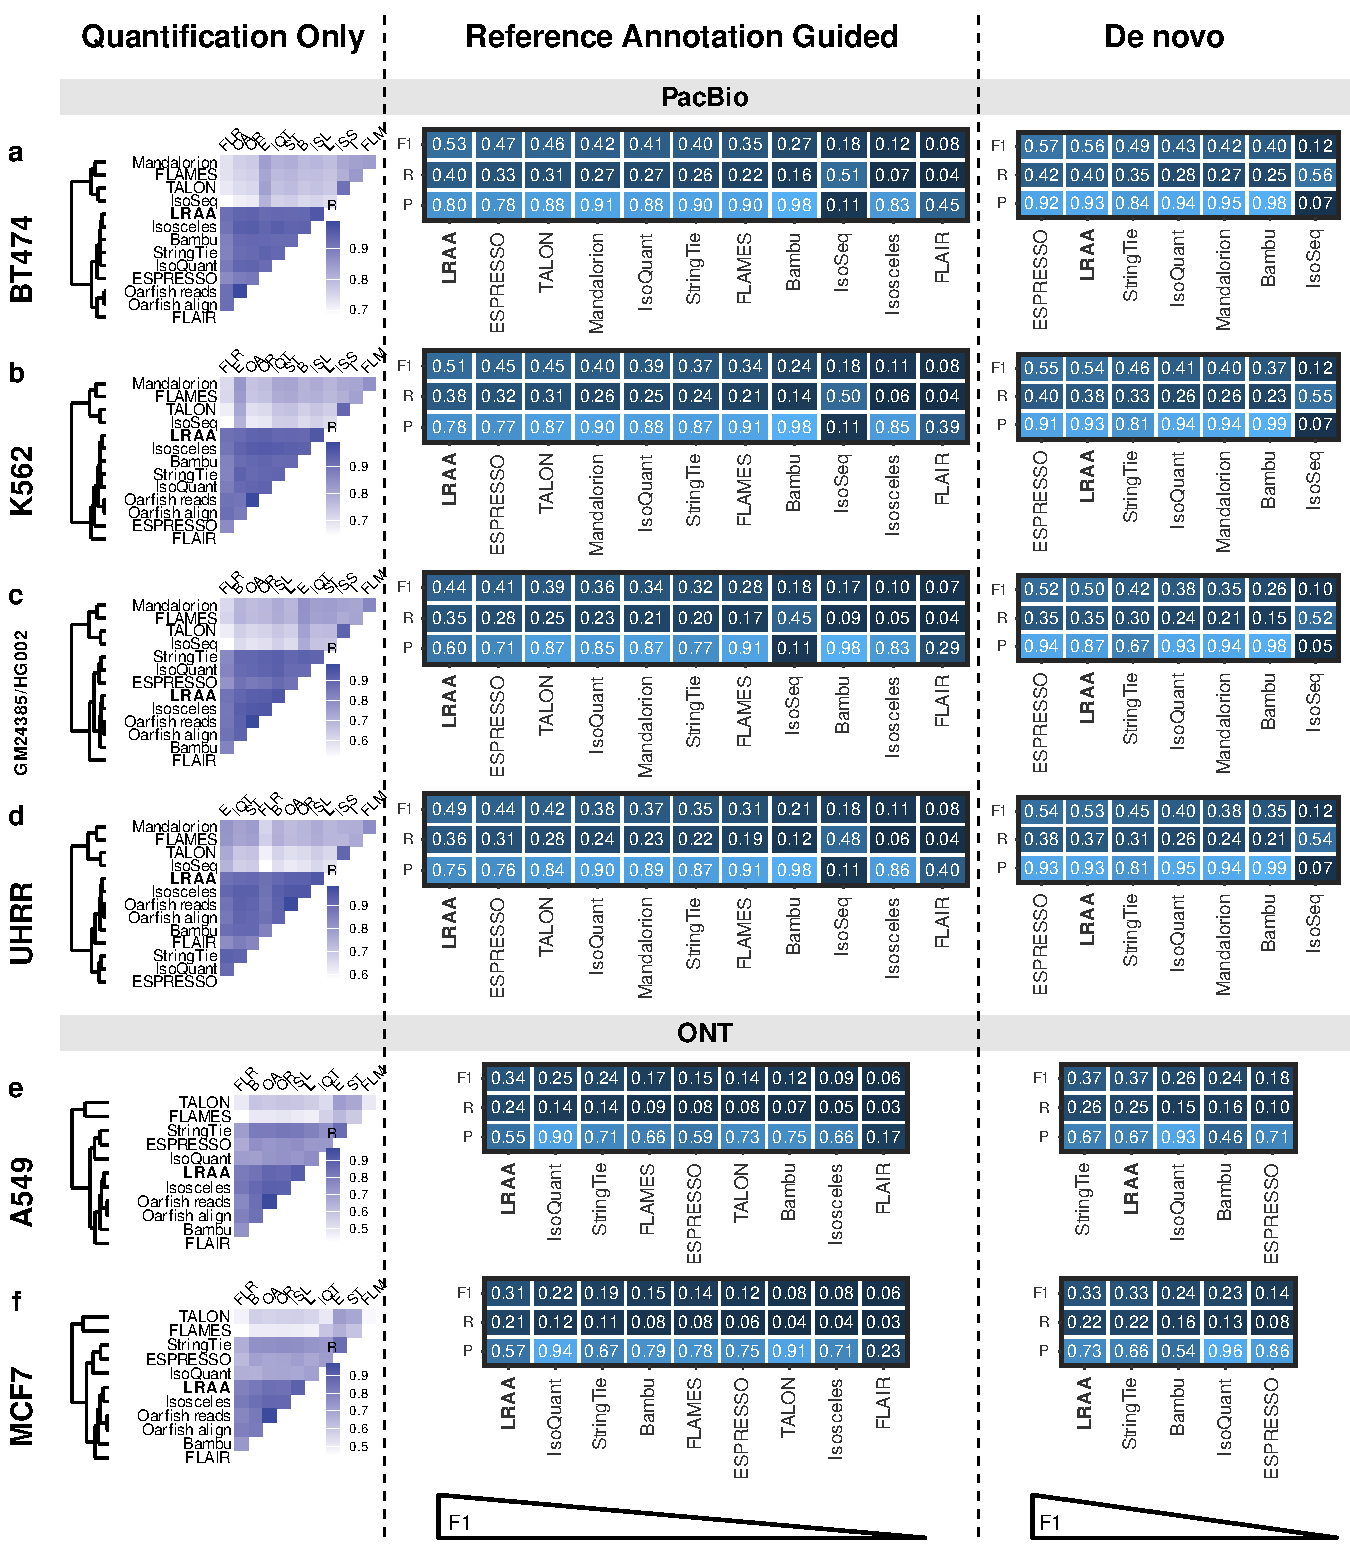
\includegraphics{figures/benchmark/Fig3_benchmarks_cell_lines.pdf}}
\end{center}

\captionof{figure}{\textbf{Benchmarking isoform identification and quantification accuracy using whole transcriptome sequencing of human cell lines and RNA reference samples.} Transcript quantification (left column), reference annotation-guided (center column) and reference annotation-free (de novo) isoform identification (right column) were evaluated for long read isoform analysis methods based on whole transcriptomes sequenced using PacBio Kinnex (top section) or ONT (bottom section). PacBio Kinnex sequenced transcriptomes correspond to (top-to-bottom) cell lines (a) BT474 and (b) K562 and (c) reference standards Genome In a Bottle RNA sample for GM24385/HG002 and (d) commercially available Universal Human RNA Reference (UHRR) from Thermo Fisher Scientific. ONT sequenced cell lines correspond to (top-to-bottom) (e) A549 and (f) MCF7. Expression quantification was evaluated by computing the Pearson correlations for isoform expression (log(TPM+1) values) and clustered by similarity. Isoform identification accuracy was estimated using proxy truth sets based on shared vs. uniquely identified isoforms (see \textbf{Methods}). Abbreviations used: FLR:FLAIR, B:Bambu, OA:Oarfish align, OR:Oarfish reads, L:LRAA, ISL:Isosceles, IQT:IsoQuant, E:ESPRESSO, ST:StringTie, FLM:FLAMES.\doccomment{Houlin Yu}{2026-07-27}{Bottom left MCF7 Quant plot: the labels of tools are a bit misaligned.}}\label{fig:3}

\subsubsection{Application of LRAA for de novo or reference-guided isoform identification in single-cell and single-nucleus long-read whole transcriptome sequencing.}\label{application-of-lraa-for-de-novo-or-reference-guided-isoform-identification-in-single-cell-and-single-nucleus-long-read-whole-transcriptome-sequencing.}

Application of long-read transcriptome sequencing at single-cell and single-nucleus resolution enables isoform-level analysis in heterogeneous tissues but introduces additional computational challenges relative to bulk data \citep{gupta2024, kumari2024, alkhafaji2024, hardwick2022}. In particular, individual cells contribute limited read depth, rare isoforms may be confined to specific cell populations, and single-nucleus data are enriched for partially processed transcripts. To address these challenges, we developed an LRAA single-cell workflow that integrates isoform identification and quantification with cell clustering, allowing isoform discovery to be informed by cell-type-specific expression patterns (\textbf{Figure~\ref{fig:4}}).

The LRAA single-cell workflow operates in two phases. In the first phase, LRAA is applied in pseudobulk mode to perform isoform identification and quantification using either reference-guided or annotation-free execution modes. Gene-level expression estimates derived from this phase can then be used to define cell clusters based on cell-barcoded read assignments or cluster assignments can be predefined by the user. In the second phase, isoform identification is performed separately within each cell cluster guided by the initial pseudobulk-based isoform structures, further enabling recovery of isoforms that are low abundance in the full pseudobulk but enriched within specific cell populations. Isoforms identified across clusters are subsequently merged into a unified isoform set, followed by a final round of cluster-aware quantification to generate gene-, isoform-, and splice-pattern-level expression matrices for downstream analysis.

We applied this workflow to two distinct long-read single-cell datasets generated using PacBio Kinnex sequencing of 10x 3′ libraries: peripheral blood mononuclear cells (PBMCs), representing a well-characterized and transcriptionally diverse cell population, and single nuclei isolated from frontal cortex tissue of an FTD donor, representing a challenging setting dominated by intronic reads and incomplete transcript processing.

\begin{center}
\pandocbounded{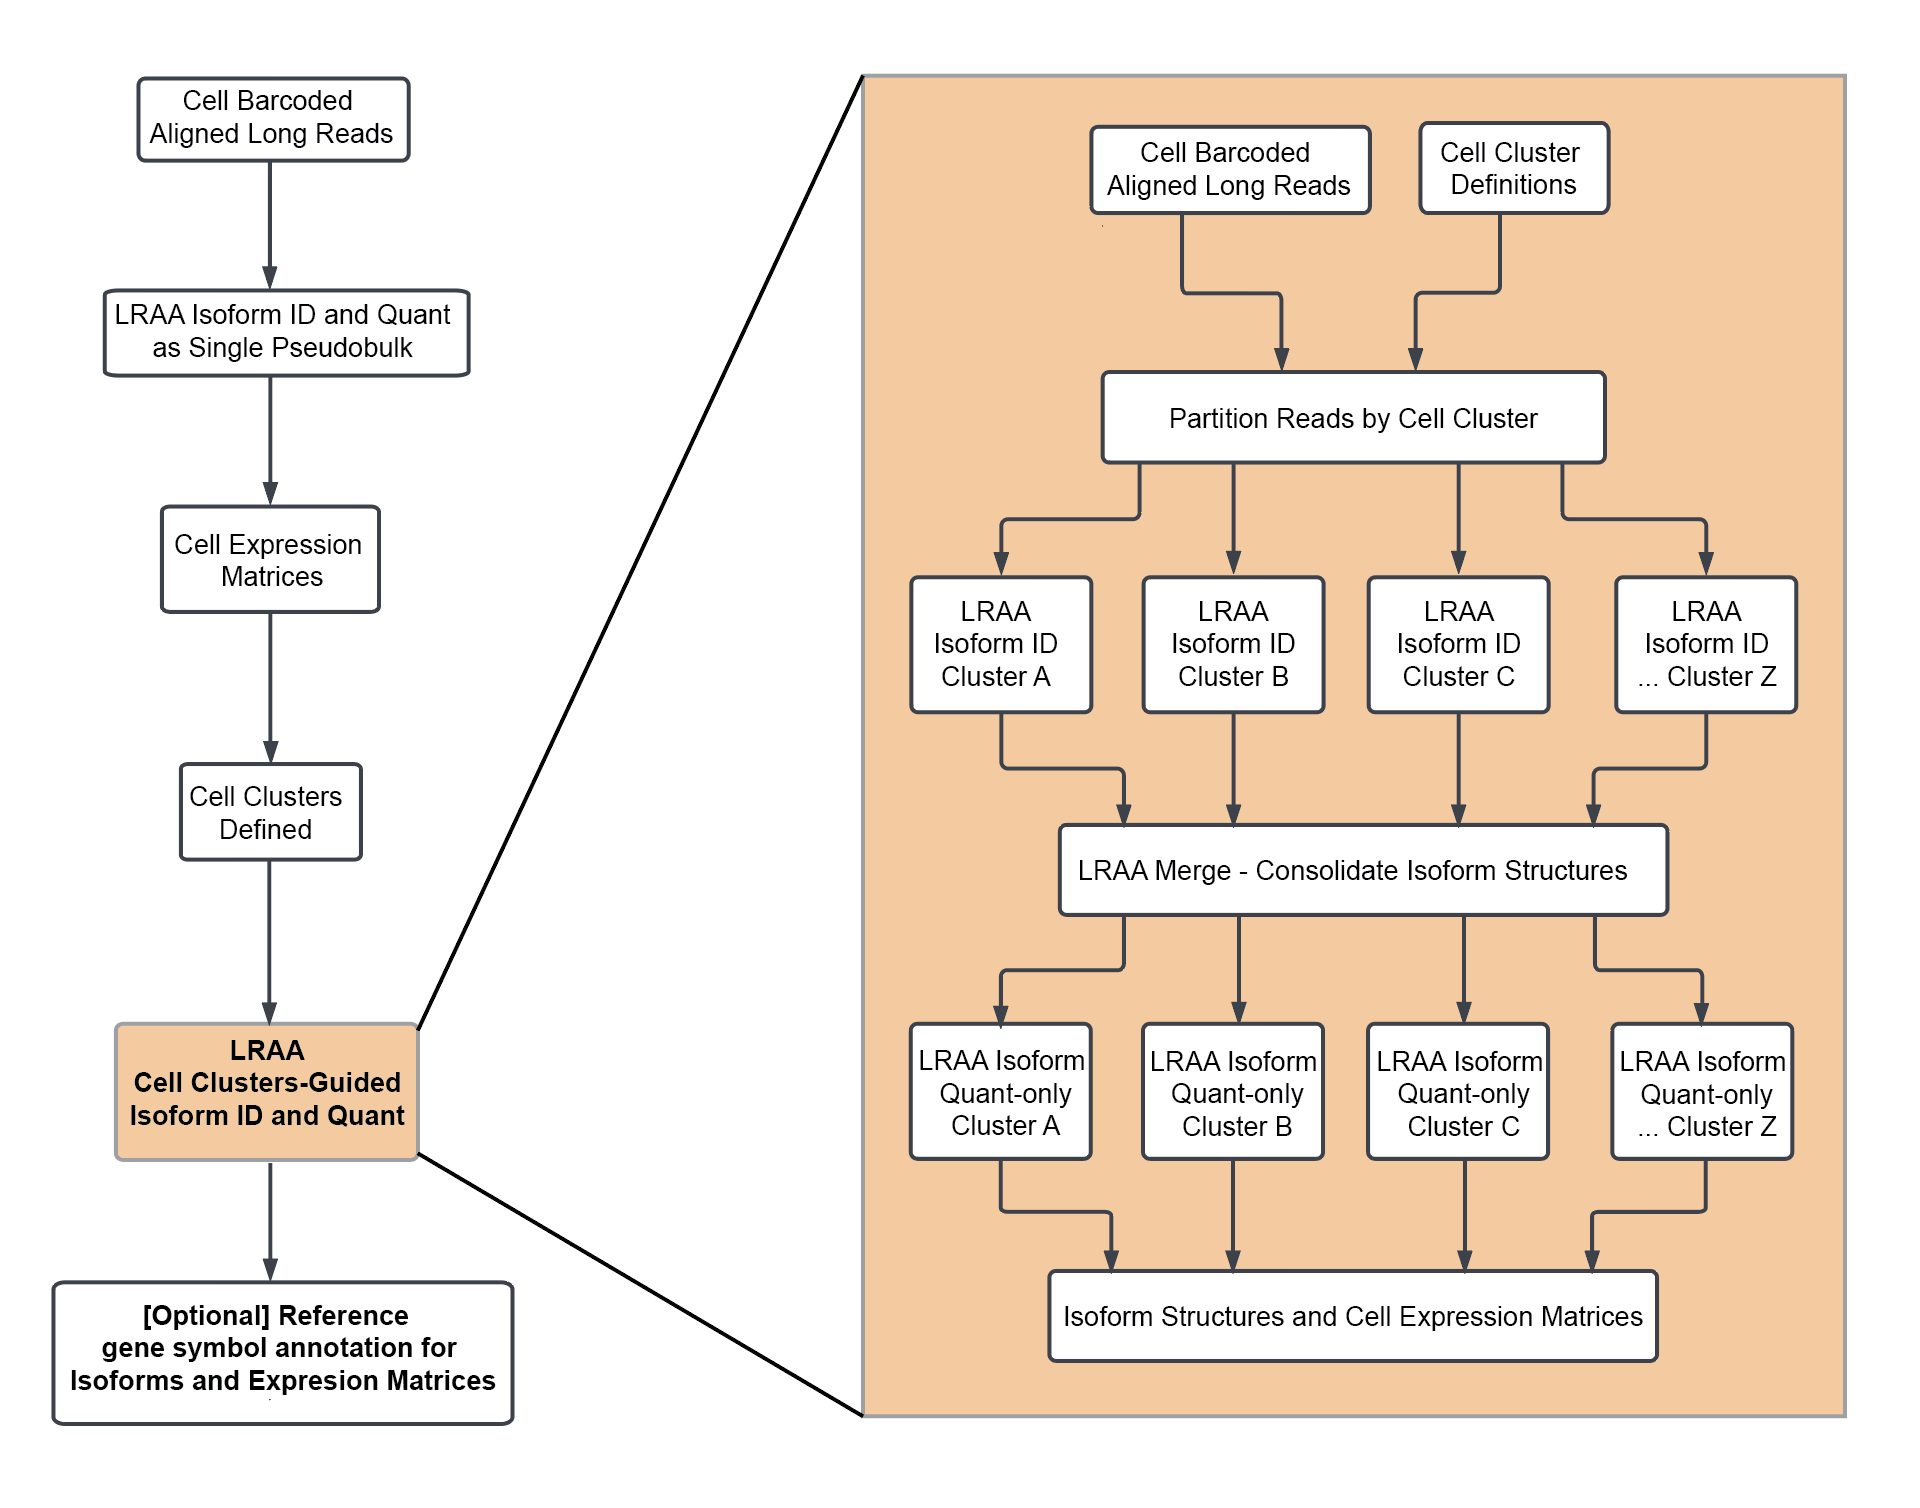
\includegraphics{figures/docx_export/Fig4.png}}
\end{center}

\captionof{figure}{\textbf{Pipeline for application of LRAA to single-cell transcriptomics data for novel isoform discovery.} LRAA is first leveraged for isoform identification and quantification in pseudobulk mode (yellow). Cell barcodes derived from isoform-assigned reads are leveraged to define cell clusters unless predefined as an input. LRAA is then used on a second phase where isoform identification is performed separately on each cell cluster, using the isoform structures defined in the initial phase for reference-guided isoform identification. The cell cluster-based isoforms are subsequently merged and unified followed by a final round of cell cluster-based quantification to assign reads (and cell barcodes) to the unified isoform set, ultimately retaining cell-type specific isoform structures.}\label{fig:4}

\paragraph{Isoform Detection via Single-Cell Kinnex from PBMCs}\label{isoform-detection-via-single-cell-kinnex-from-pbmcs}

We first applied the LRAA single-cell workflow to a PBMC sc-Kinnex dataset generated using PacBio sequencing of a 10x 3′ library totaling 82M reads for 10k cells. We examined the characteristics of individual long-read alignments relative to the reference annotation using an LRAA SQANTI-like classification (see \textbf{Methods}). A substantial fraction of reads corresponded to fully spliced matches (FSM, 29\%) and incompletely spliced matches (ISM, 9\%), with additional reads mapping to intronic or antisense regions (\textbf{Figure~\ref{fig:5}a}).

LRAA was run in both annotation-free de novo and reference-guided modes. To ensure consistent downstream comparisons across pipeline execution modes, instead of using automated within-pipeline cell clustering, we provided predefined cell clusters as a pipeline input and the same cluster assignments were used for subsequent cluster-guided isoform identification and quantification in both execution modes (\textbf{Figure~\ref{fig:5}c}). We compared isoform structures obtained from the initial pseudobulk phase and the final cluster-guided phase of the workflow. The ref-guided and cell cluster-guided phase yielded modest increases in FSM isoforms (9\%) but substantially increased the number of ISM (67\%) and novel isoforms (123\%), while also contributing many more single-exon transcripts, most of which were localized within introns or oriented antisense to annotated transcripts (\textbf{Figure~\ref{fig:5}b}).

Notably, the cluster-guided phase enabled recovery of isoforms that were present at low fractional abundance in the pseudobulk analysis but became prominent within specific cell clusters. Many such isoforms failed to meet minimum isoform fraction thresholds in the initial phase but exceeded these thresholds when evaluated within cluster-specific contexts (\textbf{Figure~\ref{fig:5}d}). Reference-guided execution increased the number of FSM isoforms relative to annotation-free discovery but had limited impact on the recovery of ISM and novel isoforms.

Using the reference-guided, cluster-guided isoform set, we examined differential transcript usage across PBMC cell clusters. We identified genes exhibiting shifts in dominant isoform usage driven by alternative splicing (mean 167 genes per pair of cell clusters), as well as genes with identical splice patterns but alternative transcription start or end site usage (mean 73 genes per pair cell clusters) (\textbf{Figure~\ref{fig:5}e}). Representative examples include isoform switching of \emph{AIF1} between non-classical monocytes and subsets of T cells, and alternative transcription start site usage of \emph{EMP3} across monocytes, dendritic cells, B cells, and T cell populations (\textbf{Figure~\ref{fig:5}f--p}).

To further characterize the functional implications of alternative isoform usage, we examined the protein structural differences between the two proteoforms encoded by alternatively used \emph{AIF1} isoforms across PBMC cell types (\textbf{Figure~\ref{fig:5}k}). Structural modeling revealed that AIF1\^{}6633d encodes a truncated protein containing only a partial EF-hand calcium-binding domain, while AIF1\^{}a9489 encodes the full-length protein with a complete EF-hand domain (\textbf{Figure~\ref{fig:5}k}). Superimposition of the two structures showed extensive overlap, with AIF1\^{}a9489 containing additional structured and unstructured regions that may confer distinct calcium-binding properties and protein-protein interaction capabilities. Both proteoforms matched known reference annotations in GENCODE v47, demonstrating that reference-annotated alternative splicing can generate proteoforms with substantially different structural and potentially functional properties.

These findings motivated us to systematically investigate the landscape of novel proteoforms, those arising from unannotated splice junctions or intron retention events, that may expand proteomic diversity beyond the reference annotation. To identify novel proteoforms in human PBMCs, we applied our classification pipeline to complete ORF protein sequences at three length thresholds (≥50 AA, ≥100 AA, ≥200 AA). At the ≥50 AA threshold, 80,661 unique proteins were detected, with novel proteoforms representing 13.4\% (10,844) of the total proteome (\textbf{Supplementary Figure~\ref{sfig:6}, top}). Notably, as stringency increased to ≥100 AA and ≥200 AA, the proportion of novel proteoforms remained more or less consistent at 14.0\% (8,365 of 59,923) and 12.6\% (4,572 of 36,325), respectively, indicating that novel splicing events generate proteoforms across the full spectrum of protein sizes. Analysis of novel proteoform composition revealed that novel splice junctions accounted for 81.8-85.2\% of novel proteoforms across all thresholds, while intron retention events contributed 14.2-17.6\%. A combination of both mechanisms accounted for 0.6-0.7\% of novel proteoforms. (\textbf{Supplementary Figure~\ref{sfig:6}, bottom}).

\begin{center}
\pandocbounded{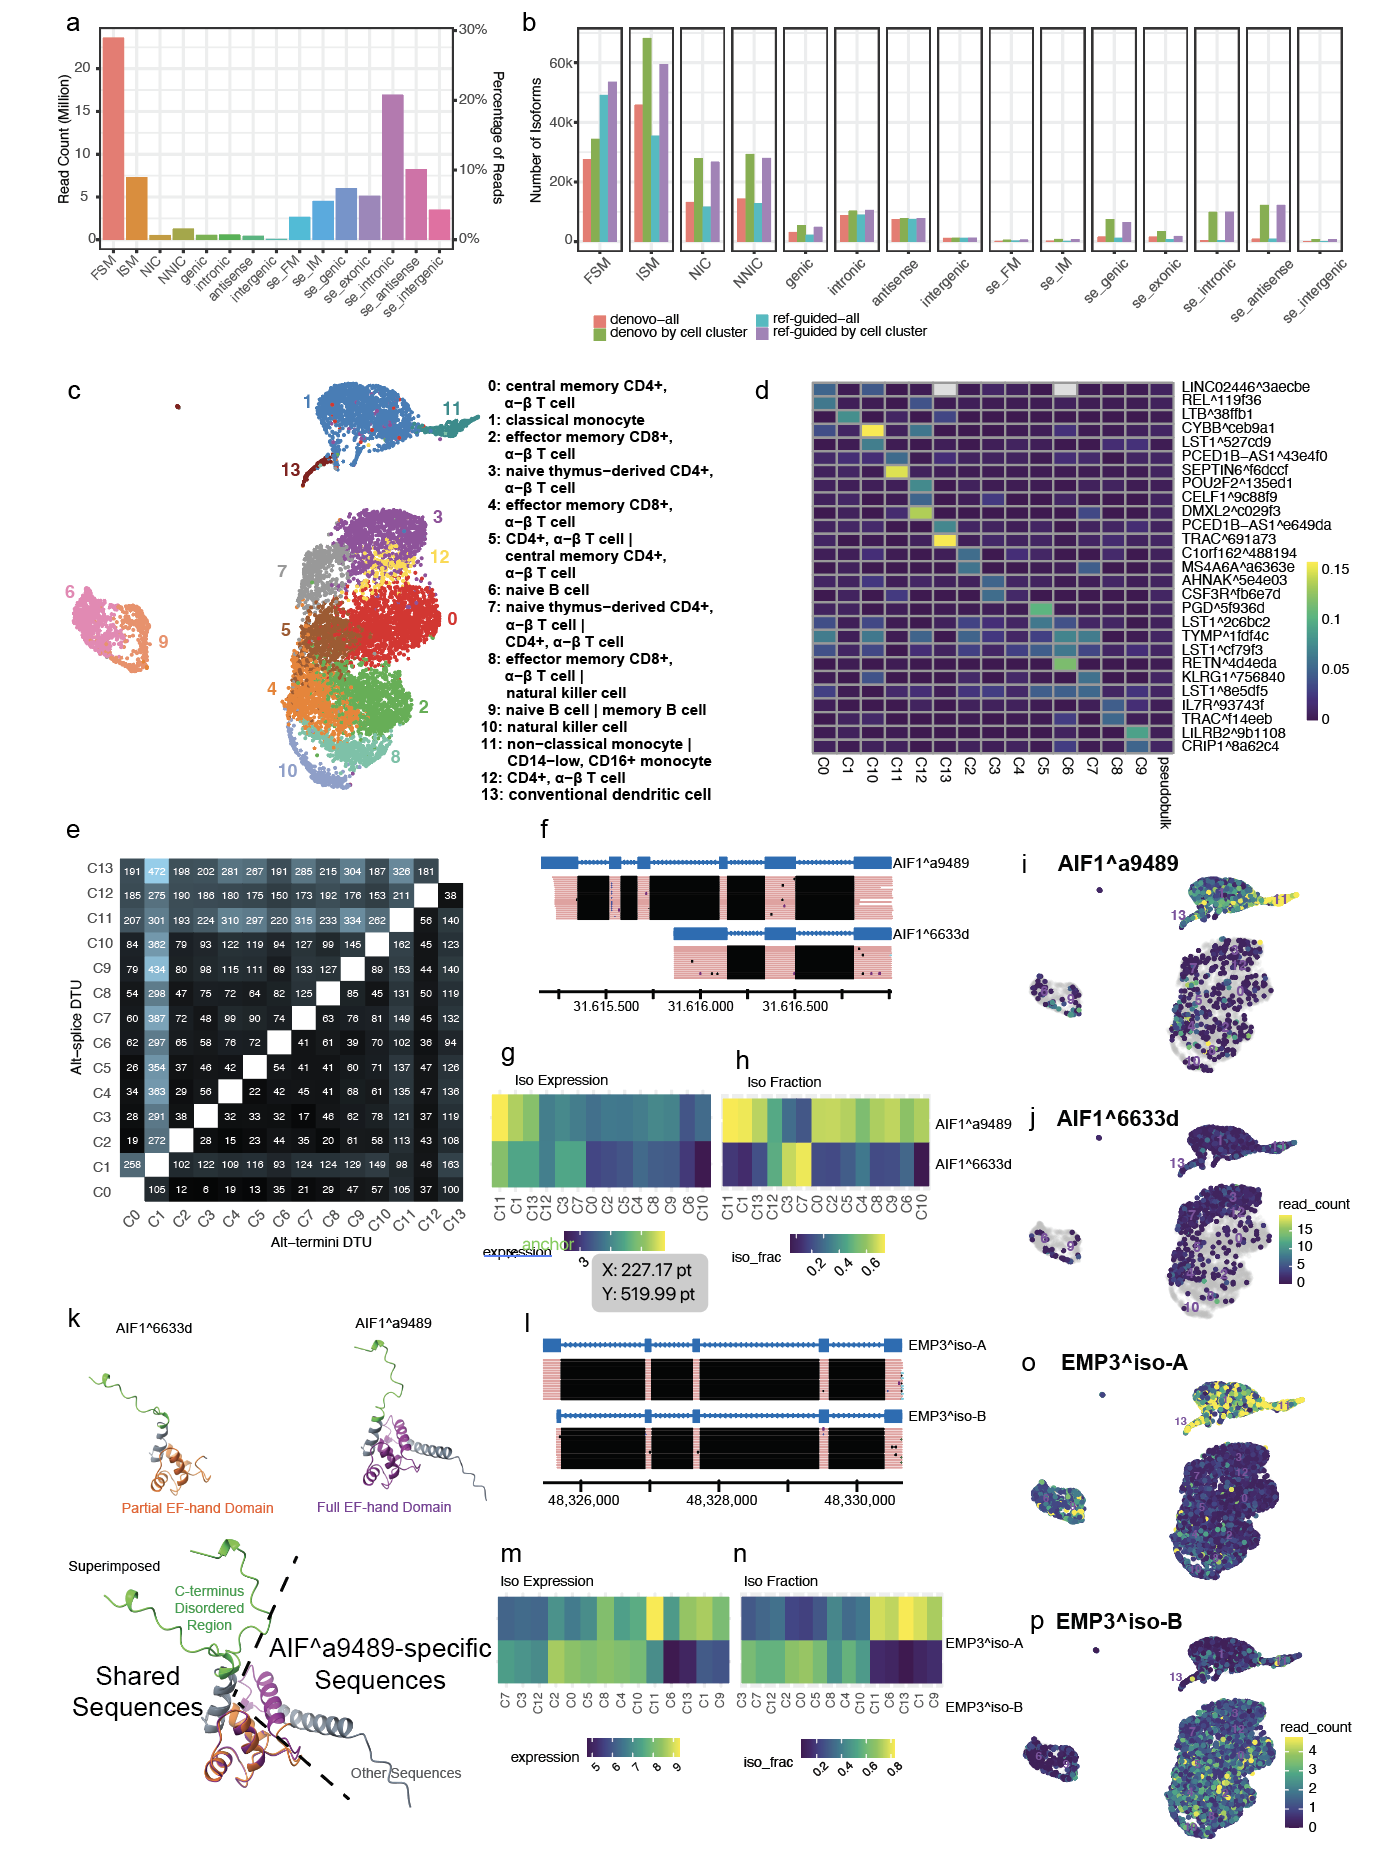
\includegraphics{figures/docx_export/Fig5.png}}
\end{center}

\captionof{figure}{\textbf{Isoform identification and quantification in PBMCs via LRAA with Kinnex scRNA-Seq.} (a) Counts and percentages of Kinnex reads assigned to gene structures or genome regions according to LRAA SQANTI-like categories. (b) Counts of LRAA-reconstructed isoforms from reference annotation-free (de novo) or reference annotation-guided workflows assigned to SQANTI-like categories. Isoforms with identical splice patterns but different termini boundaries are counted non-redundantly as collapsed. (c) UMAP for PBMCs based on LRAA-derived gene expression in quantification-only mode with dominant inferred cell types indicated. (d) Examples of isoforms estimated to have \textless1\% isoform fraction in pseudobulk mode but ≥ 5\% isoform fraction in at least one cell cluster context. (e) Counts of genes with detected differential transcript usage (DTU, upper triangle) or having identical splicing patterns but alternative termini usage (ATU, lower triangle) by cell cluster comparison. (f-j) DTU detected for two isoforms of the AIF1 gene with (f) isoform structures and supporting full-length Kinnex reads, (g) isoform expression, (h) isoform fraction, and (i,j) cellular expression shown for each isoform. (k) Structural modeling of AIF1 proteoforms. (l-p) ATU in the form of alternative transcriptional start sites detected for two isoforms of the EMP3 gene with (l) isoform structures and supporting full-length Kinnex reads, (m) isoform expression, (n) isoform fraction, and (o,p) cellular expression shown for each isoform.\doccomment{Houlin Yu}{2026-07-27}{5g, bottom, we have some unwanted elements}\doccomment{Houlin Yu}{2026-07-27}{m and n, right side, the isofrom ids are misaligned}}\label{fig:5}

\paragraph{Isoform Detection in Single-Cell Nuclei from an FTD Brain Frontal Cortex Sample}\label{isoform-detection-in-single-cell-nuclei-from-an-ftd-brain-frontal-cortex-sample}

We next applied the LRAA single-cell workflow to long-read single-nucleus RNA-seq data generated from frontal cortex tissue of an FTD donor. Single-nucleus sequencing enables transcriptional profiling of cell types that are difficult to capture using whole-cell approaches, but the resulting data are enriched for unspliced and partially processed transcripts, posing challenges for isoform-level analysis.

The FTD frontal cortex dataset was generated using PacBio Kinnex sequencing of a 10x 3′ single-nucleus library, yielding approximately 55 million long reads for 6.5k nuclei. In contrast to the PBMC sc-Kinnex data, the largest fraction of reads was classified as intronic (42\%), combining both intronic categories in the LRAA SQANTI-like read classification, with substantially fewer reads corresponding to fully spliced matches (3\%) or incompletely spliced matches (4\%) (\textbf{Figure~\ref{fig:6}a}). Despite this, LRAA identified large numbers of isoforms in both annotation-free and reference-guided execution modes; in the initial pseudobulk phase, reference-guided analysis yielded approximately three times as many fully spliced isoforms as annotation-free analysis (\textbf{Figure~\ref{fig:6}b}). For cluster-guided isoform identification, we similarly provided predefined cell clusters as input to the pipeline to enable consistent comparisons across clusters.

Comparison of the initial pseudobulk phase and the cluster-guided phase showed limited differences in the number of fully spliced matched isoforms, but substantial increases in incompletely spliced matched (25\% increase for de novo and 55\% increase for reference-guided) and novel isoforms (37\% increase for de novo and 56\% increase for reference-guided) following cluster-guided isoform discovery (\textbf{Figure~\ref{fig:6}b}). The abundance of intronic reads did not lead to a proportional increase in intronic isoform calls, consistent with LRAA\textquotesingle s stringent filtering based on read support, transcription start site evidence, and transcript end site evidence.

Gene-level expression profiles derived from the quantification-only phase were used to identify 14 distinct cell clusters corresponding to major brain cell types, including excitatory and inhibitory neurons, astrocytes, oligodendrocytes, microglia, endothelial cells, and fibroblasts (\textbf{Figure~\ref{fig:6}c,d}). Several of these cell types were further resolved into transcriptionally distinct subpopulations, often differing substantially in the number of expressed genes per nucleus (\textbf{Figure~\ref{fig:6}d}). Pairwise differential expression analysis between paired cell type subpopulations coupled with functional enrichment analysis indicated one subpopulation to be generally more active than the other coupled with stress responses. We refer to these as active or quiescent subpopulations below.

Using the reference-guided, cluster-guided isoform set, we examined differential transcript usage across cell clusters. Despite the predominance of intronic reads, we identified genes exhibiting significant shifts in isoform usage between cell types (\textbf{Figure~\ref{fig:6}e}). Among these, we detected the pathogenic cryptically spliced isoform of \emph{STMN2}, a hallmark of TDP-43 proteinopathy in FTD (\textbf{Figure~\ref{fig:6}f--j}) \citep{prudencio2020, melamed2019, klim2019}. Expression of \emph{STMN2} transcripts was most prevalent in excitatory neuron clusters 8 and 1, where \emph{STMN2} expression was detected in 40\% and 37\% of nuclei, respectively. However, the fraction of nuclei expressing the cryptically spliced isoform differed substantially between these clusters, with 18\% of active cluster 8 nuclei showing evidence of the cryptic isoform compared to 9\% in quiescent cluster 1. Inhibitory neuron clusters (active) 4 and (quiescent) 6 also exhibited \emph{STMN2} expression in 18\% and 10\% of nuclei, respectively, but the cryptically spliced isoform was detected in only 2\% and 1\% of nuclei in these clusters.

In addition to alternative splice pattern usage, we identified cases of alternative transcript end site usage without changes in splice structure. One such example involved \emph{EIF1}, where isoforms with identical splicing patterns but distinct polyadenylation sites were detected across multiple cell types, with the most pronounced shifts observed between oligodendrocytes and endothelial cells (\textbf{Figure~\ref{fig:6}k--o}).

We applied the same proteoform analysis pipeline to FTD brain frontal cortex samples. Novel proteoforms represented 5.5\% (3,639 of 66,109), 5.9\% (2,775 of 46,967), and 5.0\% (1,403 of 27,998) of the total proteome at ≥50 AA, ≥100 AA, and ≥200 AA thresholds, respectively (\textbf{Supplementary Figure~\ref{sfig:7}}). Consistent with PBMC samples, novel junctions predominated across all thresholds (65.6-72.9\%), while intron retention contributed 26.5-33.9\%. A combination of both mechanisms accounted for 0.5-0.6\% of novel proteoforms.

\begin{center}
\pandocbounded{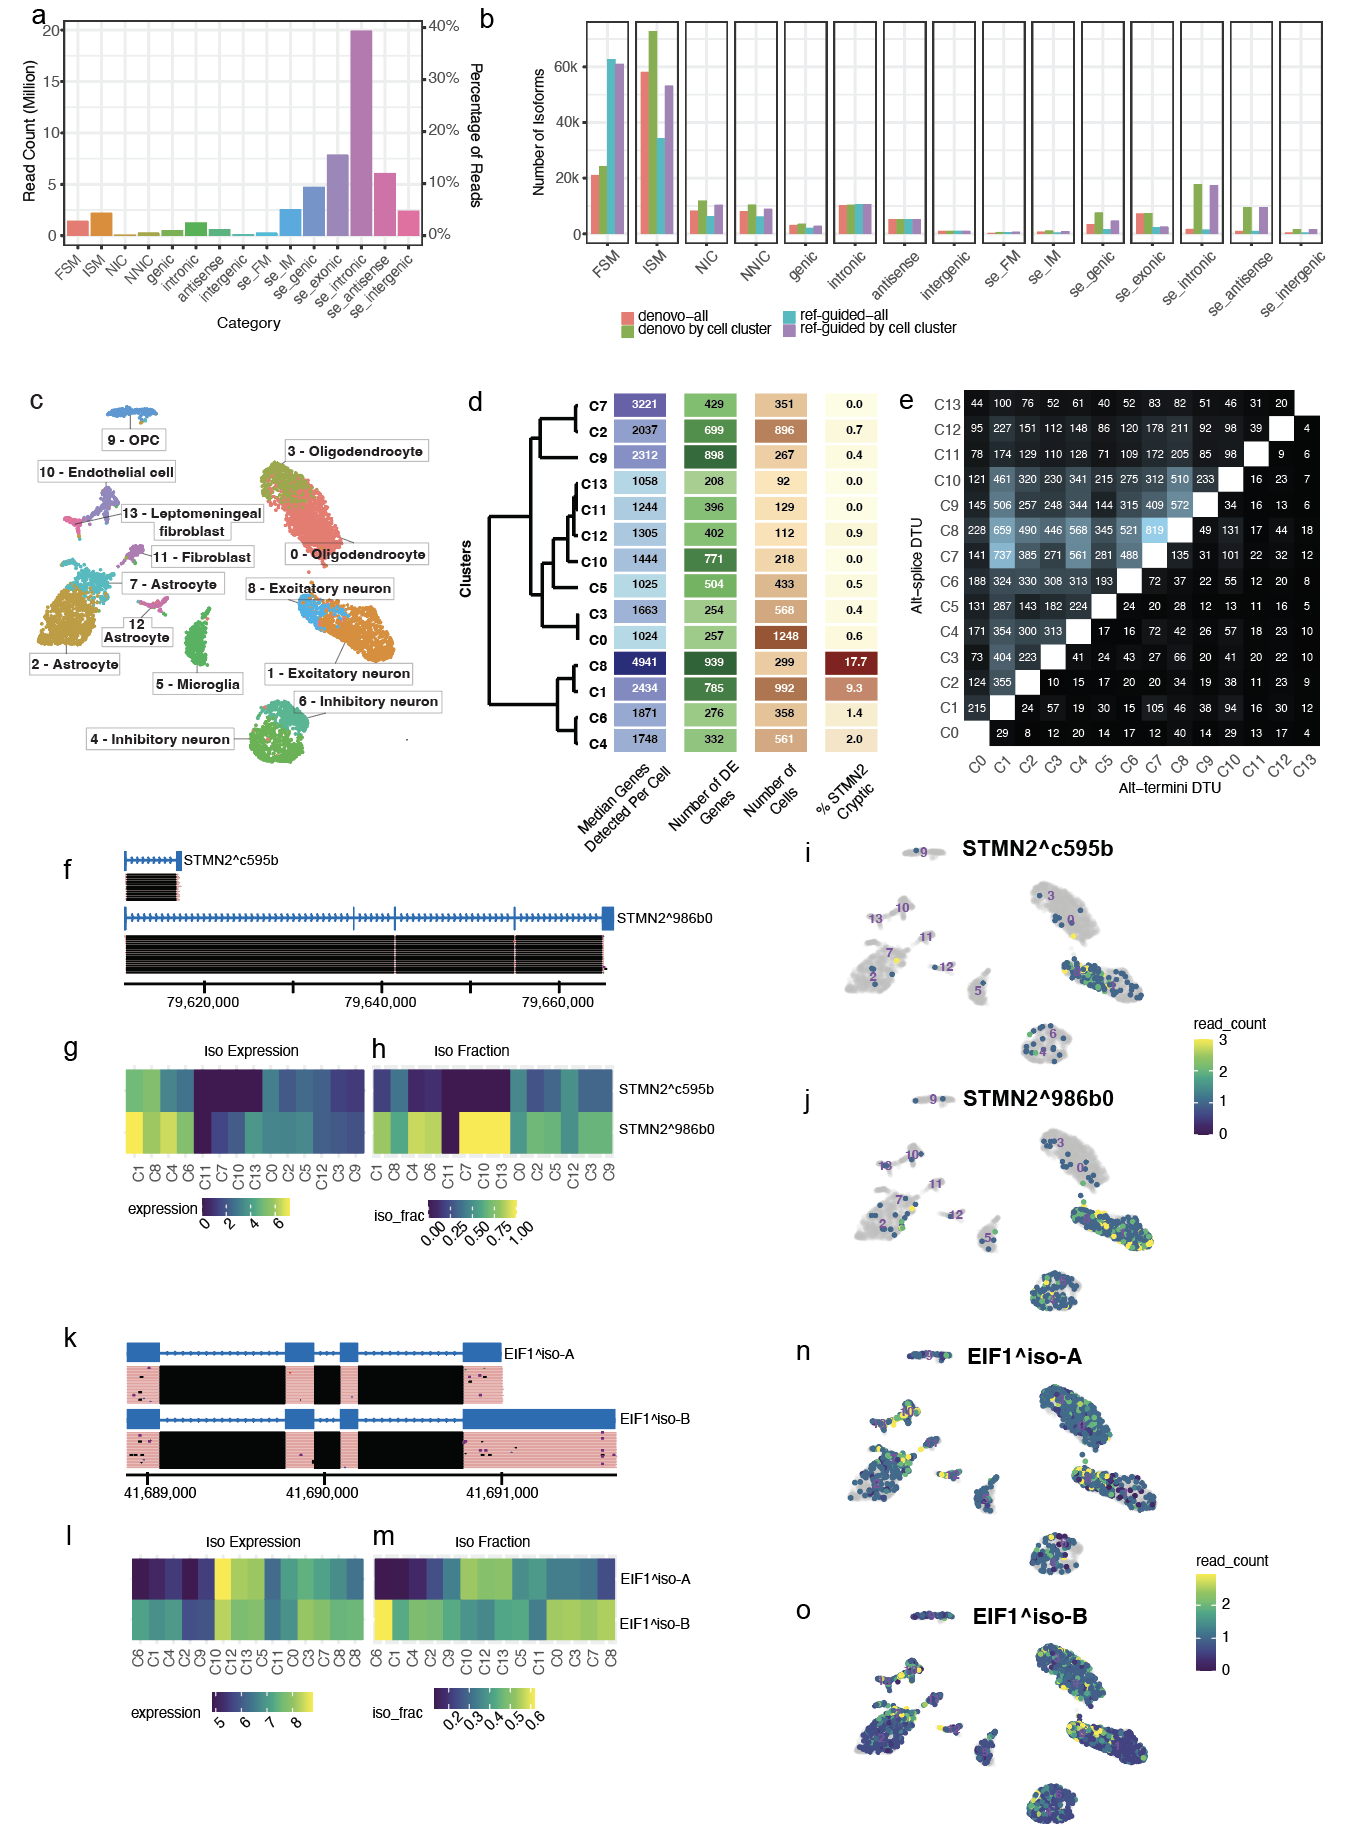
\includegraphics{figures/docx_export/Fig6.png}}
\end{center}

\captionof{figure}{Isoform identification and quantification in an FTD brain frontal cortex via LRAA with Kinnex snRNA-Seq. (a) Counts and percentages of Kinnex reads assigned to gene structures or genome regions according to LRAA SQANTI-like categories. (b) Counts of LRAA-reconstructed isoforms from reference annotation-free (de novo) or reference annotation-guided workflows assigned to SQANTI-like categories. (c) UMAP for FTD frontal cortex sample based on LRAA-derived gene expression in quantification-only mode with dominant inferred cell types indicated. (d) Overview of cell cluster properties and dendrogram showing relationships between cell clusters based on numbers of differentially expressed genes defined as cluster-specific biomarkers \doccomment{Houlin Yu}{2026-07-27}{Do we need these~details here?}\doccomment{Houlin Yu}{2026-07-30}{@bhaas@broadinstitute.org~ will double-check style and whether we need}(p\_val\_adj \textless{} 1e-5 \& abs(avg\_log2FC) \textgreater= 2). (e) Counts of genes with detected differential transcript usage (DTU, upper triangle) or having identical splicing patterns but alternative termini usage (ATU, lower triangle) by cell nuclei cluster comparison. (f-j) DTU detected for two isoforms of the \emph{STMN2} gene with (f) isoform structures and supporting full-length Kinnex reads, with the pathogenic cryptic isoform at top and canonical \emph{STMN2} isoform at bottom, (g) isoform expression, (h) isoform fraction, and (i,j) cellular expression shown for each isoform. (k-o) ATU in the form of alternative polyadenylation sites detected for two isoforms of the \emph{EIF1} gene with (k) isoform structures and full-length Kinnex reads, (l) isoform expression, (m) isoform fraction, and (n,o) cellular nuclei expression shown for each isoform.}\label{fig:6}

\section{Discussion}\label{discussion}

Long-read transcriptome sequencing has transformed transcriptome analysis by enabling direct observation of full-length isoforms rather than inference from short-read fragments. Recent gains in throughput and accuracy have extended these capabilities to single-cell and single-nucleus settings, creating new opportunities to study isoform regulation in heterogeneous tissues and disease. At the same time, these advances have exposed persistent computational challenges, including partial transcript coverage, ambiguous read-to-isoform compatibility, and dependence on incomplete reference annotations. Addressing these challenges requires methods that integrate accurate isoform discovery with principled quantification and that generalize across sequencing platforms and experimental contexts.

Here we present LRAA as a unified framework for isoform identification and quantification from long-read RNA sequencing data spanning bulk, single-cell, and single-nucleus applications. LRAA integrates splice-graph--based structural modeling with an expectation--maximization framework for abundance estimation, enabling probabilistic resolution of ambiguous reads while retaining sensitivity to novel isoforms. Across a broad range of benchmarking datasets, LRAA demonstrated robust performance across execution modes, sequencing technologies, and biological settings. In evaluations that included leading methods assessed by the LRGASP Consortium, such as IsoQuant, Bambu and StringTie, LRAA ranked among the strongest-performing approaches in quantification-only, reference-guided, and de novo analyses. In cases where LRAA did not achieve the highest overall accuracy, its performance closely matched that of the top-ranked method.

Rigorous benchmarking of long-read isoform analysis methods remains challenging because no single dataset simultaneously provides complete ground truth and biological realism. Simulated datasets offer unambiguous isoform-of-origin information and are valuable for controlled evaluation of algorithmic behavior, including sensitivity to sequencing error. However, simulations necessarily lack native transcriptional processing and degradation. Synthetic spike-in controls such as SIRVs incorporate real sequencing characteristics and defined expression ratios, but remain artificial constructs that do not fully reflect cellular transcript processing. As a result, method performance on simulations or spike-ins does not always generalize to biologically complex datasets.

To address this gap, we leveraged the MORF library as a biologically informed benchmarking substrate. MORFs consist of thousands of human isoforms expressed in living cells, each tagged with an isoform-specific barcode that enables unambiguous assignment of every read, including partial reads, to its isoform of origin. This design combines the ground-truth clarity of simulations with the biological context of native transcription. MORF benchmarking revealed certain tools to have notable differences in relative method performance compared with benchmarks on SIRVs, while others, such as LRAA, maintained consistently strong performance across benchmarking conditions. These results underscore the value of biologically inspired benchmarks for realistic evaluation of long-read isoform analysis tools.

Beyond controlled benchmarks, we evaluated LRAA on whole-transcriptome datasets from multiple human cell lines and reference RNA samples sequenced using both PacBio and ONT technologies. In this setting, where absolute ground truth is unavailable, LRAA showed strong performance for isoform identification and produced expression profiles that closely matched those of methods previously shown to perform well under benchmarks with defined truth sets. These results indicate that LRAA generalizes effectively to real-world transcriptome analyses and performs robustly across sequencing platforms without requiring platform-specific workflows.

A major advance of this work is the extension of isoform-resolved long-read analysis to single-cell and single-nucleus transcriptomics. Single-cell long-read data are sparse, and biologically relevant isoforms may be confined to specific cell populations and obscured in pseudobulk analyses. By integrating isoform discovery with cell clustering, LRAA enables recovery of isoforms that are low abundance at the sample level but prominent within particular cell types. In PBMCs, this approach revealed cell-type-specific isoform usage driven by both alternative splicing and alternative transcript start or end site selection.

Single-nucleus transcriptomics presents additional challenges, as nuclear RNA is enriched for unspliced and partially processed transcripts. Despite these constraints, LRAA identified biologically meaningful isoform usage in single-nucleus data from FTD frontal cortex tissue. In particular, we detected the pathogenic cryptically spliced isoform of \emph{STMN2}, a hallmark of TDP-43 proteinopathy, with marked differences in prevalence across neuronal subpopulations. These observations demonstrate that long-read single-nucleus sequencing, coupled with appropriate computational modeling, can resolve disease-relevant isoform dysregulation in tissues that are poorly represented in conventional single-cell approaches. \tofix{Transcript termini need more care in nuclei. Reads from the FTD nuclei, and neuronal nuclei in particular, rarely reached the 5\textquotesingle{} end of their transcripts, and the apparent TSS switches between neurons and other cells were dominated by downstream sites without CAGE support, whereas PolyA sites were as reliable as in PBMCs. Template-switching library preparation leaves an extra, untemplated G at the 5\textquotesingle{} end of molecules copied from capped RNA \citep{wulf2019, cumbie2015}, and in the Kinnex single-cell data this signature separated reads starting at a TSS from truncated reads and marked the FTD downstream sites as truncation. The signature is not specific to Kinnex single-cell libraries: in the bulk PacBio and ONT cDNA libraries benchmarked here, 74\% and 28--29\% of reads starting at annotated TSSs carried one G more than the library's baseline, against 6--7\% and 3\% of reads starting inside transcript bodies, whereas the 5\textquotesingle{} ends of the uncapped SIRV spike-ins in the same PacBio libraries carried it no more often than their transcript bodies (3\%). The baseline itself differed between protocols (no G for single-cell Kinnex, one for bulk PacBio, and three for ONT reads retaining the strand-switching primer), and it is lost where 5\textquotesingle{} clips are trimmed before alignment. A future version of LRAA could use this signature, calibrated per library against reads starting inside transcript bodies, when calling TSS sites and pruning 5\textquotesingle{} degradation products, as Ouro-Seq does for nanopore single-cell data \citep{an2025}.}{site-first restructure, 2026-10-27: cap-signature discussion; cross-dataset numbers from \_\_TSS\_5prime\_Completeness/cap\_signature\_other\_datasets (BT474/K562 bulk PacBio, MCF7/A549 SG-NEx PCR-cDNA, SIRVs; MORF clips trimmed upstream)}

Our identification of novel proteoforms, protein isoforms arising from unannotated splice junctions or intron retention events, revealed that \textasciitilde15\% of the PBMC proteome and \textasciitilde6\% of the FTD frontal cortex tissue proteome may consist of sequences not present in current reference annotations. These novel proteoforms represent complete ORFs with canonical start and stop codons, suggesting translational competence, though translatomics and proteomics validation will be essential to confirm bona fide expressed proteins and to establish their functional relevance in health and disease.

Several limitations remain. Although LRAA models alternative transcription start and end sites, benchmarking here focused primarily on splice-pattern accuracy, reflecting ongoing challenges in reliably assessing transcript termini in the presence of RNA degradation and protocol-specific biases. Single-exon isoforms remain difficult to evaluate in de novo discovery settings, necessitating conservative filtering to limit false positives. Continued improvements in sequencing protocols, library preparation, and benchmarking standards will further advance isoform-resolved transcriptomics.

As long-read sequencing is increasingly integrated with single-cell, single-nucleus, and emerging spatial technologies, the ability to accurately resolve isoform structure and usage at scale will become central to transcriptome analysis. By combining robust isoform discovery, principled quantification, and applicability across experimental contexts, LRAA represents a foundational framework for dissecting isoform regulation across development and disease.

\section{Methods}\label{methods}

\subsection{LongReadAlignmentAssembler (LRAA) algorithm}\label{longreadalignmentassembler-lraa-algorithm}

We developed LongReadAlignmentAssembler (LRAA) as a method for transcript isoform discovery and quantification from long-read RNA sequencing data. LRAA reconstructs full-length transcript isoforms by constructing a splice graph from long RNA-seq read alignment-supported exons and introns, enumerating read-consistent paths through this graph, and selecting high-confidence isoforms via iterative best-path extraction. Isoform abundances are estimated using an expectation-maximization (EM) algorithm that resolves ambiguous read assignments.

LRAA has three primary execution modes: (1) annotation-free isoform discovery and quantification, requiring only aligned reads and a reference genome; (2) reference annotation-guided isoform discovery and quantification, where known gene models inform splice-graph construction and filtering; and (3) quantification-only mode, where isoform discovery is bypassed and reads are directly assigned to reference isoforms for abundance estimation via EM.

LRAA supports PacBio HiFi and ONT data through two platform-adapted execution modes. HiFi mode (-\/-HiFi) applies stringent filtering parameters suited to the high base accuracy of PacBio HiFi reads (\textgreater99\%) and enables precise inference of transcription start sites (TSS) and polyadenylation (PolyA) sites from read termini. The default mode uses relaxed filtering thresholds to accommodate the higher sequencing error rates of ONT reads. Unless otherwise noted, the parameter values and algorithmic decisions described below correspond to HiFi mode, and most thresholds are user-configurable.

\subsection{Input and preprocessing}\label{input-and-preprocessing}

LRAA requires coordinate-sorted BAM files of long RNA-seq reads aligned to a reference genome (typically via minimap2), along with the reference genome in FASTA format. Reference gene annotations in GTF format are required for quantification-only mode or reference annotation-guided isoform discovery. Annotation-free isoform identification and quantification requires only the input alignment BAM and reference genome files.

\subsubsection{Filtering of alignments}\label{filtering-of-alignments}

Stringent quality filters are applied during read alignment ingestion. In HiFi mode, read alignments below 97\% identity are filtered out to leverage high base accuracy and reduce ingestion of alignment artifacts; for non-HiFi data, this identity threshold is relaxed to 80\%. Non-supplementary primary alignments and a restricted set of secondary alignments meeting minimum percent identity thresholds are retained. Specifically, secondary alignments are retained only if they satisfy a heuristic comparing the secondary alignment to the read\textquotesingle s primary alignment, using alignment score, maximum alignment segment score (ms score), mismatch rate, alignment rank, and maximum intron length. This allows plausible secondary placements to contribute to isoform quantification while limiting noisy multi-mapping evidence. The heuristic requires the secondary alignment to have a mismatch rate that does not exceed that of the primary alignment and either to be the top-ranked secondary alignment with near-tied ms scores or have a lower mismatch rate together with a larger longest intron (preferentially excluding processed pseudogenes).

\subsubsection{Normalization of read coverage for isoform discovery}\label{normalization-of-read-coverage-for-isoform-discovery}

To reduce computational requirements in ultra-high-coverage regions, alignments are down-sampled using a strand-aware normalization procedure that samples at most 1,000 alignments per strand-specific 100-bp alignment-start bin, applied independently per strand before splice-graph construction. The original filtered but unnormalized BAM is used for isoform abundance estimation, ensuring that quantification accuracy is preserved.

\subsubsection{Alignment correction and soft-clipped termini adjustments}\label{alignment-correction-and-soft-clipped-termini-adjustments}

Long reads often contain soft-clipped bases at alignment boundaries when short segments fail to align across splice junctions to adjacent exons. Optionally, LRAA examines soft-clipped termini in the splice graph context and realigns them to connected exon segments to incorporate legitimate exonic extensions. Soft-clipped regions at transcript 3′ ends that are ≥7 bases long and contain at least 80\% adenine (or thymine on the reverse strand) are identified as post-transcriptional PolyA tails and removed, revealing the genome-anchored transcript polyadenylation site.

\subsection{Splice-graph construction}\label{splice-graph-construction}

\textbf{Initial splice graph construction}: For each genomic contig and strand, LRAA constructs a directed acyclic graph representing the exon--intron architecture inferred from read alignments. Graph nodes correspond to contiguous genomic intervals supported by read coverage (exon segments) or splice junctions (introns). Introns supported by spliced read alignments become nodes that connect the corresponding exon nodes in the graph. Coordinate-contiguous exon segments are merged along unbranched exon-only graph paths. When input transcript models are provided, reference exonic regions and introns are incorporated and LRAA fractures any preexisting contiguous coverage segments in the splice graph at their transcript boundaries.

Read support is quantified differently for exon and intron nodes. For introns, each retained spliced-read alignment containing the corresponding donor--acceptor junction increments the intron's support count by one. For exon segments, genomic base coverage is accumulated across aligned reads, and the mean coverage across each exon segment is assigned as its support value. These support values are used to filter and prune splice-graph features and therefore affect which paths are available for isoform reconstruction, as described below.

\textbf{TSS and PolyA site node integration}: In HiFi mode, LRAA infers TSS and PolyA sites from read termini with minimal allowed soft clipping (default, 0 bases). Boundary positions within 50 bp are aggregated, and clusters supported by at least five alignments are retained as candidates. TSS candidates must also pass a fivefold local-enrichment test, \(\frac{C_p+1}{\widetilde{C}_{p,\pm 50}+1}\geq 5\), where \(C_p\) is the raw alignment count at the peak position and \(\widetilde{C}_{p,\pm 50}\) is the median of the positive raw counts at all other positions from \(p-50\) through \(p+49\), augmented with two zero-valued observations. This two zero padding provides a low background estimate in sparse windows and limits the influence of one or two neighboring endpoints on an otherwise isolated peak. LRAA then incorporates TSS and PolyA sites as splice-graph nodes and filters them within each connected component according to their fractions of total TSS or PolyA support, as described below. In default ONT mode, TSS and PolyA inference is disabled, and terminal boundaries are instead refined empirically after reconstruction.

\textbf{Pruning of lowly supported introns}: To remove spurious features arising from alignment errors, LRAA prunes the splice graph using several criteria. Non-reference introns longer than 200 kb are removed. Introns supported by fewer than two reads are also removed unless they match known junctions in a provided reference annotation. Competing introns that share a donor or acceptor boundary are evaluated separately for each boundary. The most highly supported intron in each group is retained, while non-reference alternatives are removed if they account for less than 1\% of the group's junction support in HiFi mode or 3\% in default ONT mode. In default ONT mode, LRAA also removes non-reference alternatives whose opposite splice boundary lies within 5 nt of the representative junction. This adjacent-boundary aggregation is disabled in HiFi mode. A later exon-island pass compares introns attached along each contiguous exon chain, including alternatives without a shared donor or acceptor, and removes introns whose support is below the minimum alternative-splice fraction of the most highly supported intron in that island. Introns disconnected from an upstream or downstream exon by exon pruning are also removed..

\textbf{Pruning of lowly supported exon segments}: Exon segments that overlap introns are evaluated as potential low-support unspliced sequence. For exon segments spanned by introns, a segment is removed when its mean coverage divided by the supporting alignment count of the overlapping intron is below the minimum alternative-unspliced fraction (default, 1\%). This test is restricted to introns no longer than 10 kb. Exon segments adjacent to a detected splice boundary or overlapping an exon from an input transcript annotation are retained. This intronic overlapping exon segment pruning is not applied in quantification-only mode.

\textbf{Pruning of lowly supported TSS and PolyA sites}: After this initial feature pruning and TSS/PolyA integration, the graph is initially partitioned into weakly connected components, each ideally representing a candidate gene locus. When TSS and PolyA nodes are present, LRAA performs support-based filtering within each preliminary component. TSS sites representing less than the minimum TSS isoform fraction of total TSS-supporting reads in the component are removed as likely noise (default, 5\%). PolyA sites are filtered analogously, using a minimum PolyA fraction that by default is tied to the minimum isoform fraction threshold (default, 1\%). TSS sites are further examined for potential RNA degradation artifacts: the graph is traversed along linear exon paths from each high-support TSS, and transcriptionally downstream alternative TSS sites with ≤20\% of the dominant TSS support are removed as probable 5′ degradation products.

\textbf{Pruning of exon spurs}: An exon spur represents a short exonic segment that extends into an intronic region from or to a splice junction and competes with an alternatively spliced path. Such exon spurs are common alignment artifacts. After boundary filtering, LRAA considers such segments for removal only if they are shorter than 15 bp; in HiFi mode, the maximum length is 13 bp. Segments overlapping exons from an input transcript annotation are retained. Connections to TSS or PolyA nodes can also prevent a segment from satisfying the graph-topology criteria for spur classification. LRAA then finalizes the graph and recomputes its weakly connected components to account for topology changes caused by boundary and terminal-spur pruning.

\subsection{Read compatibility class (RCC) definitions and RCC graph construction}\label{read-compatibility-class-rcc-definitions-and-rcc-graph-construction}

Each read alignment is represented as a labeled splice-graph read path, defined as an ordered sequence of splice-graph nodes encoding the exon--intron structure traversed by the read. Reads with identical splice structure are aggregated as \textbf{Read Compatibility Classes} (\textbf{RCCs}), and their labeled read paths are compiled into a directed acyclic graph (the \textbf{RCC Graph}). Each node in the RCC Graph represents a unique consecutive sequence of splice-graph nodes and is annotated with genomic coordinates, read support count, and boundary flags indicating whether the path begins or ends at an inferred TSS or PolyA site.

Before RCC relationships are evaluated, each RCC is assigned to the weakly connected component of the underlying splice graph containing the first node of its path. To limit computation in complex loci, if one of these preliminary groups contains more than 1,000 RCCs, LRAA retains the 1,000 RCCs with the greatest read support, using path sequence length to break support ties. Containment and compatibility relationships are then evaluated among the retained RCCs. Compatible containment relationships are established when one RCC path is fully encompassed by another and their overlapping splice structures are compatible. These relationships are recorded separately from RCC graph edges by associating each contained RCC with its containing RCC graph node. In the default collapse-only configuration, edges between compatible but non-contained RCCs are suppressed, preventing the chaining of overlapping read paths during reconstruction.

At the start of isoform reconstruction, LRAA partitions the retained RCCs into disjoint components by transitively grouping RCCs that share splice-graph nodes. Each resulting component is processed independently for isoform reconstruction.

\subsection{Isoform identification}\label{isoform-identification}

LRAA reconstructs transcript isoforms from the RCC graph using a trellis-based candidate-path procedure followed by iterative score-based selection. It creates one trellis vertex for each eligible RCC node, ordered by genomic coordinates and terminal-boundary status. RCCs contained by more than ten other RCCs are omitted as vertices, although their reads remain represented through the containing RCCs. Each vertex initially retains a singleton candidate consisting of its own RCC. The trellis implements a PASA-inspired path-extension mechanism \citep{haas2003}: in configurations that permit RCC chaining, LRAA evaluates extensions from each predecessor and retains the highest-scoring compatible extension from that predecessor. In the default PacBio and ONT collapse-only modes, however, edges between compatible but non-contained RCCs are suppressed, and reconstruction is limited to containment collapsing. Structural candidates are therefore singleton RCC nodes, with reads from contained RCCs contributing to the evidence represented by their containing candidates.

Each candidate is scored by the number of distinct reads represented by its directly included RCC nodes and the RCCs recursively recorded as their containments. A read contributes at most once to a candidate's score, even if multiple nodes represent it. TSS and PolyA annotations influence compatibility and containment but do not contribute numerical bonuses. Exon and intron support and graph-edge properties do not contribute to the numerical score. In reference-guided mode, each input transcript also enters the graph as a single synthetic read, so that its structure is available as a candidate even where the read alignments alone would not recover it. Synthetic reads do not contribute to a candidate\textquotesingle s score, so an input model is not reported unless reads support it.

The trellis and its candidate paths are constructed once. During each iteration, LRAA selects the highest-scoring candidate that represents at least one previously unrepresented RCC node. Reads represented by that candidate are added to a cumulative exclusion set. The remaining candidates are rescored by counting only represented reads not present in this set and are then reordered by score. After iterative selection and pairwise validation, the retained candidate paths are materialized as transcript models. Selection continues until no unrepresented RCC nodes or candidate paths remain, or until the highest remaining score falls below the minimum path-support threshold (default, one read).

\subsection{Isoform filtering}\label{isoform-filtering}

\textbf{Initial filtering}: At the start of transcript filtering, assembled isoforms must satisfy the minimum transcript length threshold (default: 200 bases). Following initial quantification, novel isoforms must have at least 2 fractionally assigned reads. Read support is recalculated after this filter.

\textbf{Degradation product and alt TSS/PolyA isoform filtering}: LRAA evaluates structurally compatible isoforms assigned to the same gene as potential truncated, degradation-derived, or other artifactual products. TSS and PolyA nodes are excluded when comparing their splice-graph paths for containment or compatibility. A candidate with no more nodes in its trimmed path than the comparison isoform is eligible for pruning when its path is contained by or compatible with the comparison path. Eligible candidates are pruned when their assigned-read support constitutes less than 20\% of the combined support of the two isoforms. Furthermore, an eligible candidate is pruned if it lacks both TSS and PolyA annotations, lacks a TSS but shares the comparison isoform's PolyA site, or lacks a PolyA site but shares the comparison isoform's TSS. Read support is recalculated after degradation-product pruning.

\textbf{Iterative expression-based filtering of lowly supported isoforms}: Reconstructed isoforms are filtered iteratively within each gene using two measures: (1) fractionally assigned read support divided by the total fractional read support assigned to the gene, and (2) the number of reads in Read Compatibility Classes assigned effectively uniquely to the isoform (with a fraction of at least 0.9999), divided by the same gene total. The default minimum for both measures is 1\%. Read assignments and isoform fractions are recalculated via EM at the start of each filtering round, and isoforms are sorted by increasing isoform fraction. When more than 10 isoforms remain, multiple isoforms falling below both minimum fractions may be removed in one round until 10 remain. If no isoform has yet been removed in a round, the lowest-ranked isoform falling below either minimum fraction may be removed. Novel isoforms must also have at least 2 reads assigned with a fraction of at least 0.9999. Iteration continues until no further isoforms can be removed.

\textbf{Monoexonic isoform filtering}: Single-exon transcripts are subject to a minimum expression threshold (default: 1 TPM) to mitigate false positives from transcriptional noise. In HiFi mode, single-exon transcripts additionally require TSS or PolyA annotation, as boundary evidence available from HiFi reads is useful for distinguishing genuine monoexonic genes from transcriptional noise or alignment artifacts.

\textbf{Internal priming annotation and filter}: Isoforms are flagged as potentially internally primed when the strand-oriented 20-bp genomic sequence immediately downstream of the 3′ terminus contains either at least 12 adenines (thymines on the reverse strand) across the window or a run of at least six consecutive adenines or thymines within the eight bases nearest the terminus. These sequence patterns are consistent with oligo-dT priming at an internal genomic A-rich region rather than at a post-transcriptional PolyA tail. With internal-priming filtering enabled (the default), flagged monoexonic isoforms are removed as likely internal-priming artifacts.

\subsection{Isoform terminal exon boundary refinement}\label{isoform-terminal-exon-boundary-refinement}

For isoforms lacking explicit TSS or PolyA annotation, LRAA refines the corresponding terminal exon boundaries using the empirical distribution of endpoints from supporting reads that terminate within those exons. Under the default percentile method, the genomic left boundary is set to the 10th percentile and the genomic right boundary to the 90th percentile of the qualifying read endpoints. Adjustment is evaluated independently for each side and requires at least seven qualifying reads. When fewer than seven reads support a side, its existing boundary is retained. Only ends lacking the corresponding strand-specific TSS or PolyA annotation are adjusted.

\subsection{Grouping isoforms to gene loci}\label{grouping-isoforms-to-gene-loci}

Reconstructed isoforms are assigned to gene loci by first constructing an undirected graph that connects transcripts whose simple paths share at least one splice-graph node, and taking its connected components as preliminary gene components. Each component is then refined to separate transcripts likely to come from different genes. Isoforms with identical intron chains are always assigned to the same gene. Otherwise two isoforms are linked when they share at least two introns that make up more than 20\% of the introns of the isoform with fewer introns, or when their exonic overlap covers one of them completely or at least 50\% of the shorter one. For components of up to 1,500 transcripts, Leiden community detection (resolution 0.2) is applied to the graph of these links and each community is assigned a gene identifier. Larger components use a faster union-find procedure: transcripts with overlapping genomic spans are tested with the same rules, the exonic overlap also having to cover at least 20\% of the longer transcript, and the connected components of the links define the genes.

\subsection{Read-to-isoform assignment}\label{read-to-isoform-assignment}

To quantify isoforms, labeled read paths must be assigned to compatible isoforms. Reads sharing identical splice structure (the same ordered sequence of splice-graph nodes, including TSS or PolyA nodes when available) are aggregated as a single labeled read path (RCC) with an associated read count. This aggregation is performed during RCC Graph construction and enables efficient assignment by evaluating each unique splice pattern once rather than processing individual reads redundantly. Isoforms (reconstructed or provided as reference annotations) are similarly assigned labeled paths through the splice graph based on their structural representation within the splice graph.

LRAA performs transcriptome-based rescue of reads that cannot be assigned through the genome-derived splice-graph path. Under the default rescue procedure, the target database contains spliced sequences from multi-exon transcripts on the current contig and strand: supplied models during reference-guided discovery, and the isoforms being quantified during final quantification. Candidate rescue reads include reads whose alignments map only partially to the current splice graph, gene-anchored reads whose paths are incompatible with all candidate isoforms, and reads removed by the alignment percent-identity filter. LRAA realigns these reads to the target transcripts with minimap2 and projects accepted transcriptome alignments back onto genome-based splice-graph paths for read-to-isoform assignment.

During construction of labeled read paths, LRAA applies a constrained terminal-boundary snapping step before read-to-isoform compatibility testing, integrating immediately adjacent TSS or polyA site nodes not already present in the read path. Each labeled read path is compared against the labeled paths of candidate isoforms, defined as the isoforms of any gene sharing at least one splice-graph node with the read path. Assignment proceeds through a cascading hierarchy of stringency levels, attempting the most stringent criteria first and progressively relaxing constraints until a compatible isoform is identified.

The assignment cascade operates in two phases reflecting HiFi and non-HiFi data characteristics. HiFi-style assignment (Phase 1) retains TSS and PolyA nodes during compatibility testing. In steps 1--4, a terminal-boundary node present on the read must also be present and identical on the isoform, whereas an isoform boundary may be absent from the read. Step 1 additionally requires complete path identity. Step 5 disables this explicit anchoring requirement but retains boundary nodes in both paths. If no assignment is made under HiFi rules, the algorithm falls back to non-HiFi-style assignment (Phase 2), trimming boundary nodes entirely to accommodate reads lacking reliable terminal information. Within each phase, multiple compatibility tests are applied in order of decreasing stringency.

\subsubsection{Phase 1: HiFi-style assignment (TSS/PolyA boundaries respected)}\label{phase-1-hifi-style-assignment-tsspolya-boundaries-respected}

\begin{enumerate}
\def\labelenumi{\arabic{enumi}.}
\item
  \textbf{Exact match with boundary anchoring:} The read and isoform paths must match end-to-end. Because complete path identity is required, their terminal-boundary nodes must also be identical; a boundary present on only one path prevents an exact match.
\item
  \textbf{Compatible and contained with boundary anchoring:} Read path is fully contained within the isoform path as a consecutive segment. Any terminal-boundary node present on the read must be present and identical on the isoform; an isoform boundary may be absent from the read.
\item
  \textbf{Introns contained with boundary anchoring:} All read introns appear in the isoform in the same order within the read's genomic span, with no extra isoform introns intervening, and ≥75\% read overlap with isoform structure. Any terminal-boundary node present on the read must be present and identical on the isoform; an isoform boundary may be absent from the read.
\item
  \textbf{Compatible overlap with boundary anchoring:} Read and isoform are compatible (no conflicting introns) across their overlapping region, with no gaps in the overlap, and ≥75\% read coverage. Any terminal-boundary node present on the read must be present and identical on the isoform; an isoform boundary may be absent from the read.
\item
  \textbf{Compatible overlap without boundary anchoring:} The separate boundary-anchoring check is disabled, but TSS and PolyA nodes remain in both paths during the gap-free overlap test. A boundary present on only one path can be tolerated, whereas different explicit boundary nodes can still prevent compatibility.
\end{enumerate}

\subsubsection{Phase 2: Non-HiFi-style assignment (TSS/PolyA boundaries ignored)}\label{phase-2-non-hifi-style-assignment-tsspolya-boundaries-ignored}

If no assignment is made in Phase 1, TSS and PolyA nodes are trimmed from both read and isoform paths, and compatibility tests are applied without boundary constraints:

\begin{enumerate}
\def\labelenumi{\arabic{enumi}.}
\setcounter{enumi}{5}
\item
  \textbf{Exact match:} Trimmed paths match exactly.
\item
  \textbf{Compatible and contained:} Trimmed read path is fully contained in the isoform as a consecutive segment.
\item
  \textbf{Introns contained:} All read introns appear in the isoform in the same order within the read's genomic span, with no extra isoform introns intervening, and ≥75\% read overlap with isoform structure.
\item
  \textbf{Compatible overlap:} Read and isoform are compatible (no conflicting introns) across their overlapping region, with no gaps in the overlap, and ≥75\% read coverage.
\end{enumerate}

For labeled read paths compatible with multiple isoforms, assignment ambiguity is resolved during quantification using relative expression estimates from EM and a strand-specific 3′-agreement weight, as described below.

\subsection{Isoform quantification}\label{isoform-quantification}

Isoform abundances are estimated using an expectation-maximization (EM) algorithm that resolves ambiguous read assignments (building on EM-based frameworks described in \citep{li2011, bray2016, patro2017, kabza2024, zarejousheghani2025, xing2006}. Read-isoform compatibility follows the cascade described in `Read-to-Isoform Assignment`: the read\textquotesingle s labeled path must agree with the isoform\textquotesingle s exon-intron structure, with exact matches attempted first and progressively relaxed overlap tests (≥75\% coverage) applied when needed.

Reads compatible with multiple isoforms are weighted according to agreement between the read and isoform 3′ ends. For read-compatibility class \(r\) and compatible isoform \(i\), \(d_{ri}\) is calculated by traversing the isoform's splice-graph path inward from its strand-specific 3′ end to the first node also present in the read path and summing the complete lengths of intervening exon nodes. This is an exonic splice-graph path distance rather than the genomic distance between the read and isoform endpoints. Intron lengths, boundary nodes, and offsets within the first shared exon are not included. Let \(C_r\) be the set of isoforms compatible with \(r\), and let \(c\) be a pseudocount set to the configured alternative-PolyA window size (50 bp by default). LRAA calculates the unnormalized weight

\[w_{ri} \propto 1 - \frac{d_{ri} + c}{\left(\sum_{j \in C_r} d_{rj}\right) + |C_r|c}.\]

and then normalizes these weights across the isoforms in \(C_r\). This preserves preferential assignment to isoforms whose 3′ termini lie closer to the observed read end, while reducing overconfidence among nearby alternative PolyA sites.

Let \(\mathbf{p} = (p_1, \ldots, p_K)\) be the isoform proportions for gene \(g\) (where \(\sum_{i=1}^K p_i = 1\)), and let \(R_g\) be the set of read compatibility classes (RCCs) assigned to gene \(g\). Each RCC \(r \in R_g\) corresponds to a unique labeled read path and aggregates \(n_r\) individual reads sharing that structure and assigned to the corresponding RCC. The likelihood of observing RCC \(r\) is:

\[P(r \mid \mathbf{p}) = \sum_{i: C_{ri}=1} p_i \cdot w_{ri}\]

where \(C_{ri} \in \{0,1\}\) indicates compatibility between RCC \(r\) and isoform \(i\).

In the \textbf{expectation step}, posterior probabilities (i.e. fractions of each RCC assigned to each compatible isoform) are computed per RCC:

\[\gamma_{ri} = \frac{p_i \cdot w_{ri}}{\sum_{j: C_{rj}=1} p_j \cdot w_{rj}}\]

In the \textbf{maximization step}, LRAA updates each isoform proportion using its expected read count together with a regularizing prior. Let \(A_i\) be the total read count across ambiguous RCCs whose compatibility sets include isoform \(i\). The isoform-specific prior mass is \(\alpha_i = \alpha A_i,\) where \(\alpha\) is the base concentration. Each ambiguous RCC contributes its full read count to \(A_i\) for every compatible isoform. Thus, \(\alpha_i\) is a compatibility-based pseudocount. If isoform \(i\) has no ambiguous RCC support, then \(A_i = 0\) and \(\alpha_i = 0\).

Given the fractional assignments from the expectation step, the prior-adjusted expected read count for isoform \(i\) is

\[\widetilde{N}_i^{(t+1)}=\sum_{r:\,i\in C_r}n_r\gamma_{ri}^{(t)}+\alpha_i,\]

where \(C_r\) is the set of isoforms compatible with RCC \(r\), \(n_r\) is the number of reads represented by that RCC, \(\gamma_{ri}^{(t)}\) is its fractional assignment to isoform \(i\) at iteration \(t\), and \(\alpha_i\) is the isoform-specific prior mass.

The updated isoform proportion is obtained by normalizing this value across all isoforms:

\[p_i^{(t+1)}=\frac{\widetilde{N}_i^{(t+1)}}{\displaystyle\sum_k\widetilde{N}_k^{(t+1)}}.\]

During final quantification and quantification-only mode, LRAA sets \(\alpha = 0.01\) by default and permits up to 250 EM iterations. This regularization is intended for isoforms supported predominantly by reads compatible with multiple isoforms and by few uniquely assignable reads. Without regularization, small differences in distinguishing support can be amplified through repeated EM updates, causing most ambiguous-read support to be allocated to competing isoforms and driving another compatible isoform toward zero abundance. The prior reduces the extent to which unresolved read compatibility is interpreted as evidence that an isoform is not expressed.

During draft transcript assembly and iterative filtering, LRAA instead sets \(\alpha = 0\) and permits up to 1,000 EM iterations. At this stage, abundance estimates help determine which candidate isoforms are retained. Without a compatibility-based pseudocount, a candidate with little distinguishing read support can progressively lose fractional assignments to better-supported compatible isoforms. The larger iteration limit gives this redistribution more opportunity to propagate when convergence requires more than 250 iterations, allowing weakly supported candidates to approach zero abundance before filtering. Together, the absence of regularization and the larger iteration limit make unsupported or redundant candidates less likely to survive solely because they are compatible with many ambiguous reads.

Once the transcript set has been fixed, this model-selection concern no longer applies. Regularization during final quantification and quant-only mode can preserve nonzero abundance estimates for isoforms whose reads remain difficult to assign uniquely without changing which transcripts are reconstructed. The 250-iteration limit also restricts further amplification of small allocation differences when the EM algorithm has not converged by that point.

In each per-locus EM, iteration stops early when the Euclidean norm of the change between consecutive isoform-proportion vectors falls below 1e-6, and otherwise after 1,000 iterations during assembly or 250 during final quantification and quantification-only analysis. From the resulting proportions, LRAA computes unique read counts, total fractional read counts, isoform fractions, and TPM.

Because retained secondary alignments can create read-compatibility relationships spanning more than one preliminary gene locus, LRAA performs a final cross-gene EM correction after the per-locus quantification pass when secondary alignments are enabled. In this step, reads with candidate assignments across multiple gene IDs define connected transcript components, and EM is rerun within each affected component while leaving unaffected assignments fixed. This final pass prevents multi-gene or paralogous read evidence from being over-counted independently within separate gene-local EM problems. This correction reuses the read-to-isoform assignments produced by the per-locus quantification. Unlike the per-locus EM, it operates on individual reads rather than read compatibility classes and keeps abundances on the read-count scale rather than renormalizing isoform proportions.

When -\/-oversimplify is active for a selected contig (default targeted to the mitochondrial genome: chrM and M), graph-based assignment and EM are bypassed. In quantification-only or reference-guided runs with supplied transcript models, each read is assigned to the model having the greatest positive exonic base-pair overlap; ties are resolved randomly, and reads without positive overlap remain unassigned. In annotation-free discovery, LRAA instead creates a single-exon pseudo-transcript for each strand containing retained reads, spanning the complete contig or requested region, and assigns all such reads to that pseudo-transcript.

\subsection{LRAA single-cell RNA-seq automated workflow}\label{lraa-single-cell-rna-seq-automated-workflow}

LRAA-singlecell is implemented as a Workflow Description Language (WDL) workflow, enabling portable execution across cloud platforms, high-performance computing clusters, and local compute environments. Unless otherwise noted, all isoform discovery and quantification steps apply the LRAA algorithms described above, with parameters adapted for single-cell data characteristics as specified below.

\subsection{Input and preprocessing}\label{input-and-preprocessing-1}

LRAA-singlecell requires coordinate-sorted BAM files of long-read single-cell RNA-seq data aligned to a reference genome, the reference genome in FASTA format, and cell barcode annotations embedded in BAM read tags. Cell barcodes are read from a configurable BAM tag (default: CB, following the 10x Genomics convention), and unique molecular identifiers (UMIs) are read from a separate tag (default: XM).

For cluster-guided mode, the workflow additionally requires cell cluster assignments as input. These are provided as a tab-separated file mapping cell barcodes to cluster identifiers. Cluster assignments may be generated by the basic-mode pipeline or provided from external clustering analyses. Reference gene annotations in GTF format are optional for discovery modes but required for quantification-only operation.

\subsection{Basic mode workflow}\label{basic-mode-workflow}

\subsubsection{Initial isoform discovery}\label{initial-isoform-discovery}

In basic mode, LRAA first performs transcript isoform discovery on the complete dataset by pooling all single-cell reads into a unified pseudobulk analysis. This initial discovery step constructs a splice graph from all cell barcodes combined, treating the dataset as conventional bulk RNA-seq to establish an initial catalog of expressed isoforms across the entire cell population. During pooled quantification, LRAA writes one tracking row for each assigned read--isoform pair. Each row contains the gene and transcript identifiers, the transcript splice-pattern hash, the number of exons in the isoform, the assigned read-path identifier, the read name, the fractional assignment, and the 3′-end agreement weight used during quantification. For single-cell reads whose alignments carry both the configured cell-barcode and UMI tags, those values are encoded in the reported read name. Reads without an isoform assignment are not included. The tracking file is used to construct downstream gene-, isoform-, and splice-pattern-by-cell count matrices.

\subsubsection{Single-cell sparse matrix construction}\label{single-cell-sparse-matrix-construction}

For each unique cell barcode in the dataset, fractionally assigned UMI counts are aggregated at three hierarchical levels: (1) gene-level counts, summing UMIs assigned to any isoform of a gene; (2) isoform-level counts, tallying UMIs assigned to specific transcript isoforms; and (3) splice pattern-level counts, grouping UMIs by unique splice junction combinations regardless of transcript identity. Splice patterns are encoded as hash codes derived from the ordered sequence of intron coordinates (as inspired by Isosceles \citep{kabza2024}), enabling detection of alternative splicing events independent of full-length isoform reconstruction. Monoexonic isoforms lack an intron chain and therefore retain transcript-specific identifiers.

\subsubsection{Cell quality filtering}\label{cell-quality-filtering}

To distinguish genuine cells from empty droplets and low-quality cells, an optional filtering step applies the DropletUtils emptyDrops statistical framework \citep{lun2019}. The gene-level sparse matrix is used to model the ambient RNA profile from low-count barcodes and to compute false discovery rates (FDR) for each barcode under the null hypothesis that observed counts arise solely from ambient contamination. Barcodes with FDR ≤ 0.01 (default) are retained as high-confidence cells.

\subsubsection{Cell clustering}\label{cell-clustering}

Cells are clustered using a Seurat \citep{hao2024} based workflow implemented in R that applies standard single-cell normalization, dimensionality reduction, and graph-based clustering to the filtered gene-level sparse matrix. The workflow follows conventional Seurat practices:

\begin{enumerate}
\def\labelenumi{\arabic{enumi}.}
\item
  Genes expressed in fewer than a specified minimum number of cells (default: 10) are filtered to remove rare features.
\item
  Cells expressing fewer than a specified minimum number of genes (default: 1000) or at least a maximum threshold of mitochondrial content (default: 20\%) are removed as low quality.
\item
  Gene-level counts are log-normalized to 10,000 reads per cell.
\item
  The top most highly variable genes (default: 2000) are identified via variance-stabilizing transformation.
\item
  Data are scaled with the number of detected genes, total counts, and percent mitochondrial content regressed out, and principal component analysis is performed on the variable genes. The top principal components (default: 12) are retained for downstream neighbor finding and visualization.
\item
  A shared nearest neighbor (SNN) graph is constructed over those components and clustered at resolution (default: 0.6) using the default Seurat FindClusters algorithm (Louvain \citep{blondel2008}).
\item
  Uniform Manifold Approximation and Projection (UMAP) \citep{mcinnes2018} is computed for visualization.
\end{enumerate}

Cell clustering results are exported as a tab-separated assignment file mapping each cell barcode to its cluster identifier. This file serves as input for the downstream cluster-guided LRAA workflow.

\subsection{LRAA cell cluster-guided mode workflow}\label{lraa-cell-cluster-guided-mode-workflow}

\subsubsection{BAM partitioning by cell cluster}\label{bam-partitioning-by-cell-cluster}

Following cell clustering, either from basic mode or from provided precomputed assignments, the input BAM file is partitioned by cell cluster identity. Each read is examined for its cell barcode tag (default: CB) and matched against cluster assignments. Reads are written to cluster-specific BAM files (one per cluster). Reads from barcodes not present in the cluster assignments are excluded. This partitioning produces a set of pseudobulk BAM files, each containing all reads from cells belonging to a specific cluster. The partitioned BAM files are packaged into a compressed tarball for convenient retrieval and archival.

\subsubsection{Per-cluster isoform discovery}\label{per-cluster-isoform-discovery}

Each cluster-specific BAM is processed independently through the complete LRAA isoform discovery pipeline. When the initial discovery GTF is provided (derived from basic mode or provided as a reference), it serves as an initial annotation for reference-guided LRAA isoform identification as applied to each cluster-specific BAM.

\subsubsection{Cell cluster GTF merging for a consensus isoform catalog}\label{cell-cluster-gtf-merging-for-a-consensus-isoform-catalog}

Per-cluster GTF files are merged into a unified consensus annotation using a specialized execution of LRAA that treats the per-cluster isoform structures as synthetic read evidence and reassembles them through the same splice-graph and path-selection machinery. Each input model contributes equal synthetic support, so the merge resolves redundancy structurally rather than by expression: the graph is not fractured at input transcript boundaries, so models sharing splice junctions and differing only within the terminal-boundary window map to the same graph path and collapse into a single consensus transcript, with gene assignments unified across clusters. In HiFi mode, annotated TSS and PolyA sites from the input GTFs are retained, integrated into the splice graph and respected during this collapse. Novel isoforms discovered in only one cluster are included in the final annotation, so cluster-specific variants that passed per-cluster discovery filtering are retained. The final merged GTF represents a comprehensive isoform catalog spanning all cell types and incorporates both shared isoforms expressed across clusters and cluster-specific transcript variants.

\subsubsection{Final quantification and single-cell matrix generation}\label{final-quantification-and-single-cell-matrix-generation}

After generating the consensus GTF, each cluster of cells is re-quantified against the merged isoform catalog while leveraging an identical splice graph to produce final abundance estimates. This ensures that all cells are quantified using the same unified isoform catalog. Per-cluster read-to-isoform tracking files are merged into a single comprehensive tracking file spanning all cells and clusters, which serves as input for final sparse matrix construction. The workflow then yields separate sparse feature-by-cell count matrices at gene-, isoform-, and splice pattern-level resolution.

\subsubsection{Reference annotation gene symbol integration}\label{reference-annotation-gene-symbol-integration}

To facilitate interpretation and integration with reference annotations, an optional gene symbol incorporation step annotates LRAA-discovered isoforms with official gene symbols from a reference GTF. This procedure uses gffcompare \citep{pertea2020} to compare the LRAA GTF to a reference annotation (e.g., GENCODE \citep{mudge2025}), identify matching or overlapping loci, and transfer gene symbols to LRAA transcripts based on structural similarity. After gene symbol assignment, all single-cell sparse matrices (gene, isoform, and splice pattern levels) are updated to incorporate gene symbols into the LRAA-assigned feature identifiers (genes, isoforms, and splice patterns).

\subsection{LRAA single cell workflow architecture and optimization}\label{lraa-single-cell-workflow-architecture-and-optimization}

The workflow leverages parallel execution at multiple stages. Initial discovery can be parallelized across chromosomes or genomic contigs when targeted molecules are specified. LRAA isoform discovery is restricted to the nuclear genome. Mitochondrial genes are quantified based on reference gene annotations or simply quantified as reads per mitochondrial genome strand for estimating cellular mitochondrial read content in annotation-free mode. Per-cell-cluster discovery in cluster-guided mode executes clusters in parallel via WDL scatter blocks, and per-cluster quantification similarly parallelizes across cluster-specific BAMs. Memory is configurable per stage through workflow inputs, and thread counts are configurable for the discovery and quantification stages.

To support iterative analyses and avoid recomputation, the workflow accepts optional precomputed inputs. Users can provide a precomputed initial GTF and tracking files to skip initial discovery, or precomputed cluster assignments to skip cell filtering and clustering. This design enables expert users to provide curated cell cluster assignments for downstream cluster-guided isoform identification and quantification.

Isoform discovery is bypassed for contigs designated for simplified processing, which defaults to the mitochondrial genome (chrM) in the single-cell workflow. The workflow produces stage-specific outputs, including intermediate files for quality control and debugging. Depending on the mode selected and on which stages are bypassed by precomputed inputs, these include the initial and merged GTF files, per-cluster BAMs, tracking files and pseudobulk expression matrices packaged as archives, sparse single-cell matrices, Seurat objects and UMAP visualizations, and gene symbol mappings. Cell type predictions were made using the Cellarium Cell Annotation Service (CAS) \citep{williams2025}. A command-line utility is provided as part of the LRAA toolkit for automating submissions of cell gene expression sparse matrices to CAS for obtaining per-cell type predictions.

\subsection{Single cell / nuclei analyses}\label{single-cell-nuclei-analyses}

Single cell and nuclei analyses were performed using Seurat v5 \citep{hao2024}. For cell clustering, gene expression quantification was performed using LRAA in quantification-only mode along with GENCODE v47 reference annotations and minimap2 alignments of Kinnex reads to the GRCh38 reference genome. Gene-level sparse quantification matrices were loaded into Seurat and genes and cells were filtered requiring genes expressed in at least 10 cells/nuclei, at least 500 genes expressed per cell/nuclei, and a maximum mitochondrial gene expression of 15\% for cells and 5\% for nuclei. Cell/nuclei biomarkers were identified using Seurat's `FindAllMarkers', and pairwise differential expression comparisons between cell/nuclei clusters using Seurat's `FindMarkers'. For the FTD frontal cortex clusters (\textbf{Figure~\ref{fig:6}b}), clusters were related by hierarchical clustering (complete linkage) of the number of genes differentially expressed between each pair of clusters (unadjusted $p < 10^{-5}$, $|\log_2 \mathrm{FC}| \geq 2$), and marker genes were those upregulated in a cluster against all other nuclei (adjusted $p < 10^{-5}$, $\log_2 \mathrm{FC} \geq 2$). Other Seurat analyses including generating UMAPs, clustering cells or nuclei and parameter settings are available in \textbf{Supplementary Code}. Functional enrichment analyses were performed using GProfiler \citep{kolberg2020}.

\subsection{Differential isoform usage testing}\label{differential-isoform-usage-testing}

Differential usage between cell clusters was tested with DEXSeq \citep{anders2012} on pseudo-replicates, the approach Sierra \citep{patrick2020} and SCAPE \citep{zhou2022} take to polyadenylation site usage in single-cell data, here applied to the reference-guided, cluster-guided LRAA isoform set. Two kinds of feature were tested. (1) Splice patterns, for alternative splicing: isoforms sharing the same ordered intron chain were collapsed via splice-pattern hashcodes and their LRAA (EM-assigned) read counts summed; unspliced isoforms were excluded. (2) TSS and polyadenylation (PolyA) sites, for alternative transcription start and end usage: LRAA's final TSS and PolyA sites were tested directly on per-cell counts of read 5\textquotesingle{} or 3\textquotesingle{} ends, independent of the assignment of reads to isoforms, and each site switch was then classified from the splicing of the reads at its two sites, pooled over the clustered cells, as tandem (the two sites share their terminal exon and splicing) or coupled with alternative splicing (an alternative first or last exon, an intronic PolyA site or retained intron, or a difference in an internal intron). Read ends were placed as LRAA places them (polyA tails and untemplated 5\textquotesingle{} G's removed) and counted within 25 nt of a site, allowing up to 2 soft-clipped bases at PolyA sites; sites carried by isoforms of more than one gene were excluded, as were PolyA sites LRAA judged internally primed.

At each level, the cells of each cluster were dealt at random into three pseudo-replicates and their counts summed per feature (splice pattern or site), with features standing in for DEXSeq's exon bins and genes for its groups. For each feature $i$, DEXSeq models the counts $K_{ijl}$ in pseudo-replicate $j$ as negative binomial with mean $s_j \mu_{ijl}$ and a dispersion fitted per feature, where $l$ indicates the feature itself or the rest of its group (DEXSeq's ``this'' and ``others'' bins) and $s_j$ is a size factor. Over all clusters with at least 30 cells, a likelihood-ratio test compared two models, written in DEXSeq's design formulas as
\begin{align*}
\text{full:}\quad & \text{count} \sim \text{sample} + \text{exon} + \text{cluster}{:}\text{exon},\\
\text{reduced:}\quad & \text{count} \sim \text{sample} + \text{exon},
\end{align*}
fitted once per feature, with the sample a pseudo-replicate and the exon a two-level indicator for the feature against the rest of its group (DEXSeq's ``this'' and ``others'' bins). In terms of the features tested, this reads
\begin{align*}
\text{full:}\quad & \text{count} \sim \text{pseudoReplicate} + \text{featureIndicator} + \text{cluster}{:}\text{featureIndicator},\\
\text{reduced:}\quad & \text{count} \sim \text{pseudoReplicate} + \text{featureIndicator},
\end{align*}
where, for each tested feature (a splice pattern, TSS or PolyA site), the counts are the reads supporting it and the summed reads of the gene's other tested features of the same type, and featureIndicator is 1 for the feature's counts (DEXSeq's ``this'' bin) and 0 for the others. The pseudo-replicate term absorbs differences in depth and gene expression between pseudo-replicates, the featureIndicator term the feature's share of its gene's counts, and the interaction lets that share differ between clusters; the test thus asks whether a feature's usage differs among clusters, whatever the gene's expression. This is the design Sierra uses for polyadenylation sites \citep{patrick2020}. Gene-level q-values came from perGeneQValue, and stageR \citep{vandenberge2017} confirmed the features carrying the change. A feature was tested if it held at least 10\% of its group's counts in at least one cluster with at least 20 group counts there and had at least 10 counts overall; groups needed at least two such features. Because the dealing of cells is random, the test was repeated under five seeds, and a gene was called significant when q $<$ 0.05 under at least four of them.

Significant genes were then compared between each pair of clusters on that pair's pseudo-replicates from the first dealing, reusing the dispersions fitted across all clusters, with Benjamini--Hochberg adjustment over all pairwise tests. With the usage of feature $i$ in a cluster given by \(\pi_i = c_i / \sum_j c_j\) over its group's tested features, a differential usage event was a gene and cluster pair with a feature at adjusted P $<$ 0.05, \(|\Delta \pi| \geq 0.2\), and at least 20 group counts in each of the two clusters. Each event was oriented so that its largest significant change was a gain (the gained feature); the lost feature was the one whose usage fell most. Events were classified by the change in the two features' counts per million between the clusters, at a 1.5-fold threshold, as reciprocal (gained feature up, lost feature down), concordant, or one feature changing. High-confidence events were reciprocal, had at least five unique full-length (FSM) reads for each of the two features, and carried no quality flag (sites only on single-exon models or less than 30 bp apart; PolyA sites lacking polyadenylation signal, PolyASite~2.0 or genomic sequence support, or with at least 12 A's in the 20 downstream bases, as for internal priming; a gained downstream TSS without full-length read support, as for 5\textquotesingle{}-truncated reads).

\textbf{TSS and PolyA site validation:} LRAA's de novo TSS and PolyA sites (pseudobulk and cluster-guided runs, splice-pattern collapsed) were compared with FANTOM5 CAGE peaks (hg38) \citep{forrest2014} and PolyASite~2.0 clusters (GRCh38) \citep{herrmann2020} with bedtools closest on the same strand; a site agreed when it lay inside a peak or cluster. The same sites placed at random within the LRAA transcript spans (bedtools shuffle) gave the agreement expected by chance. Each site of a TSS switch was matched to the nearest CAGE peak within 25 nt on the same strand.

\tofix{\textbf{5\textquotesingle{} completeness and the cap signature}: To measure how often reads reach the 5\textquotesingle{} end of their transcript, we used genes with a single LRAA TSS site that matches the start of a GENCODE transcript. For each such gene we took the reads that follow that transcript's splicing and end at its 3\textquotesingle{} end (within 50 nt), and recorded how far toward the 5\textquotesingle{} end each read extends; a read starting within 50 nt of the TSS counts as full length. The completeness curve of a cell type (\textbf{Supplementary Figure~\ref{sfig:tss5prime}}b) gives, for each distance $d$ from the 3\textquotesingle{} end, the share of these reads that extend at least $d$ nt, averaged over genes at least $d$ long with at least 20 such reads. Reads that begin at a capped 5\textquotesingle{} end often carry an extra, untemplated G, which appears as a soft-clipped G at the start of the alignment \citep{wulf2019, cumbie2015, moody2022}. We examined the fraction of reads with this soft-clipped 5\textquotesingle{} G among reads starting at the TSS and reads starting more than 100 nt downstream of it, and at the upstream and downstream sites of each high-confidence TSS switch; reads preceded by a G in the genome were excluded.}{rewritten 2026-10-28: completeness and cap signature in one paragraph}

The pseudo-replicates come from a single sample, so they capture cell-to-cell sampling variation rather than variation between donors, and the P values are optimistic in absolute terms \citep{squair2021}. We therefore required stability across seeds, a minimum effect size and full-length read support, and ranked events by effect size rather than significance. High-confidence events are listed in \textbf{Supplementary Table~1}, and all events are available with the Supplementary Code.

\subsection{Novel Proteoform Detection}\label{novel-proteoform-detection}

We conducted a genome-wide search for proteoforms, focusing on transcripts classified as FSM, ISM, NIC, and NNIC. Open reading frames (ORFs) were predicted from the reference-guided, cluster-guided LRAA isoforms using TransDecoder v6.0.0 \citep{transdecodernd}, keeping the single best ORF per transcript, with DIAMOND \citep{buchfink2021} searches against the GENCODE v47 proteins retaining ORFs with protein homology and with start-codon refinement, and only complete ORFs containing both start and stop codons with minimum length thresholds of 50, 100, and 200 amino acids were retained for downstream analysis. Gene-specific reference splice junctions were extracted from the GENCODE v47 annotation \citep{gencodendb}. Novel splice junctions were identified by comparing transcript junction coordinates (donor-acceptor pairs) against the gene-specific reference junction set. Novel junctions where both the donor and acceptor sites fell within the CDS were classified as Novel Junctions. Intron Retention events were detected by identifying internal exons not present in the gene-specific reference annotation but utilizing known splice donor and acceptor sites for that gene. These internal exons represent retained intronic sequences. Retention events were considered to generate novel proteoforms if the retained intron overlapped with the CDS region.

To obtain protein-level counts, transcript counts encoding identical protein sequences were deduplicated. If any isoform encoding a given protein produced it without novel events (novel junctions or intron retention), the protein was classified as Reference Matched Proteoforms. Only proteins exclusively produced through novel splicing events were classified as Novel Proteoforms, with the event type (Novel Junction, Intron Retention, or both) determined by the randomly selected representative isoform.

The 3D structures of AIF1 proteoforms were modeled using ColabFold v1.5.5 (AlphaFold2 coupled with MMseqs2) with default parameters \citep{mirdita2022}. Protein domains were predicted by InterProScan v5.76-107.0 \citep{jones2014}. Structural superimposition and visualization were performed using UCSF ChimeraX v1.10.1 \citep{meng2023}.

\subsection{Generation of Simulated Long-Read Transcriptomic Data of Mouse and Arabidopsis}\label{generation-of-simulated-long-read-transcriptomic-data-of-mouse-and-arabidopsis}

To establish a robust ground truth for benchmarking isoform identification and quantification tools, we generated simulated long-read datasets for mouse (\emph{Mus musculus}) and Arabidopsis (\emph{Arabidopsis thaliana}). Input transcript relative abundances were empirically derived from high-depth RNA-seq data (Mouse: SRR203276, \citep{grabherr2011}; Arabidopsis: SRR3664432,\citep{li2016} and quantified using Salmon (v0.13.1) \citep{patro2017} against GENCODE vM32 \citep{gencodendc} and Araport11 \citep{cheng2017} annotations, respectively. These abundance profiles were normalized to a target sequencing depth of 20 million reads and integrated into a customized version of IsoSeqSim (v0.2) (available at \citep{isoseqsimnd}, forked from \citep{wangnd}). This specific fork was modified to allow the simulator to initialize using a user-provided count matrix, ensuring simulated reads precisely reflected the empirical expression dynamics of the source datasets.

With IsoSeqSim, we simulated a gradient of four error profiles modeled on PacBio sequencing artifacts by adjusting the rates of substitutions (es), deletions (ed), and insertions (ei). This spanned a perfect control (0\% error) and three error-prone datasets: low Error (1.6\% total; es: 0.4\%, ed: 0.6\%, ei: 0.6\%), medium Error (5.0\% total; es: 1.7\%, ed: 1.1\%, ei: 2.2\%), and high Error (8.5\% total; es: 2.7\%, ed: 1.8\%, ei: 4.0\%). Read incompleteness was modeled using IsoSeqSim-provided PacBio Sequel settings and dedicated parameters for 3' (c3) and 5' (c5) end completeness. Reads were mapped to their respective reference genomes (GRCm39 and TAIR10) using minimap2 (v2.28) \citep{li2018} with splice-aware presets (-ax splice) and processed with samtools (v1.15.1) \citep{li2009} into sorted BAM files.

To evaluate performance in reference-guided mode, we generated a reduced reference by randomly retaining exactly one isoform per gene from the full annotations. We then defined the expressed ground truth by filtering the original annotations for transcripts with non-zero abundance in our simulated data. By identifying the intersection between the single-isoform reduced reference and the expressed ground truth, we effectively partitioned the datasets into known isoforms (expressed and present in the reduced reference) and novel isoforms (expressed but artificially removed). This design allows for a rigorous evaluation of a tool\textquotesingle s ability to reconstruct missing isoforms while quantifying the whole transcriptome, by providing the reduced reference to the tools. Unlike the entire chromosome hold-out \citep{chen2023} or random isoform subsampling \citep{pardopalacios2024b}, our approach creates a skeleton reference. By reducing transcript complexity while strictly maintaining gene loci, we were able to test how well discovery tools can reconstruct alternative splicing and novel isoforms against a constrained ground truth, rather than focusing on gene annotations.

\subsection{Generation of Long-read Transcriptomic Data of SIRVs and Human Cell Lines}\label{generation-of-long-read-transcriptomic-data-of-sirvs-and-human-cell-lines}

Four total RNA samples were leveraged to generate long-read transcriptomic data: Universal Human Reference RNA (UHRR), GM24385, K562, and BT474. cDNA synthesis and library preparation were performed following the standard PacBio Kinnex full-length RNA library protocol. For each cDNA synthesis reaction, 300 ng of RNA sample was spiked with 0.09 ng of one of the three SIRV Isoform Mixes (E0, E1, or E2) from SIRV-Set 1, targeting 1\% of SIRV reads per RNA sample. cDNA synthesis reactions were performed in duplicate and cleaned with 3 serial 1.3X SMRTbell bead cleanups prior to amplification and concatenation. 24 final Kinnex libraries (comprising four distinct cell lines spiked with three different SIRV concentrations; each condition was performed in duplicate) were generated and pooled for sequencing. Each library was sequenced on the PacBio Revio system across 4 flow cells, yielding approximately 4 million reads per sample.

To evaluate isoform reconstruction accuracy using spike-in controls, deconcatenated HiFi poly(A) tail-trimmed reads were aligned to the GRCh38 reference genome supplemented with SIRV Set 1 sequences (\url{https://www.lexogen.com/wp-content/uploads/2021/06/SIRV_Set1_Norm_Sequences_20210507.zip}) using minimap2 (v2.28) \citep{li2018}. Alignment was performed in splice-aware mode (-ax splice:hq). Post-alignment, reads were partitioned based on their mapping targets (SIRV contigs versus human ones), yielding sorted and indexed BAM files for independent evaluation. We defined the isoform quantification ground truth of spike-in by redistributing the total count of mapped SIRV reads across individual isoforms according to their manufacturer-defined stoichiometric ratios. Similar to the simulated datasets, we also generated benchmark references to evaluate reference-guided isoform discovery by parsing the GRCh38.gencode.v39 and SIRV annotation files to retain exactly one randomly selected transcript per gene.

\subsection{Generation of Long-read Transcriptomic Data of MORFs}\label{generation-of-long-read-transcriptomic-data-of-morfs}

\subsection{MORF plasmid amplification and electroporation}\label{morf-plasmid-amplification-and-electroporation}

Multiplexed Overexpression of Regulatory Factors (MORF) pooled plasmid library (comprising 1,836 genes encoded by 3,548 isoforms) was a gift from Feng Zhang (Addgene \#1000000218) \citep{joung2023}. Plasmid libraries were amplified by electroporation of 0.5 μg library into Endura electrocompetent cells (cat \#60242-2) using BioRad Gene Pulser Xcell Total System (cat \#1652660) with the following settings: voltage 2.5 kV, capacitance 25 μF, resistance 200 Ω, cuvette 2 mm. Cells were immediately recovered by adding 1 mL of room temperature recovery media (cat \#60242-2) and moving to a Celltreat recovery tube (cat \#229475) and incubated on a shaker at 30°C for 20 minutes. Recovered cells were mixed into 500 mL LB media containing Carbenicillin (100 μg/ml; from Broad Institute SQM) and incubated for 14 hours at 30°C. Serial dilutions were plated onto LB agar plates containing Carbenicillin (100 μg/mL; from Broad Institute SQM) and incubated at 30°C for 18 hrs to quantify library diversity (55 million CFU). Plasmid purification was carried out using ZymoPURE II Plasmid Midiprep Kit (Zymo; D4201), splitting the 500 mL liquid cultures into eight separate purifications, followed by endotoxin removal (1800 μL at 276 ng/μL).

\subsubsection{MORF plasmid QC via long read PacBio sequencing}\label{morf-plasmid-qc-via-long-read-pacbio-sequencing}

To verify the integrity of the MORF plasmid library, full length MORFs were amplified off the plasmid DNA using primers flanking the EF1a promoter and WPRE containing ``MARS'' and ``Venus'' overhangs (DBO61 \& DBO62; IDT) using the following conditions: 25 μL of 2x KAPA Hi-Fi Uracil ready mix (Roche), 5 μL of MORF plasmid library (50 ng/μL) , 2.5 ul of 10 uM forward primer (DBO61; IDT), 2.5 μL of 10 μM rev primer (DBO62; IDT), and 15 μL H\textsubscript{2}O to bring final volume to 50 μL. Reactions were amplified using the following cycling conditions: 98°C for 3 min, followed by 6 cycles (determined by qPCR) of 98°C for 20 s, 64°C for 30 s and 72°C for 8 min, followed by a final 72°C extension for 10 min. The amplified libraries were cleaned using 1.8× SPRIselect beads (Beckman Coulter B23318), eluted into a 25 μL elution buffer and quantified with Qubit (Thermo Fisher Scientific, Q32851). The resulting amplicons were prepared for long-read sequencing using the PacBio 8-mer concatenation MAS-seq kit. Sequencing was performed on the PacBio Revio system.

\subsubsection{MORF plasmid QC Analysis}\label{morf-plasmid-qc-analysis}

PacBio HiFi reads were first segmented at adapter positions using skera (v1.2.0) and aligned to the MORF ORF insert reference (containing EF1a-ORF-Barcode-WPRE elements) using minimap2 (v2.28). To evaluate structural completeness, we examined minimap2 read alignments for corresponding reference transcript coverage. We further validated the sequences by performing a similarity search using BLAST+ (v2.15.0), querying the synthetic MORF sequences against the GENCODE v39 reference \citep{gencodend}. We applied a stringent dual-threshold filter, retaining only those MORFs that exhibited both a sequence identity and a mean query coverage of \textgreater= 99\%. This process retrieved 2,923 high-confidence isoforms from 1,566 human genes, providing a high-fidelity ground truth for the library prior to downstream experimental phases.

\subsubsection{MORF transfection into HEK cells}\label{morf-transfection-into-hek-cells}

HEK cells were transfected with 2.5 μg of MORF plasmid library using TransIT-LT1 Transfection Reagent (Mirus Bio; MIR 2304) following the manufacturer's protocol. Briefly, 2.5 μg plasmid library was mixed into 250 μL OPTI-MEM and 7.5 μL TransIT-LT1 Reagent before incubating for 15 minutes at room temperature. Mixture was added to cells in a 6-well dish \textasciitilde80\% confluency drop-wise to different areas in the well. Sample was gently rocked to evenly distribute the mix within complete media. To verify successful transfection, a plasmid expressing GFP (Addgene \#145025; TFORF3549 GFP) was transfected in parallel in a separate well to check expression under a fluorescent microscope. Cells were harvested 72 hours post-transfection and total RNA was isolated using RNeasy Plus Mini Kit (Qiagen; cat \# 74134) (1474 ng/μL in 60 μL water).

\subsubsection{cDNA synthesis of MORF transcripts from HEK MORF total RNA}\label{cdna-synthesis-of-morf-transcripts-from-hek-morf-total-rna}

MORF transcripts (0.21 μL (300 ng) of HEK\_MORF total RNA at 1474 ng/μL) were primed for reverse transcription using a custom primer annealing to the WPRE located on the 3' end of the MORF transcripts (DBO140 {[}N14 UMI{]}; IDT) and cDNA synthesis was performed using Pacbio Iso-Seq express 2.0 kit (PacBio; cat no. 103-071-50) following manufacturer\textquotesingle s protocol. cDNA was prepared for PacBio sequencing using the Kinnex full-length RNA kit (PacBio; cat. no 103-072-000). Sequencing was performed on the PacBio Revio system. The paired libraries before the concatenation were also sequenced on ONT MinION platform.

\subsubsection{MORF data processing}\label{morf-data-processing}

PacBio Kinnex reads were segmented using skera (v1.2.0) and demultiplexed using lima (v2.9.0). For ONT data, raw FASTQ reads were demultiplexed and trimmed after identifying 5\textquotesingle{} and 3\textquotesingle{} adapters based on Levenshtein distance (allowing for up to 1 mismatch) within a 150bp window. Following demultiplexing, reads from both platforms were mapped to the MORF insert reference (containing ORFs and isoform-specific barcodes) using minimap2 (v2.28) \citep{li2018}. We disabled secondary alignments to ensure mapping uniqueness and applied a strict end-anchoring filtration step, retaining only primary, forward-strand alignments that extended exactly to the final nucleotide of the isoform-specific barcodes to verify 3\textquotesingle-end completeness. Reads were assigned to isoforms according to their corresponding barcoded reference sequence mappings.

Following initial alignment and filtering, soft-clipped bases were trimmed, and the final 14 nucleotides of each read were extracted as a UMI. To establish true molecular counts and remove PCR duplicates, deduplicated based on isoform assignments and UMI sequences by iterating through the alignments and retaining only the first primary alignment encountered for each unique isoform-UMI pair; all subsequent reads sharing the same signature were discarded.

Subsequently, this deduplicated dataset underwent a rigorous, systematic structural verification. To facilitate the analysis, a custom mini-genome of MORFs was constructed using the minigenome toolkit \citep{haas2017}. The initial genome assembly was generated by extracting genes for MORFs from the reference genome, shrinking introns and organizing MORF genes into single-contig representations, all derived from the GRCh38 reference assembly and Gencode v39 annotations \citep{gencodend}.We reconciled the deduplicated alignments with the MORF minigenome reference by extracting the intron chains and strand orientation for every retained read. A molecule was only included in the final benchmark if the read perfectly matched the annotated splice junction chain and strand orientation of its barcode-assigned isoform. For benchmarking, following the same strategy as our simulated mouse and Arabidopsis datasets, we derived two ground-truth reference sets from the MORF minigenome annotation: an Expressed Reference containing only isoforms with non-zero molecular counts, and a Reduced Reference with exactly one random isoform per gene.

\subsection{\texorpdfstring{Generation of Long-read Transcriptomic Data for FTD Frontal Cortex Single Nuclei }{Generation of Long-read Transcriptomic Data for FTD Frontal Cortex Single Nuclei }}\label{generation-of-long-read-transcriptomic-data-for-ftd-frontal-cortex-single-nuclei}

\textbf{Single nuclei isolation and cDNA library preparation from FTD postmortem frontal cortex:} Postmortem medial frontal cortex brain tissue from a female donor with FTLD-TDP due to a progranulin mutation was obtained from the Mayo Clinic. On ice, approximately 45mg of tissue was homogenized using a Dounce homogenizer with 20 strokes of the loose pestle followed by 20 strokes of the tight pestle in 500uL chilled 1x Lysis Buffer 1 (10mM Tris-HCl, 10mM NaCl, 3mM MgCl2, 0.1\% Nonidet P40 Substitute/IGEPAL CA-630 , 1mM DTT and 1U/ul RNase inhibitors (Sigma-Aldrich, 03335402001)). Homogenate was incubated 4 minutes on ice then neutralized with 500uL chilled Wash Buffer (10mM Tris-HCl, 10mM NaCl, 3mM MgCl2, 1\% Bovine Serum Albumin, 0.1\% Tween-20, 1mM DTT). Large debris and cell clumps were removed by passing the suspension through a 70um Flowmi Cell Strainer. After lysis, nuclei were collected by centrifugation through a sucrose cushion gradient. Two sucrose gradient tubes were prepared by adding 500uL 1.8M Sucrose Cushion Buffer 1 (Sigma-Aldrich, NUC201-1KT), with the nuclei suspension carefully layered on top. Samples were then centrifuged at 16049 x g for 45 minutes at 4ºC in a swinging bucket rotor. Myelin and debris were removed, and nuclei were resuspended in 500uL Wash Buffer. These were passed through a 40um Flowmi Cell Strainer, and aliquots were combined and centrifuged at 500 x g for 5 minutes at 4ºC in a fixed angle rotor. The pellet was resuspended in 500uL PBS Buffer with 1\% BSA and 1U/ul RNase inhibitors and counted using AO/PI on a Denovix CellDrop (Denovix, CD-AO-PI-1.5).

The resulting nuclei were processed using the 10x Genomics Chromium Next GEM Single Cell 3' Reagents Kits v3.1 (10x Genomics, PN-1000268) and loaded on Chromium Next GEM Chip G (10x Genomics, 2000177) for targeted recovery of 10,000 nuclei. cDNA libraries were constructed as directed in the user guide (10x Genomics, CG000315 Rev. F). All libraries were quantified using Qubit dsDNA HS reagents (Invitrogen, Q33231). The average fragment size was determined using DNA HSD5000 screentape analysis (Agilent Technologies, 5067-5593, 5067-5592). cDNA libraries were between 400-2500 bp with an average size of 909bp. The resulting single nuclei cDNA libraries were then prepared for long read sequencing using Kinnex.

The library was sequenced across four PacBio flowcells and processed with the Kinnex single-cell workflow following PacBio\textquotesingle s recommended Iso-Seq processing guidelines. Raw HiFi reads from each flowcell were de-concatenated with skera to generate segmented reads (S-reads), with a consistently high proportion of full-length arrays across all flowcells (95.3--96.1\%). Primers were removed with lima, cell barcodes and UMIs were clipped from the reads and stored as BAM tags with isoseq tag, and poly(A) tails and residual artificial concatemers were removed with isoseq refine to yield full-length non-concatemer (FLNC) reads. FLNC reads from the four flowcells were merged, cell barcodes were corrected against the 10x barcode whitelist with isoseq correct, and PCR duplicates with shared cell barcodes and UMIs were deduplicated with isoseq groupdedup. The deduplicated reads were then aligned to the reference genome and used as input to LRAA, with corrected cell barcodes (CB) and UMIs (XM) persisting as BAM tags.

\textbf{Benchmarking Isoform Identification and Quantification}

Benchmarking methods and related code were adapted from that used for the Isosceles paper \citep{kabza2024} (\url{https://github.com/Genentech/Isosceles}). As such, benchmarking is restricted to spliced isoforms where isoforms are uniquely identified according to their patterns of spliced introns. If multiple isoforms have shared splice patterns but differ at termini boundaries (alternative TSS or TES), they are collapsed into single representative isoforms and associated expression values or read counts are aggregated.

Isoform identification and quantification tools and software versions benchmarked included the following: LRAA v0.45.0, Bambu v3.12.1, ESPRESSO v1.6.0, FLAMES v0.1, FLAIR v3.0.0, Isosceles v0.2.0, IsoQuant v3.13.0, IsoSeq v4.0.0, Mandalorion v4.5.0, Oarfish v0.9.4, StringTie v3.0.3, and TALON v6.0.

Isoform quantification accuracy was evaluated after converting transcript-level estimates from each method into a common splice-pattern representation. For each reference or predicted transcript, we derived an intron-chain identifier from the corresponding GTF annotation; for methods with quantification-only methods that report transcript IDs against the reference annotation, the reference GTF was used, whereas methods that produce their own transcript models (lacking a quantification-only method) were provided with the full reference GTF as a guide and results were adapted by mapping their method-specific GTF to reference truth isoforms based on identically matching splicing patterns. Transcript estimates sharing the same intron-chain identifier were collapsed by summing expression values.

For simulated, SIRV, and MORF benchmarks with defined expression truth, comparisons were anchored to the benchmark truth set. The truth table was constructed from the full benchmark reference annotation and expression file, retaining multi-exon reference isoforms from genes with nonzero truth expression, including zero-expression isoforms within those expressed genes. Each method's collapsed estimates were reindexed to this reference truth universe; reference isoforms not reported by a method were assigned estimated TPM of zero. Truth and estimated TPM values were then independently re-normalized to sum to 1M across the evaluated reference isoform set before computing accuracy metrics.

\textbf{Isoform quantification accuracy}: For each evaluated reference isoform, the absolute relative difference (ARD) between its truth expression $x$ and the method's estimate $y$ (both in TPM) was computed as

\[\text{ARD} = \frac{|x - y|}{\frac{x + y}{2}},\]

which ranges from 0 (exact agreement) to 2 (one of the two is zero). Isoforms with both truth and estimated TPM equal to zero were excluded. Each method's accuracy on a dataset is summarized as the mean relative difference (MRD), the mean ARD over the evaluated reference isoforms; for the SIRV mixes, which were spiked into four libraries (BT474, GM24385/HG002, K562 and UHRR), the per-library MRDs were averaged. Under this scoring scheme, missed expressed truth isoforms and expression assigned to zero-expression reference isoforms both contribute the maximal error. For methods lacking a strict quantification-only approach, any non-reference predicted isoforms were excluded from the quantification-only evaluation and ARD calculation.

\textbf{Isoform identification accuracy}: Predicted isoforms are assigned as true positives (TP) based on matching reference isoform structures, false positives (FP) if missing from the reference annotation, or false negatives (FN) if present in the reference annotation but not predicted. Summary accuracy statistics true positive rate (TPR or aka. recall), positive predictive value (PPV aka. precision), and F1 scores are computed as follows:
\[\text{TPR} = \frac{\text{TP}}{\text{TP} + \text{FN}}, \qquad
\text{PPV} = \frac{\text{TP}}{\text{TP} + \text{FP}}, \qquad
\text{F1} = \frac{2\,\text{TP}}{2\,\text{TP} + \text{FP} + \text{FN}}.\]

For annotation-free de novo isoform identification accuracy, reference annotations are not provided to prediction methods as input. All predicted isoforms are assigned TP, FP, or FN status based on comparison to the reference annotation truth set. For reference-guided isoform identification accuracy, predicted or reference isoforms corresponding to the splice patterns of those isoforms leveraged as guides were excluded from contributing to the benchmarking accuracy calculations. Reference-guided isoform benchmarking experiments limited the reference isoform guide to a single isoform per gene.

When an exact truth set is not available, a proxy truth set is defined as the set of reference annotations having isoforms predicted by any one method in the corresponding evaluation. Isoforms predicted by multiple methods and not found within the reference annotation are ignored so that they do not contribute as TP or penalized as FP.

The benchmarking framework implemented here is available on GitHub at \url{https://github.com/MethodsDev/LRAA_Isoform_ID_n_Quant_Bmark_Platform} with all evaluated methods' predicted isoform structures and quantifications available at Zenodo (\url{https://zenodo.org/records/20719930}).

\textbf{LRAA SQANTI-like read alignment and isoform structure annotation comparison}

We incorporated a SQANTI \citep{pardopalacios2024} -like reference annotation comparison utility into the LRAA software suite to facilitate annotation of read alignments (bam) or isoform structures (GTF), considered `input features', in comparison to a reference annotation. This SQANTI-like annotation utility was designed to be a flexible light-weight and efficient system for assigning input features to annotation categories based on references annotation splice pattern matching and genomic feature localization. Annotation categories are assigned separately for spliced and unspliced input features (\textbf{Supplementary Figure~\ref{sfig:5}}).

\subsection{Software availability}\label{software-availability}

All LRAA source code, WDL workflows, and documentation are publicly available at \url{https://github.com/MethodsDev/LongReadAlignmentAssembler} under the MIT License. \textbf{Supplementary Code}: the benchmarking framework and scripts for reproducible data analyses are available at \url{https://github.com/MethodsDev/LRAA_Isoform_ID_n_Quant_Bmark_Platform}\tofix{, together with all differential isoform usage events of the single-cell analyses.}{new 2026-10-27: the all-events file (differential\_usage\_all\_events.zip, 29 MB, one TSV per dataset and level) is in the private analysis repo (MethodsDev/LRAA-paper, \_\_PaperFigs/supp\_tables/); copy it to the public repo and give its path here}

\section{Acknowledgements}\label{acknowledgements}

This work was supported by Broad Clinical Labs, a collaboration agreement between Pacific Biosciences of California, Inc. and the Broad Institute, and the Next Generation Fund Award from Broad Institute to AMA. MP was supported by the National Institutes of Health (R01NS120992, U54NS123743), the Target ALS Foundation, the BrightFocus Foundation (A2024017S), and the Kissick Family Foundation. CLT is the recipient of the Araminta Broch-Healey Endowed Chair in ALS. SA was the recipient of a Cullen Education and Research Foundation Young Investigator award and the Gluck ALS Research Scholar Award. CLT, MW and PB are supported by NIH/NINDS RM1NS133601 and the Chan Zuckerberg Initiative.

\emph{Author contributions}: BJH, HY, and AMA designed the project. HY and BJH wrote the initial manuscript draft, performed analyses, and contributed to LRAA algorithm development. BJH led development of the LRAA software tool with contributions from HY, JW, CG, AK, and GA. DAB generated mORF data. AS and EW generated long-read RNA-seq libraries. XR, FH and SB prepared the single nuclei cDNA libraries. MP and DWD provided resources. VP advised on analysis and methods. AMA supervised the work. All authors contributed to the final manuscript.

\emph{AI assistance disclosure}: Generative AI tools (from OpenAI, Anthropic, and Google) were used to assist with drafting and editing text and with assisting software development efforts. All AI-generated content was reviewed, tested, and revised by the authors, who take full responsibility for the final manuscript and software.

\textbf{Data Resources Table}

\begin{longtable}[]{@{}
  >{\raggedright\arraybackslash}p{(\linewidth - 4\tabcolsep) * \real{0.3333}}
  >{\raggedright\arraybackslash}p{(\linewidth - 4\tabcolsep) * \real{0.2528}}
  >{\raggedright\arraybackslash}p{(\linewidth - 4\tabcolsep) * \real{0.4139}}@{}}
\toprule\noalign{}
\begin{minipage}[b]{\linewidth}\raggedright
Data set
\end{minipage} & \begin{minipage}[b]{\linewidth}\raggedright
Description
\end{minipage} & \begin{minipage}[b]{\linewidth}\raggedright
Location
\end{minipage} \\
\begin{minipage}[b]{\linewidth}\raggedright
Simulated Mouse long RNA-seq
\end{minipage} & \begin{minipage}[b]{\linewidth}\raggedright
IsoSeqSim 0, 1.6, 5, and 8.5\% error
\end{minipage} & \begin{minipage}[b]{\linewidth}\raggedright
Zenodo: \href{https://zenodo.org/records/20723121}{10.5281/zenodo.20723121}
\end{minipage} \\
\begin{minipage}[b]{\linewidth}\raggedright
Simulated Arabidopsis long RNA-seq
\end{minipage} & \begin{minipage}[b]{\linewidth}\raggedright
IsoSeqSim 0, 1.6, 5, and 8.5\% error
\end{minipage} & \begin{minipage}[b]{\linewidth}\raggedright
Zenodo: \url{https://zenodo.org/records/20731975}
\end{minipage} \\
\begin{minipage}[b]{\linewidth}\raggedright
SIRVs
\end{minipage} & \begin{minipage}[b]{\linewidth}\raggedright
PacBio Kinnex
\end{minipage} & \begin{minipage}[b]{\linewidth}\raggedright
SRA: SRR39095152,

SRR39095153,

SRR39095154,

SRR39095155,

SRR39095156,

SRR39095157,

SRR39095158,

SRR39095159,

SRR39095164,

SRR39095165,

SRR39095166,

SRR39095167
\end{minipage} \\
\begin{minipage}[b]{\linewidth}\raggedright
MORFs
\end{minipage} & \begin{minipage}[b]{\linewidth}\raggedright
PacBio Kinnex and ONT
\end{minipage} & \begin{minipage}[b]{\linewidth}\raggedright
SRA -

Kinnex: SRR39261688

ONT: SRR39261689
\end{minipage} \\
\begin{minipage}[b]{\linewidth}\raggedright
Whole transcriptomes
\end{minipage} & \begin{minipage}[b]{\linewidth}\raggedright
PacBio Kinnex for BT474, K562, HG002, and UHRR\\
\strut \\
ONT for A549, MCF7 from SG-NEx\strut
\end{minipage} & \begin{minipage}[b]{\linewidth}\raggedright
SRA - Kinnex:

SRR39095160,

SRR39095161,

SRR39095162,

SRR39095163

SGNex\_A549\_cDNAStranded\_replicate5\_run2: \url{http://sg-nex-data.s3.amazonaws.com/data/sequencing_data_ont/fastq/SGNex_A549_cDNAStranded_replicate5_run2/SGNex_A549_cDNAStranded_replicate5_run2.fastq.gz}

SGNex\_MCF7\_cDNAStranded\_replicate3\_run2: \url{http://sg-nex-data.s3.amazonaws.com/data/sequencing_data_ont/fastq/SGNex_MCF7_cDNAStranded_replicate3_run2/SGNex_MCF7_cDNAStranded_replicate3_run2.fastq.gz}
\end{minipage} \\
\begin{minipage}[b]{\linewidth}\raggedright
Single cell PBMCs
\end{minipage} & \begin{minipage}[b]{\linewidth}\raggedright
PacBio single cell Kinnex based on a 10x 3' library sequenced on Revio
\end{minipage} & \begin{minipage}[b]{\linewidth}\raggedright
\url{https://downloads.pacbcloud.com/public/dataset/Kinnex-single-cell-RNA/DATA-Revio-Kinnex-PBMC-10x3p/2-DeduplicatedReads/scisoseq.5p--3p.tagged.refined.corrected.sorted.dedup.bam}
\end{minipage} \\
\begin{minipage}[b]{\linewidth}\raggedright
Single nuclei FTD donor sample frontal cortex
\end{minipage} & \begin{minipage}[b]{\linewidth}\raggedright
PacBio single nuclei Kinnex based on 10x 3' library
\end{minipage} & \begin{minipage}[b]{\linewidth}\raggedright
dbGaP (TBD)
\end{minipage} \\
\midrule\noalign{}
\endhead
\bottomrule\noalign{}
\endlastfoot
\end{longtable}


\clearpage
\bibliographystyle{plainnat}
\bibliography{refs}

\clearpage
\section*{Supplementary Figures}
\setcounter{figure}{0}
\renewcommand{\figurename}{Supplementary Figure}

\begin{center}
\pandocbounded{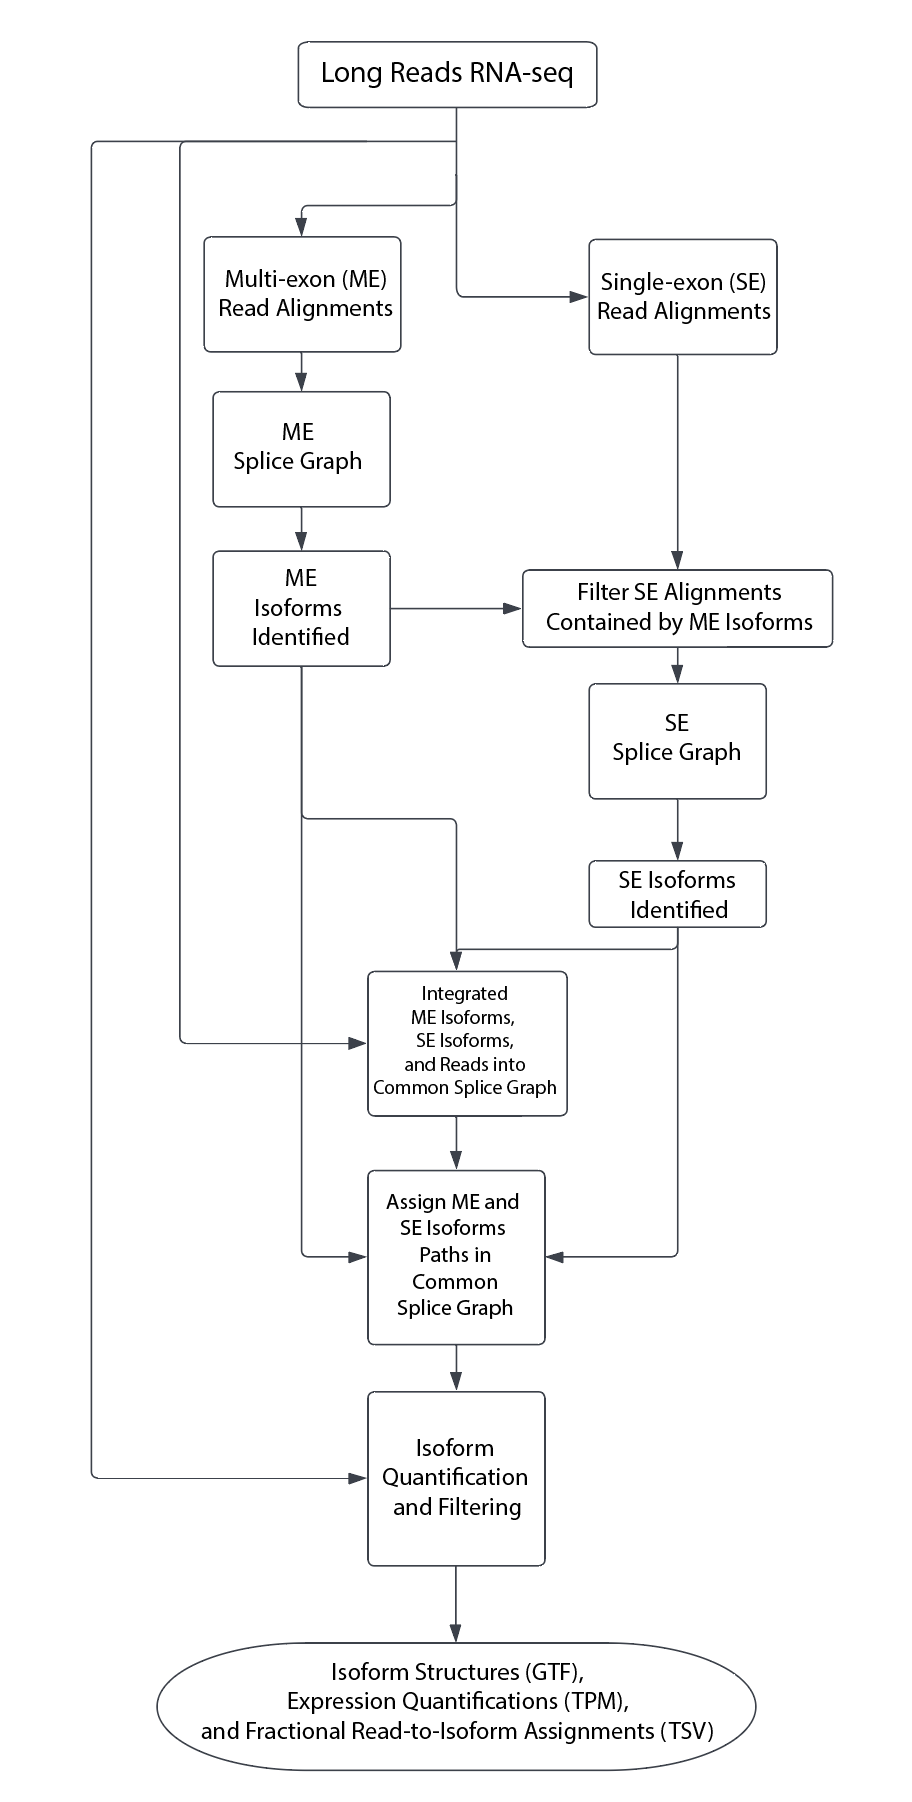
\includegraphics{figures/docx_export/SuppFig1.png}}
\end{center}

\captionof{figure}{LRAA high-level algorithm for isoform identification and quantification starting from aligned long RNA-seq reads. See \textbf{Methods} for detailed descriptions of stages.}\label{sfig:1}

\begin{center}
\pandocbounded{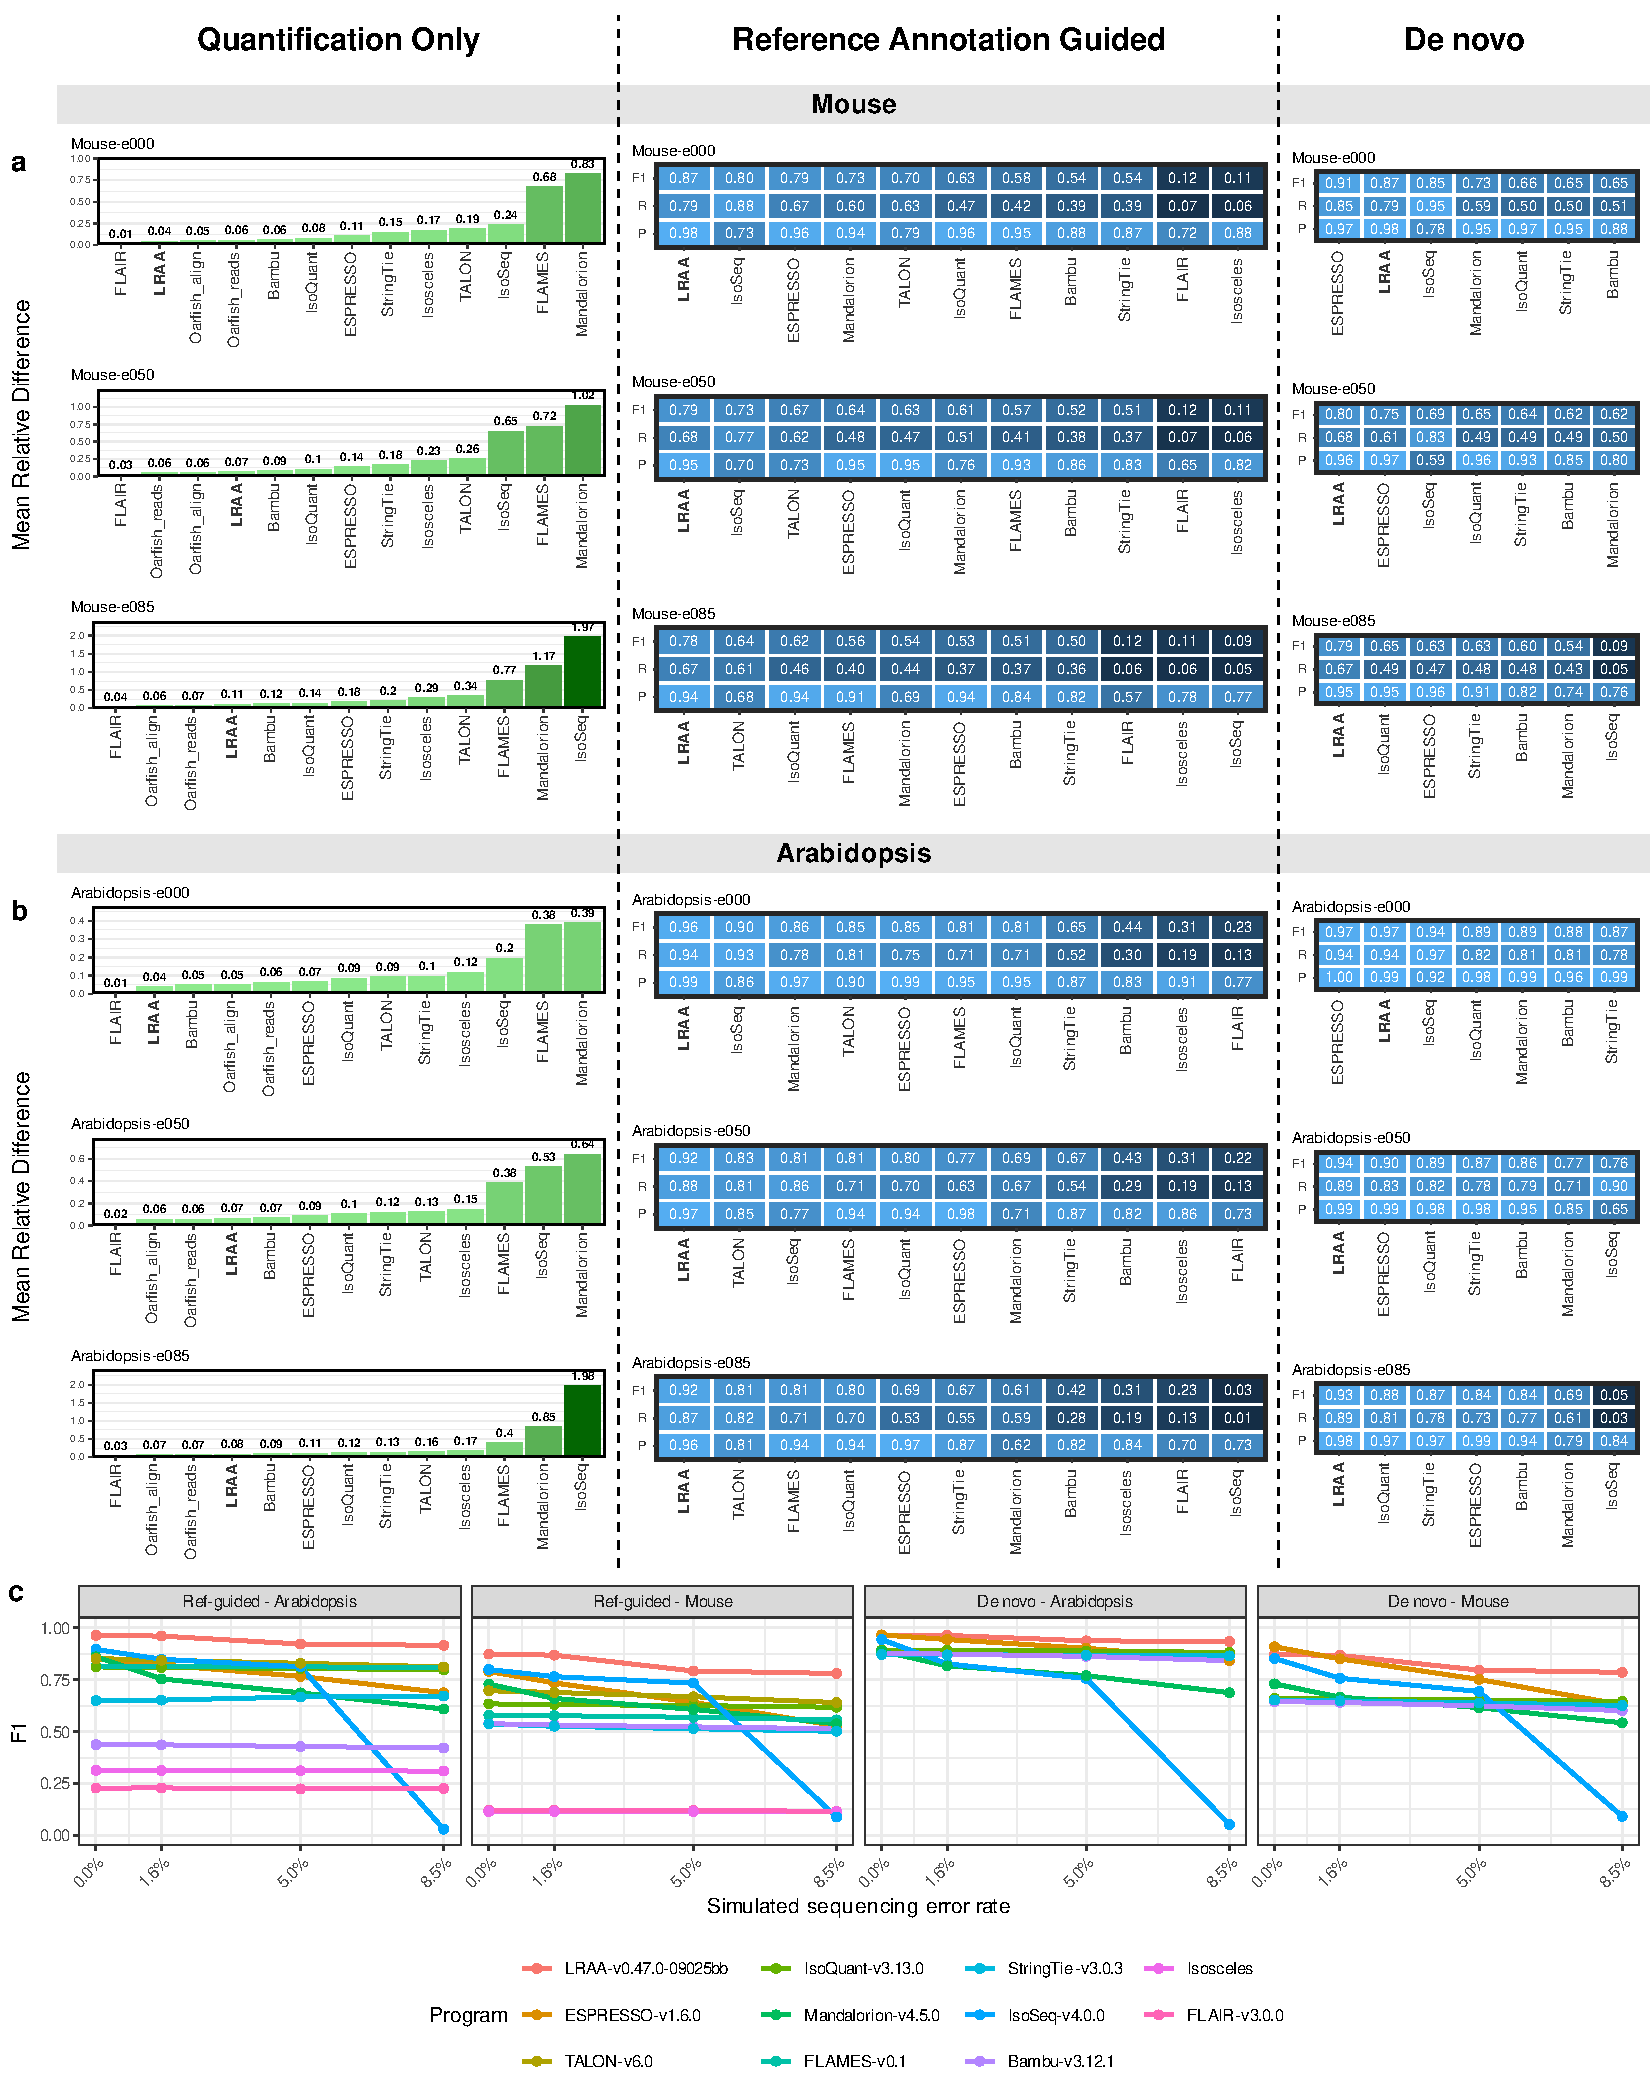
\includegraphics{figures/benchmark/SuppFig2_benchmarks_sim_error_rates.pdf}}
\end{center}

\captionof{figure}{Isoform quantification and identification accuracy based on (a) Mouse or (b) Arabidopsis simulated long RNA-seq at varied levels of sequencing error: e000: error-free, e050: 5\% error, and e085: 8.5\% error. (c) Isoform identification accuracy as a function of sequencing error according to model organism and execution mode.}\label{sfig:2}

\begin{center}
\pandocbounded{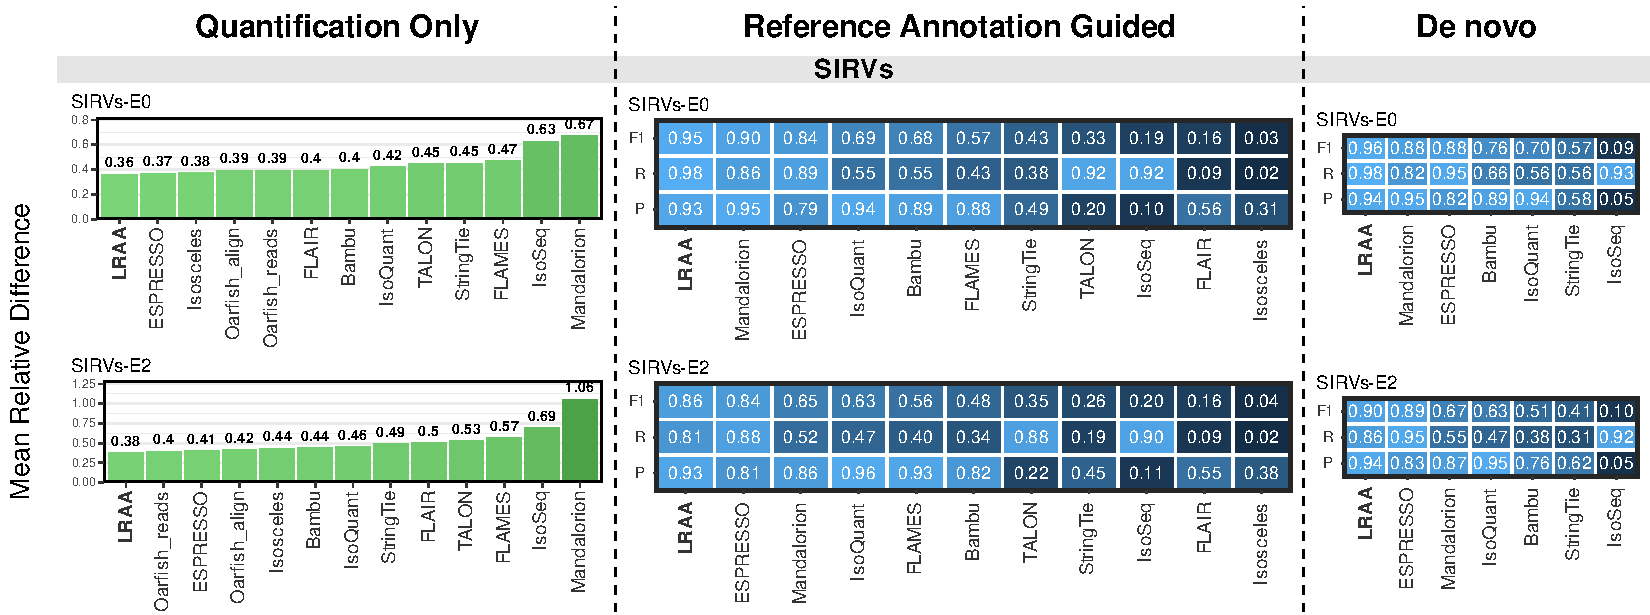
\includegraphics{figures/benchmark/SuppFig3_benchmarks_SIRVs_E0_E2.pdf}}
\end{center}

\captionof{figure}{Isoform ID and Quant accuracy for SIRV mixes E0 and E2.}\label{sfig:3}

\begin{center}
\makebox[\linewidth][l]{\sffamily\Large a}\par
\pandocbounded{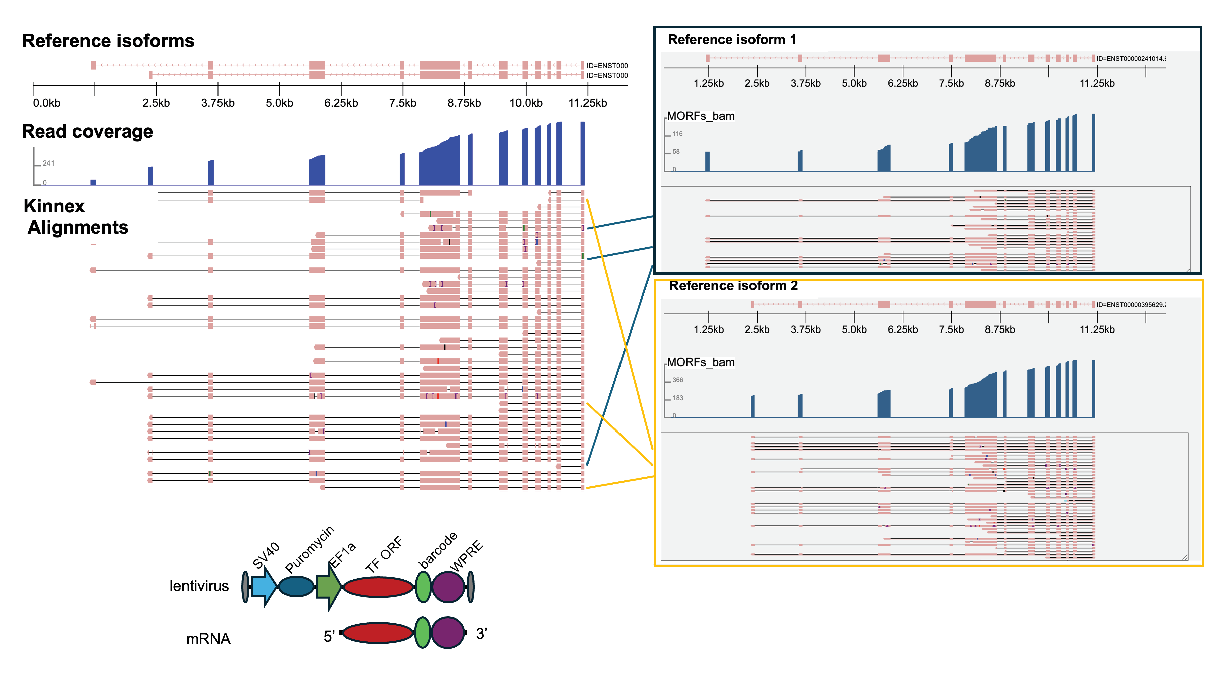
\includegraphics{figures/fixed/Supp_Fig_4-MORFsGenomeView.pdf}}

\medskip
\makebox[\linewidth][l]{\sffamily\Large b}\par
\pandocbounded{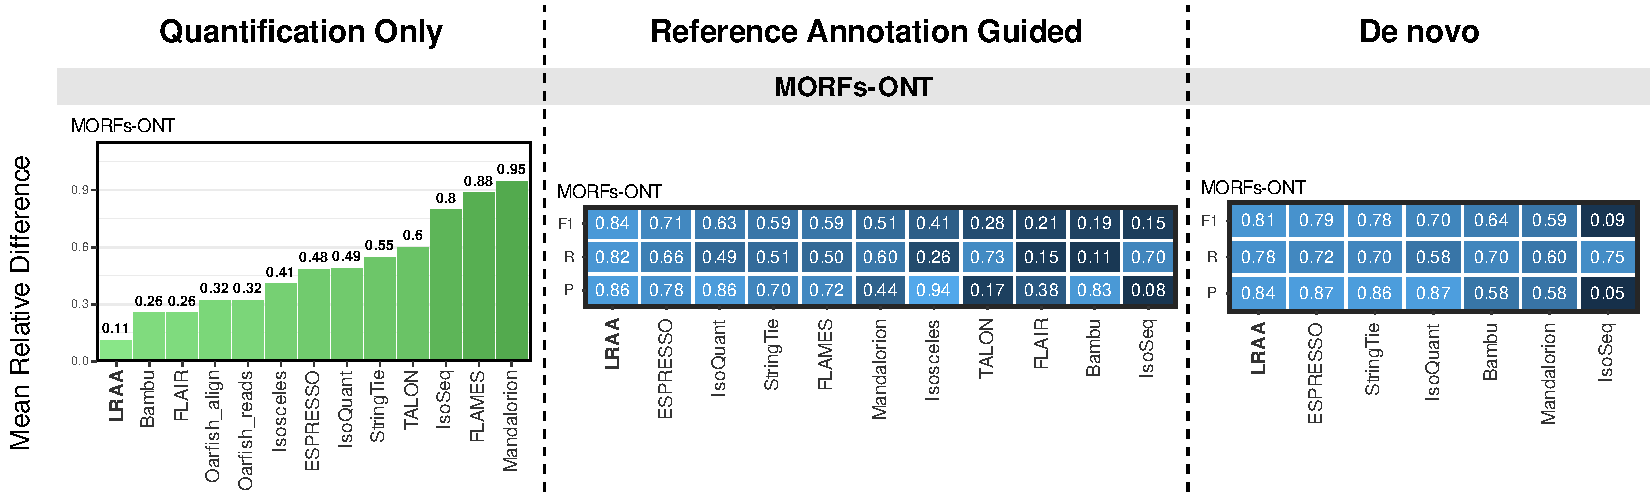
\includegraphics{figures/benchmark/SuppFig4b_benchmarks_MORFs_ONT.pdf}}
\end{center}

\captionof{figure}{Isoform ID and Quantitation using MORFs. (a) Barcoding strategy enabling unambiguous identification of isoform from which read was derived, regardless of read-to-isoform structure mapping uncertainty. MORF lentivirus construct and mRNA structures shown at bottom, adapted from \citep{joung2023}. (b) Quantification and isoform identification accuracy based on ONT long RNA-seq reads for MORFs.}\label{sfig:4}

\begin{center}
\pandocbounded{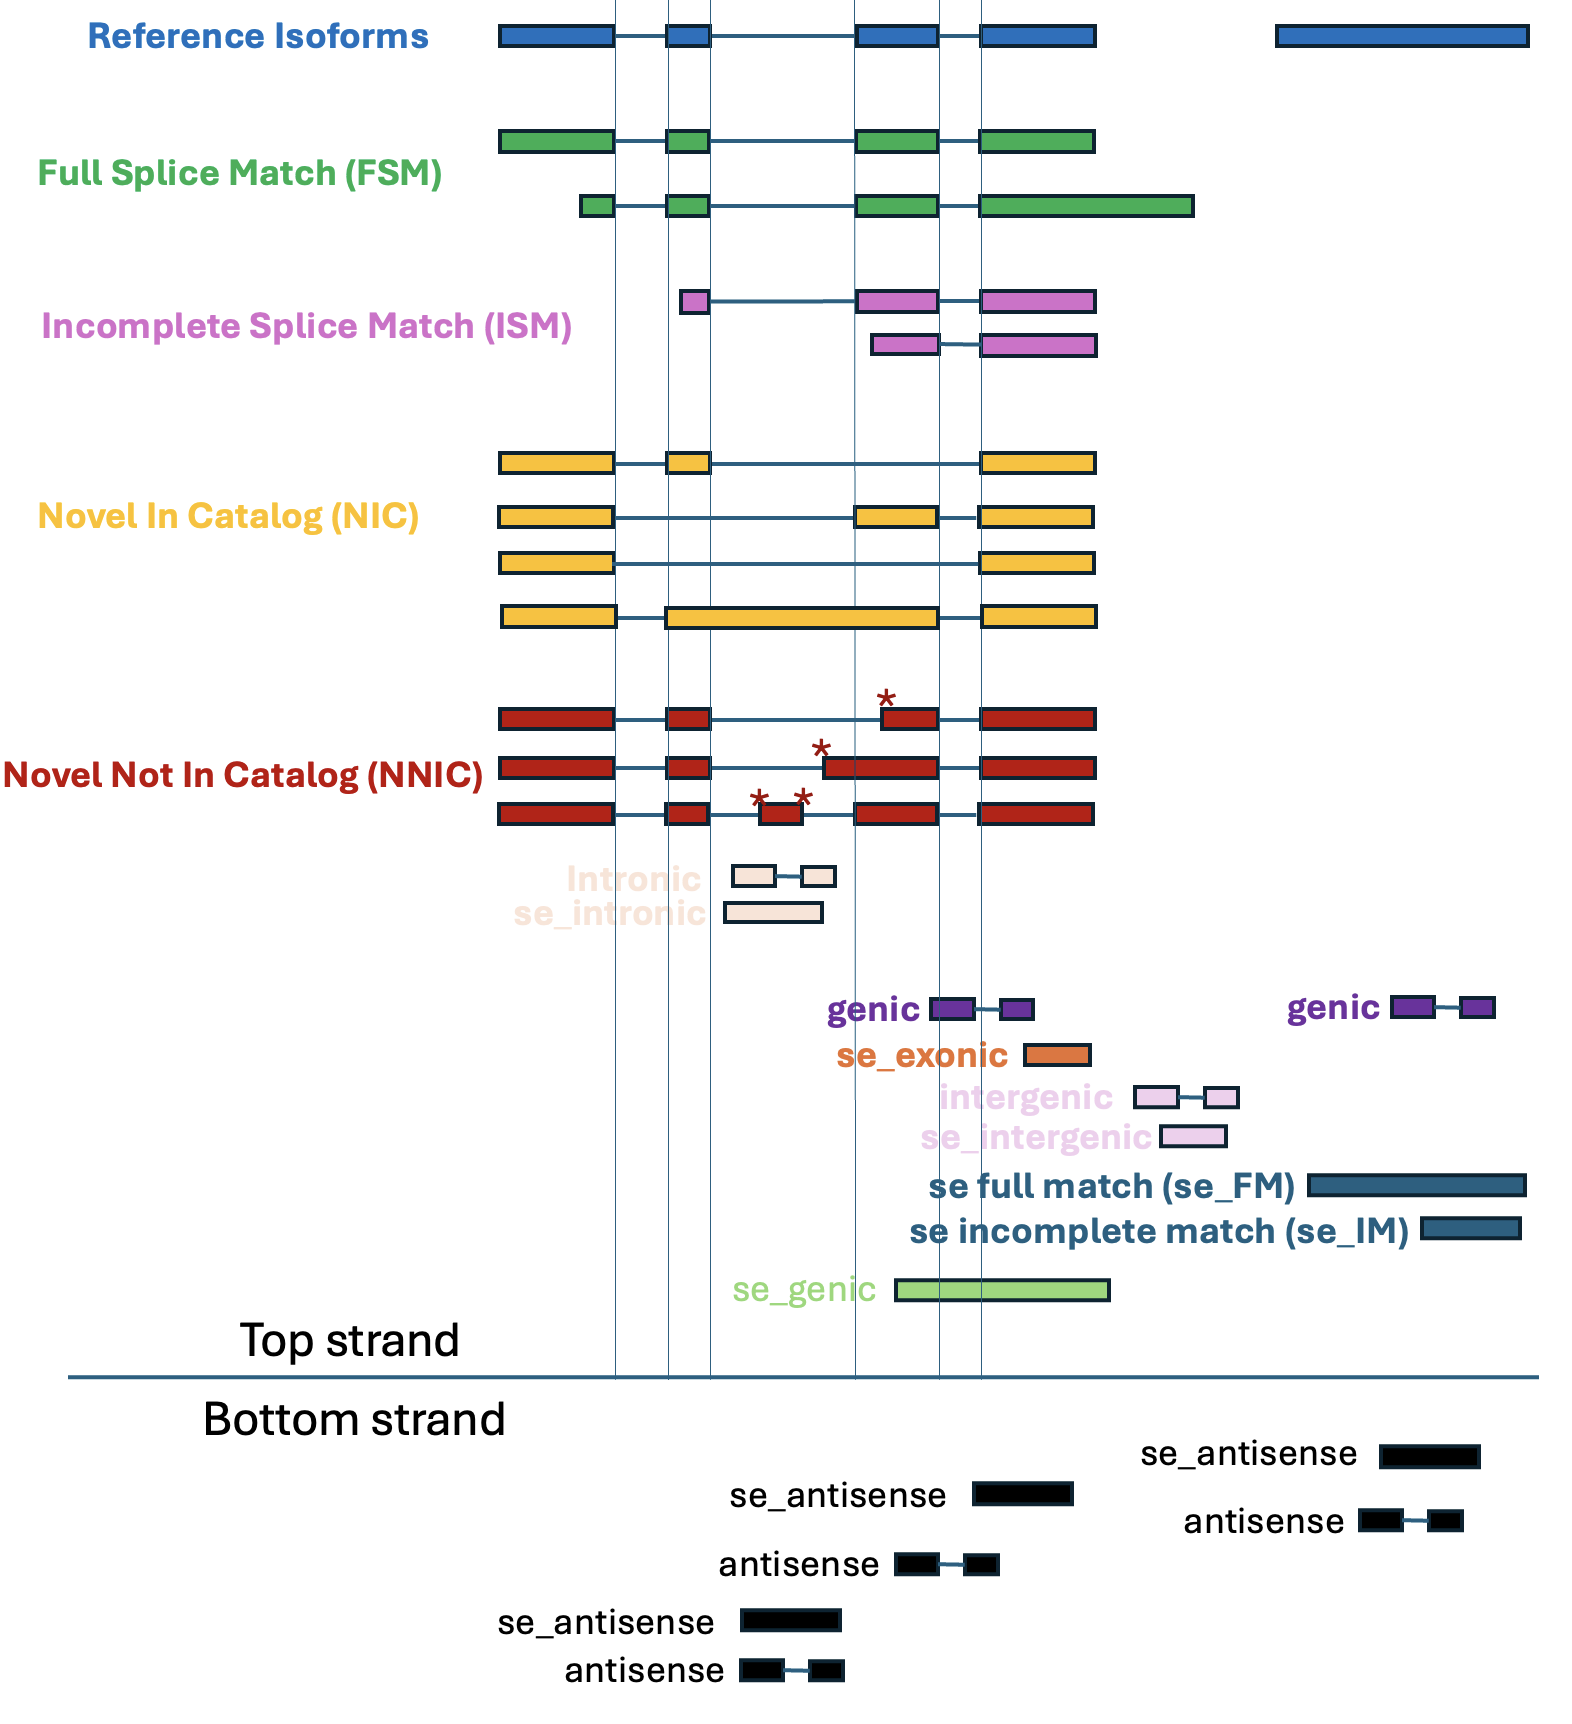
\includegraphics{figures/docx_export/SuppFig5.png}}
\end{center}

\captionof{figure}{LRAA's SQANTI-like classification scheme as applied to individual read alignments (BAM) or isoform structures (GTF) in comparison to a reference gene structure annotation (eg. GENCODE).}\label{sfig:5}

\begin{center}
\pandocbounded{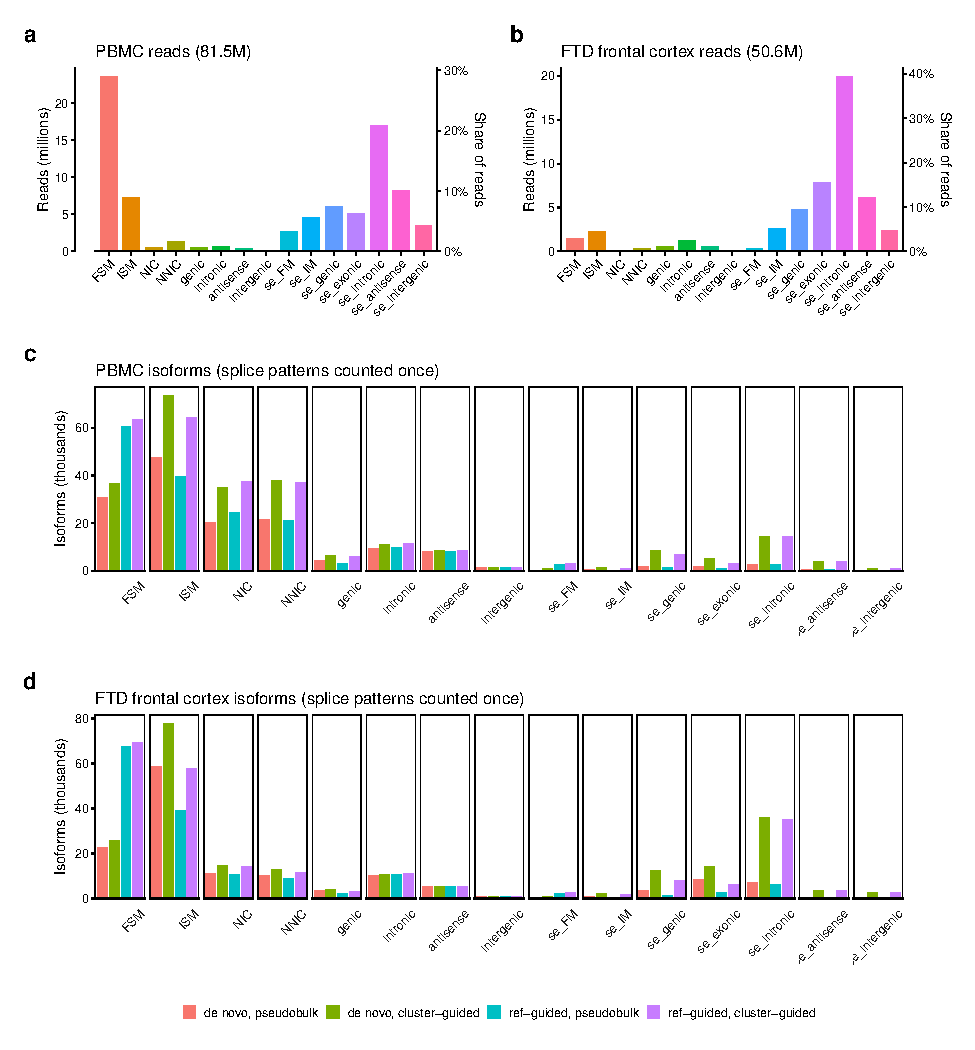
\includegraphics{figures/supp/SuppFig_categories.pdf}}
\end{center}

\captionof{figure}{SQANTI-like categories of the Kinnex reads and of the LRAA isoforms in the PBMC and FTD frontal cortex single-cell datasets. (a, b) Counts and percentages of Kinnex reads assigned to gene structures or genome regions according to LRAA SQANTI-like categories, for (a) PBMCs and (b) FTD frontal cortex. (c, d) Counts of LRAA-reconstructed isoforms from reference annotation-free (de novo) or reference annotation-guided workflows assigned to SQANTI-like categories, from the initial pseudobulk phase and the final cluster-guided phase, for (c) PBMCs and (d) FTD frontal cortex. Isoforms with identical splice patterns but different termini boundaries are counted non-redundantly as collapsed.}\label{sfig:cats}

\begin{center}
\pandocbounded{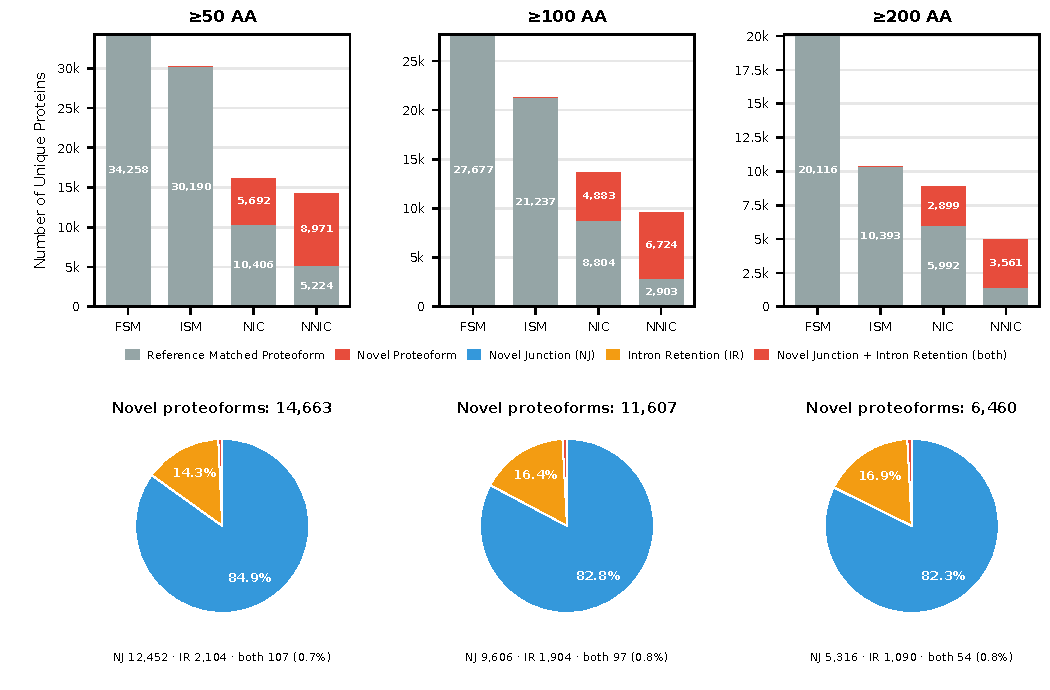
\includegraphics{figures/supp/SuppFig_proteoforms_PBMC.pdf}}
\end{center}

\captionof{figure}{Novel proteoform identification in human PBMCs. Top: Stacked bar charts showing unique protein counts by classification (FSM, ISM, NIC, NNIC) at ≥50 AA, ≥100 AA, and ≥200 AA thresholds. Proteins classified as Reference-Matched Proteoforms (gray) or Novel Proteoforms (red) based on splice junction novelty or intron retention within coding sequences. Bottom: Pie charts showing novel proteoform composition (NIC + NNIC) by splicing event type: Novel Junction only (blue), Intron Retention only (orange), or both (red); counts below each chart.}\label{sfig:6}

\begin{center}
\pandocbounded{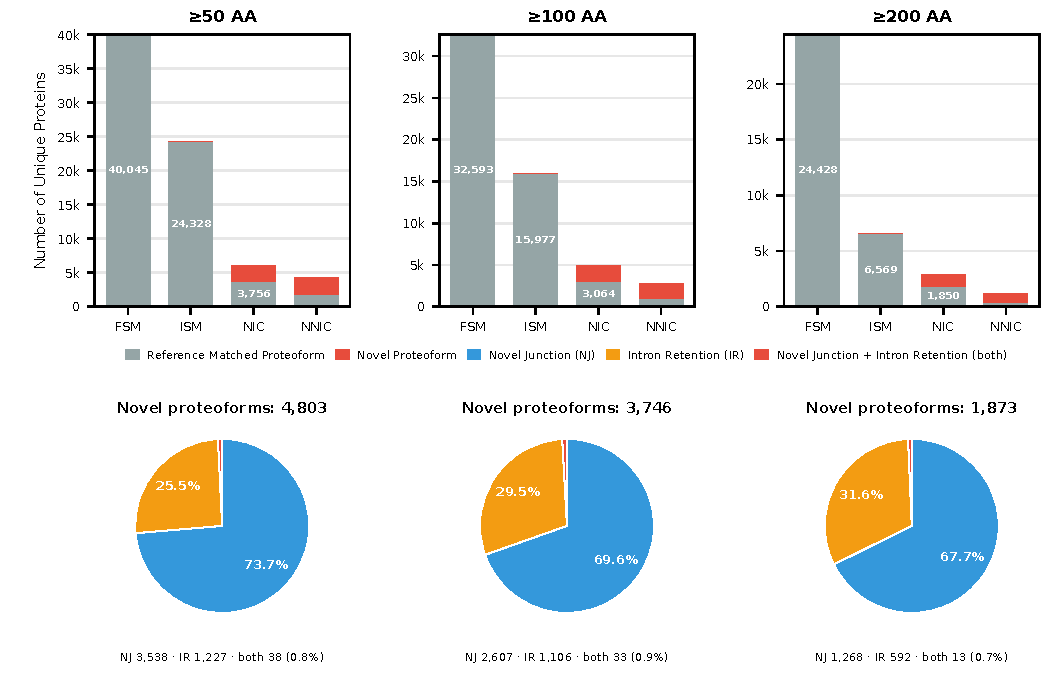
\includegraphics{figures/supp/SuppFig_proteoforms_FTD.pdf}}
\end{center}

\captionof{figure}{Novel proteoform identification in human FTD brain frontal cortex. Top: Stacked bar charts showing unique protein counts by classification (FSM, ISM, NIC, NNIC) at ≥50 AA, ≥100 AA, and ≥200 AA thresholds. Proteins classified as Reference-Matched Proteoforms (gray) or Novel Proteoforms (red) based on splice junction novelty or intron retention within coding sequences. Bottom: Pie charts showing novel proteoform composition (NIC + NNIC) by splicing event type: Novel Junction only (blue), Intron Retention only (orange), or both (red); counts below each chart.}\label{sfig:7}

\begin{center}
\pandocbounded{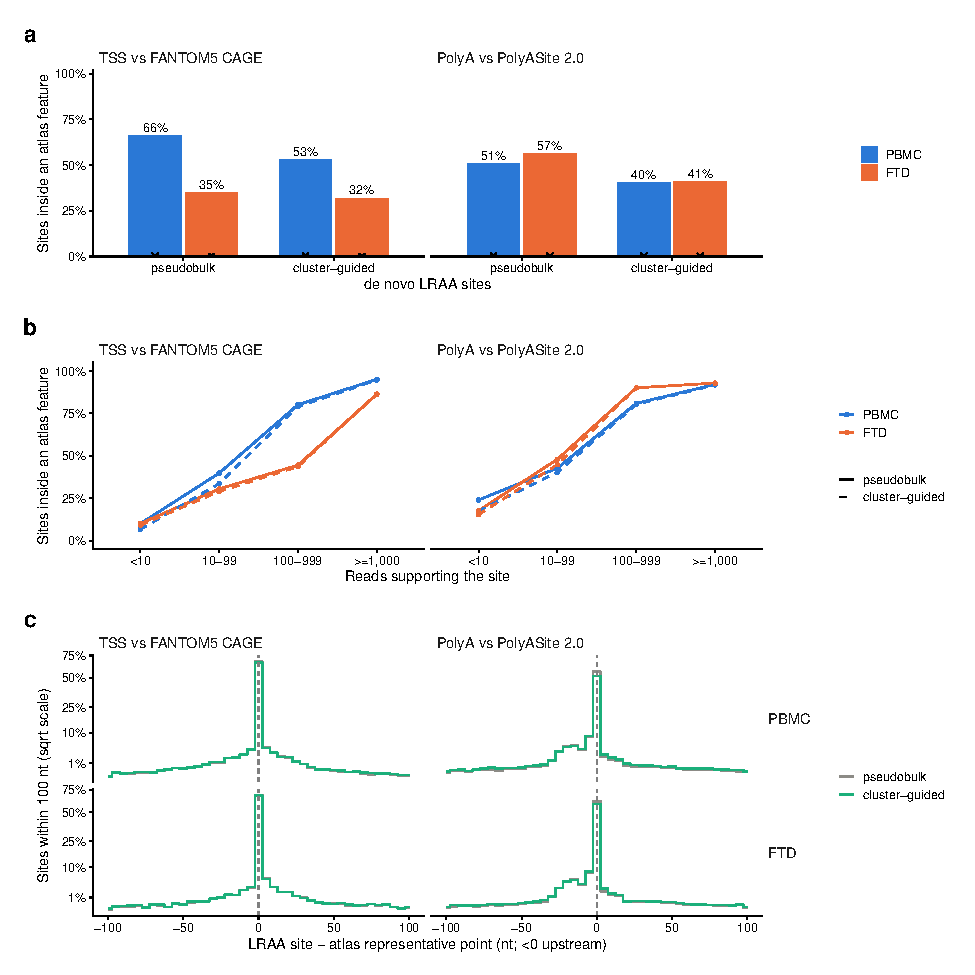
\includegraphics{figures/supp/SuppFig_site_atlas.pdf}}
\end{center}

\captionof{figure}{Agreement of LRAA's TSS and PolyA sites with FANTOM5 CAGE peaks and PolyASite~2.0 clusters in the PBMC and FTD frontal cortex datasets. Sites are those of the de novo runs (pseudobulk and cluster-guided), called from the reads alone. (a) Share of sites inside a same-strand atlas peak or cluster; crosses, the same sites placed at random within the LRAA transcript spans. (b) The same share by the number of reads supporting the site. (c) Signed offset of each site from the nearest atlas representative point (CAGE summit, PolyASite cleavage site), for sites within 100 nt, as a share of those sites per 5-nt bin (square-root scale).}\label{sfig:siteatlas}

\begin{center}
\pandocbounded{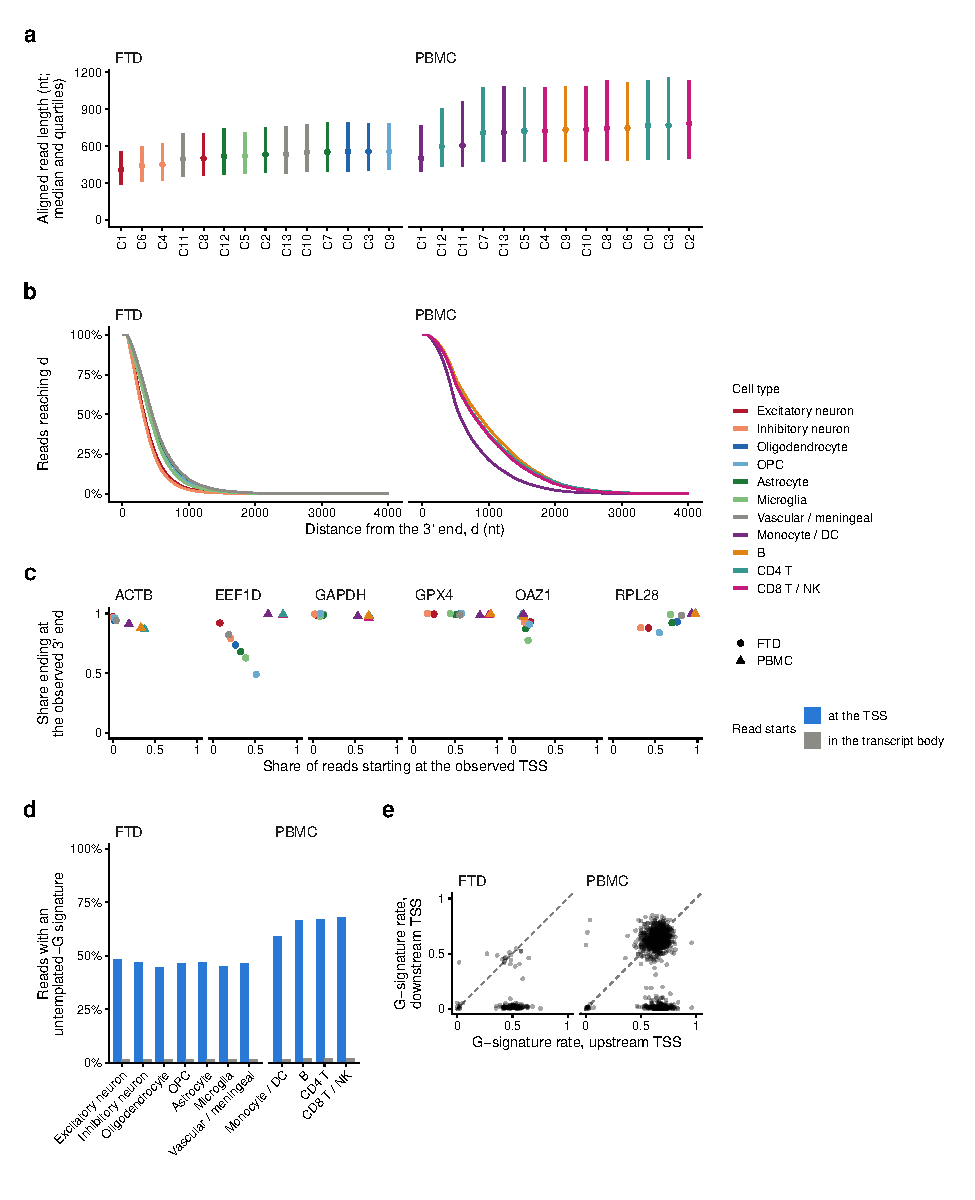
\includegraphics{figures/supp/SuppFig_TSS_5prime.pdf}}
\end{center}

\captionof{figure}{5\textquotesingle{} completeness of the reads and the untemplated-G signature, FTD frontal cortex nuclei and PBMCs. (a) Aligned read length by cluster (median and quartiles; a genome-wide sample of reads). (b) 5\textquotesingle{} completeness by cell type: the share of polyA-anchored reads reaching $d$ nt from the 3\textquotesingle{} end, averaged over genes with a single TSS. (c) Control genes: share of each cell type's reads starting at the observed TSS and ending at the observed 3\textquotesingle{} end (circles, FTD; triangles, PBMC). (d) Share of reads carrying an untemplated G at the 5\textquotesingle{} end, for reads starting at the TSS and inside the transcript body of genes with a single TSS. (e) The same signature at the upstream and downstream sites of each high-confidence TSS switch called before LRAA used the cap signature (LRAA version 0.45.0; site pairs with at least 20 informative reads at each site), counting a read as capped by LRAA's definition (\textbf{Methods}). (d, e) Reads whose genomic base upstream of the 5\textquotesingle{} end is not G. See \textbf{Methods}.}\label{sfig:tss5prime}

\clearpage
\section*{Supplementary Tables}

\noindent\textbf{Supplementary Table 1.} High-confidence differential isoform usage events between cell clusters in the PBMC and FTD frontal cortex datasets (DEXSeq on pseudo-replicates; \textbf{Methods}), one sheet per dataset and level: splice patterns, and TSS and PolyA sites tested on read ends, with each site switch's splicing class (tandem or coupled with alternative splicing) and the LRAA isoforms carrying its two sites. The FTD TSS switches are listed with a caveat: some may be 5\textquotesingle{} truncation products (\textbf{Results}). Each row is a gene and pair of clusters, with the gained and lost features, their usage, read counts and unique full-length reads in each cluster, the pairwise adjusted P values, and the switch class. A README sheet defines the columns, and a Summary sheet gives the number of genes tested, significant, with events and with high-confidence events at each level.


\end{document}
